\chapter{Spread Spectrum, CDMA and Satellite Navigation}
\label{ch:spreadspectrum}

\begin{chapterintro}
Most of this book is about using bandwidth sparingly. This chapter is about the opposite
choice: deliberately smearing a signal over a band hundreds or thousands of times wider than its
data need---and getting something precious in return. The idea began as a military secret
(signals an enemy cannot jam, cannot find and cannot read) and grew into the second-generation
cellular standard IS-95, all three big third-generation standards, the first Wi-Fi and Bluetooth.
Most remarkably of all, it is how satellite navigation works. Every GPS, Galileo, GLONASS and
BeiDou receiver digs a signal out from \emph{under} the thermal noise, times its arrival to a few
nanoseconds, and from four or more such measurements works out where it is and what time it is.

We start with why anyone would spread, and with the clever binary sequences that make it possible
(m-sequences, Gold, Kasami and Walsh codes). Then direct-sequence and frequency-hopping spread
spectrum and how they shrug off jammers; code-division multiple access, with its near--far
problem, power control, soft handoff, capacity formula, Rake receiver and multiuser detectors;
and two cousins, the chirps of LoRa and the picosecond pulses of ultra-wideband ranging. The
second half is a full tour of satellite navigation: the story of GPS, the pseudorange equation and
its solution, the signals, the receiver from antenna to position fix, the error budget and the
corrections that shrink it to centimetres, Einstein's contribution, and the fragility of a
civilisation that takes its time and position from signals weaker than $10^{-16}$\,W.
Figure~\ref{fig:ch18_by_numbers} previews the numbers we will meet along the way.
\end{chapterintro}

\begin{figure}[!h]\centering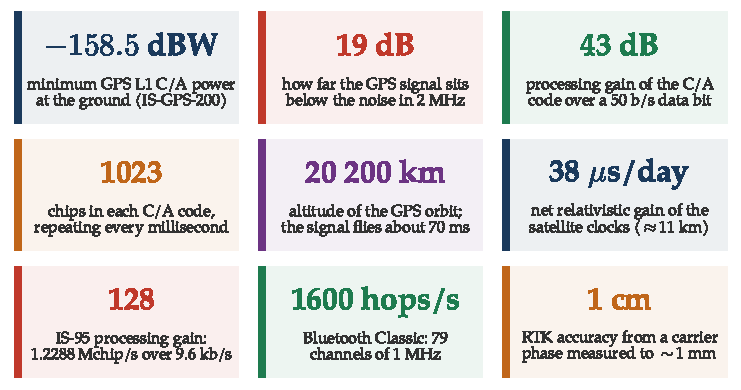
\includegraphics[width=0.9\linewidth]{figs/ch18_by_numbers}
\caption{Spread spectrum and satellite navigation by the numbers. Every one of
these values is derived or explained somewhere in this chapter.}\label{fig:ch18_by_numbers}\end{figure}

%======================================================================
\section{Why spread?}
\label{sec:ch18:why}
%======================================================================

Here is a puzzle. A 9.6\,kb/s voice channel needs roughly 10\,kHz of bandwidth, yet the IS-95
cellular standard sent it in 1.25\,MHz. A GPS satellite sends its 50\,b/s navigation message in
about 2\,MHz, and its military signal in 20\,MHz. Everything in Chapters~\ref{ch:modulation}
and~\ref{ch:infotheory} pushes us towards more bits per hertz, and here are systems that
cheerfully run at a few \emph{thousandths} of a bit per hertz. Are their designers mad?

They are not, and the reason is one of the most beautiful trades in engineering. Think of
whispering a secret across a crowded, noisy room. Instead of saying it once, loudly, you spread
it over a hundred quiet voices scattered around the room, each saying a tiny piece in a pattern
that only your friend knows. To everyone else the room just sounds a little noisier. Your friend,
who knows the pattern, listens to exactly those voices in exactly that order and hears your
secret clearly. Someone shouting in one corner hardly bothers her, because she was only listening
to that corner for a moment. That, in one paragraph, is spread spectrum.

\subsection{What ``spread spectrum'' means}

A signal is a \term{spread-spectrum} signal when two conditions hold:
\begin{enumerate}
\item its bandwidth $W$ is much larger than the minimum needed for the information rate
$R$, typically by a factor of 10 to $10^4$; and
\item the spreading is done by a \emph{code} (a pseudo-random sequence known to the
intended receiver) that is independent of the data, and the receiver undoes it by
correlating with a synchronised copy of the same code.
\end{enumerate}
The second condition is essential. Wideband FM also uses far more bandwidth than the audio
it carries (Chapter~\ref{ch:analog}), but the spreading is done by the message itself and
anyone can demodulate it. In spread spectrum the spreading is done by the code, and without
the code the signal looks like noise.

Figure~\ref{fig:ch18_spread_concept} shows the simplest version in the time domain. Each data
bit is chopped into many short \emph{chips} by a fast pseudo-random $\pm1$ code. The product
wiggles $G_p$ times faster than the data, so its spectrum is $G_p$ times wider. Multiply by the
same code again and every chip is squared back to $+1$: the data reappear untouched.

\mdcfig{ch18_spread_concept}{Direct-sequence spreading in the time domain. Each data bit (top) is
multiplied by 15 chips of a pseudo-noise code (middle). The transmitted waveform (bottom) changes
sign 15 times faster than the data, so it occupies 15 times the bandwidth. A receiver that
multiplies by the same code, chip for chip, gets the top trace back, because $c^2(t)=1$.}

The ratio
\begin{equation}
G_p=\frac{W}{R}\approx\frac{T_b}{T_c}
\label{eq:ch18:gp}
\end{equation}
is the \term{processing gain}, where $T_b$ is the bit (or symbol) duration and $T_c$ the
\term{chip} duration, the shortest element of the spreading code. It is usually quoted in
decibels: IS-95 has $G_p=1.2288\times10^6/9600=128$, or 21\,dB; GPS C/A has
$1.023\times10^6/50=20\,460$, or 43\,dB.

There are four ways to spread:
\begin{description}[style=nextline,leftmargin=1.2em,font=\sffamily\bfseries\small\color{navy}]
\item[Direct sequence (DSSS).] Multiply the data by a fast pseudo-random $\pm1$ chip
sequence. The spectrum widens to the chip rate. Used by GPS, IS-95, WCDMA and 802.11b.
\item[Frequency hopping (FHSS).] Change the carrier frequency according to a pseudo-random
pattern. At any instant the signal is narrowband, but over time it covers a wide band. Used
by Bluetooth, military VHF radios and Link-16.
\item[Time hopping.] Send short pulses at pseudo-random times within each frame. The basis of
impulse-radio ultra-wideband.
\item[Chirp spread spectrum.] Sweep the carrier linearly across the band. Used in radar pulse
compression and in LoRa.
\end{description}
Hybrids are common: Link-16 combines direct sequence with fast frequency hopping, and
Bluetooth's slow hopping carries a narrowband GFSK signal in each hop.

\subsection{Shannon's view: bandwidth is not wasted}

Why is throwing bandwidth at a signal not as wasteful as it looks? Shannon answers it. The
capacity of an AWGN channel of bandwidth $W$ with received power $S$ and noise
density $N_0$ is (Chapter~\ref{ch:infotheory})
\begin{equation}
C=W\log_2\!\left(1+\frac{S}{N_0W}\right)\;\xrightarrow{\;W\to\infty\;}\;\frac{S}{N_0\ln2}.
\end{equation}
In words: at low SNR, capacity depends on power, not bandwidth, so spreading a signal over more
bandwidth costs almost nothing in achievable rate. A spread-spectrum system is simply a system that
has chosen to operate in the power-limited regime, far to the left of the capacity curve,
and spends the extra bandwidth on something other than bits. It spends it on resistance to
interference, on hiding, on resolving multipath, on sharing the band and on measuring time.
Spreading gives no advantage against white Gaussian noise, though
(Section~\ref{sec:ch18:awgn}): a DSSS link has exactly the bit error rate of the
unspread link at the same $\ebno$.

\mdcfig[0.55]{ch18_cocktail}{Why correlation works (simulated, random $\pm1$ codes). The output
for the code you are listening for grows like $N$; the output for any other code is a random walk
that grows only like $\sqrt N$. Their ratio in power is $N=G_p$.}

\subsection{Five reasons to spread}

\begin{enumerate}
\item \textbf{Anti-jamming.} A jammer with finite power must either concentrate it in a
narrow band, where the receiver's despreading dilutes it by $G_p$, or spread it over the
whole band, where its density is low. Either way the receiver gains roughly a factor $G_p$
(Section~\ref{sec:ch18:jamming}).
\item \textbf{Low probability of intercept and detection (LPI/LPD).} The power spectral
density of a spread signal can be far below the thermal noise density. An adversary who
does not know the code sees a slight rise in the noise floor, if anything.
\item \textbf{Multipath resolution.} Correlation with the code produces a peak about one chip
wide. Echoes delayed by more than a chip produce separate peaks that can be separated and
combined (the Rake receiver, Section~\ref{sec:ch18:rake}). A 3.84\,Mchip/s WCDMA signal
resolves paths 78\,m apart in path length.
\item \textbf{Multiple access.} Users with different codes can share the same band at the same
time; each receiver's correlator passes its own signal and suppresses the others by
roughly $G_p$. This is code-division multiple access, CDMA (Section~\ref{sec:ch18:cdma}).
\item \textbf{Ranging and timing.} The arrival time of a wideband signal can be measured to a
small fraction of a chip. With a 1\,$\mu$s chip, a correlator measures delay to a few
nanoseconds, which is what makes GNSS positioning possible (Section~\ref{sec:ch18:gnss}).
Chapter~\ref{ch:sync} showed that timing accuracy scales with bandwidth (the Cram\'er--Rao
bound); spreading is the way to buy bandwidth without buying data rate.
\end{enumerate}

\begin{analogy}[An ear trained to one voice]
At a noisy cocktail party you can follow your friend's voice across the room while thirty other
conversations wash over you. Your brain is correlating: it knows the rhythm, pitch and accent it
is waiting for, so every syllable of your friend's speech adds up, while the others, uncorrelated
with what you expect, add up only as a blur. A spread-spectrum correlator does exactly this with
chips. Figure~\ref{fig:ch18_cocktail} measures it: after $N$ chips the wanted code has piled up an
output of $N$, while any other code has managed only about $\sqrt N$. Where the analogy breaks:
your brain cannot pull a voice out from 20\,dB \emph{below} the babble. A correlator with
enough chips can.
\end{analogy}

\mdcfig[0.98]{ch18_timeline}{Eighty years of spread spectrum and satellite navigation. Military
secrecy (grey and navy) gave way to cellular CDMA and unlicensed radio (red and orange) and to
satellite navigation (green), which is now the largest civil use of spread spectrum by far.}

\begin{keyidea}[Processing gain is a trade]
Spreading does not create energy, and it does not help against white noise. What it does
is make the wanted signal \emph{coherent} with the receiver's code while everything
else---narrowband jammers, other users, echoes at other delays---stays incoherent. The
correlator adds $G_p$ chips of the wanted signal in amplitude (a gain of $G_p^2$ in power)
but adds the interference only in power (a gain of $G_p$). The ratio, $G_p$, is the
processing gain. Every application in this chapter is a way of spending it.
\end{keyidea}

\mdcphoto[0.45]{ch18_lamarr_patent}{The first page of US Patent 2,292,387, ``Secret Communication
System'', by Hedy Kiesler Markey (Hedy Lamarr) and George Antheil, filed June 1941: a radio-guided
torpedo whose carrier hops among 88 frequencies under the control of synchronised paper rolls.}

\begin{history}[Hedy Lamarr, George Antheil and the piano roll]
In June 1941 the film actress Hedy Lamarr and the composer George Antheil filed a patent for a
``Secret Communication System'' (Figure~\ref{fig:ch18_lamarr_patent}). It was granted as US
Patent 2,292,387 on 11~August 1942. The idea was to guide a torpedo by radio while hopping the
carrier among 88 frequencies---the number of keys on a piano---in a pattern stored on two
synchronised paper rolls like those of a player piano, one in the ship and one in the torpedo. An
enemy could not jam a signal whose frequency he did not know. Lamarr had learned something of
weapons engineering from her first husband, an Austrian arms manufacturer; Antheil had
synchronised sixteen player pianos for his \emph{Ballet M\'ecanique}. The US Navy did not adopt
the invention, and the patent expired unused.

The patent's real significance is sometimes overstated. It did not invent frequency hopping
(earlier proposals existed), it was not the origin of the direct-sequence techniques behind
GPS and CDMA, and there is no line of engineering descent from it to Wi-Fi or Bluetooth. What
it did contain was a clear statement of the essential principle---a shared secret pattern,
synchronised at both ends, that makes the signal unpredictable to anyone else---two decades
before electronics could implement it cheaply. Lamarr's contribution was recognised late,
with an Electronic Frontier Foundation Pioneer Award in 1997, and she is now an emblem of the
inventors whom history overlooked.
\end{history}

\begin{history}[From SIGSALY to the Rake: the secret years]
The first operational system that hid speech under a noise-like key was SIGSALY, built by
Bell Telephone Laboratories in 1942--43 for telephone conversations between Churchill and
Roosevelt. It digitised speech with a vocoder into slowly varying levels and added to them,
modulo six, a key taken from phonograph records of recorded thermal noise, of which only two
copies existed and which were destroyed after use. It was a one-time pad, not spread
spectrum, but it established the idea of a shared noise-like reference.

After the war, spread spectrum proper was developed in secret. The MIT Lincoln Laboratory
NOMAC system (``noise modulation and correlation'') of the early 1950s spread data with a
noise-like waveform and recovered it by correlation, and its successor, the F9C system,
operated on long-haul HF links where multipath smeared the signal. Robert Price and Paul
Green's solution to that smearing, published in 1958, was the Rake receiver. Through the Cold
War spread spectrum carried military satellite links, missile guidance and command links
that had to survive jamming, and the details stayed classified until the 1970s. Robert
Scholtz's 1982 history of the field (see Further Reading) pieced the story together from the
participants. Figure~\ref{fig:ch18_timeline} puts these milestones alongside the civil story that
followed.
\end{history}

%======================================================================
\begin{figure}[htbp]\centering
\begin{tikzpicture}[cell/.style={draw=navy,fill=navy!6,thick,minimum size=0.75cm,font=\sffamily\small},
  xo/.style={draw=accent,circle,thick,minimum size=0.5cm,inner sep=0pt,font=\small},
  arr/.style={-{Stealth[length=2mm]},thick,navy}]
\node[cell] (c1) at (0,0) {$a_{k+2}$};
\node[cell] (c2) at (1.2,0) {$a_{k+1}$};
\node[cell] (c3) at (2.4,0) {$a_{k}$};
\draw[arr] (c1) -- (c2); \draw[arr] (c2) -- (c3);
\draw[arr] (c3.east) -- ++(1.3,0) node[right,font=\sffamily\scriptsize,align=left] {output chips\\0\,0\,1\,0\,1\,1\,1\,\dots};
\node[xo] (x) at (1.8,1.2) {$\oplus$};
\draw[navy,thick] (c2.north) |- (x.west);
\draw[navy,thick] ([xshift=0.4cm]c3.east) |- (x.east);
\draw[arr] (x.north) -- ++(0,0.35) -| ([xshift=-0.55cm]c1.west) -- (c1.west);
\node[font=\sffamily\scriptsize,text=navy!70,align=center] at (1.2,-0.8) {clock: one shift per chip};
\node[font=\sffamily\scriptsize,text=accent] at (3.7,1.65) {$a_{k+3}=a_{k+1}\oplus a_k$};
\node[font=\sffamily\scriptsize,text=green!40!black,align=left,anchor=west] at (6.6,0.3)
 {states visited:\\001, 010, 101, 011,\\111, 110, 100, then repeat\\(all 7 non-zero states)};
\end{tikzpicture}
\caption{A three-stage linear feedback shift register for $p(x)=x^3+x+1$. Two flip-flop outputs are
XORed and fed back; the register cycles through all seven non-zero states before repeating, so the
output is an m-sequence of period 7. The GPS C/A generator (Figure~\ref{fig:ch18_cagen}) is the same
idea with two ten-stage registers.}
\label{fig:ch18_lfsr}
\end{figure}

\section{Pseudo-noise sequences}
\label{sec:ch18:pn}
%======================================================================

How do you make a sequence that looks perfectly random to everyone else, yet which your friend
can reproduce exactly, chip for chip, billions of chips later? A spreading code must be balanced,
with no structure an interferer or an eavesdropper can exploit, and with a sharp autocorrelation
so the receiver can find it and measure its delay---yet it must be exactly reproducible by the
intended receiver. Such deterministic sequences with random-like properties are called
\term{pseudo-noise} (PN) sequences. Chapter~\ref{ch:sync} used them as synchronisation
preambles; here they carry the whole signal. Remarkably, the best of them come from a few
flip-flops and an exclusive-OR gate.

\subsection{Linear feedback shift registers}

The workhorse generator is the \term{linear feedback shift register} (LFSR): $m$ binary
storage cells, shifted once per chip, with the new input formed as the exclusive-OR of
selected cells (Figure~\ref{fig:ch18_lfsr}). The output obeys the linear recurrence
\begin{equation}
a_{k+m}=c_{m-1}a_{k+m-1}\oplus\cdots\oplus c_1a_{k+1}\oplus c_0a_k,
\label{eq:ch18:lfsr}
\end{equation}
with $c_0=1$. The recurrence is described by its \term{characteristic polynomial}
$p(x)=x^m+c_{m-1}x^{m-1}+\cdots+c_1x+1$ over GF(2). Because the register has $2^m$ states
and the all-zero state maps to itself, the output is periodic with period at most $2^m-1$.
It reaches that maximum exactly when $p(x)$ is a \term{primitive polynomial}, one whose
roots generate the multiplicative group of the finite field GF($2^m$)
(Chapter~\ref{ch:classiccodes} develops finite fields). The output is then a
\term{maximal-length sequence}, or \term{m-sequence}, of period $N=2^m-1$: the register visits
every non-zero state exactly once before repeating, like an odometer that has been rewired to
count in a scrambled order. There are $\phi(2^m-1)/m$ primitive polynomials of degree $m$, where
$\phi$ is Euler's totient: 6 for $m=5$, 60 for $m=10$, and 1800 for $m=15$.

There are two equivalent hardware forms. The \emph{Fibonacci} (external-XOR) form computes
one parity of several cells and feeds it back to the input, as in~\eqref{eq:ch18:lfsr}. The
\emph{Galois} (internal-XOR) form XORs the output bit into several cells as it shifts; it
produces the same sequence at a different phase and is faster in hardware because each
stage has at most one XOR gate in its path. Software implementations use word-wide Galois
LFSRs, or simply store the code in a table: a GPS receiver's 1023-chip codes occupy 128
bytes each.

\mdcfig{ch18_mseq}{The m-sequence's near-perfect correlation. (a) The periodic autocorrelation of a
length-31 m-sequence: a spike of 31 every period and a flat floor of exactly $-1$ in between. (b)
Its spectrum is a comb of lines $R_c/N$ apart under the $\sinc^2$ envelope of a random chip stream,
as in~\eqref{eq:ch18:pnpsd} (drawn for $N=15$ so the lines can be seen).}

\begin{worked}[An m-sequence by hand]
Take $p(x)=x^3+x+1$, which is primitive, so $a_{k+3}=a_{k+1}\oplus a_k$. Starting from
$a_0a_1a_2=001$:
\[
a=0\,0\,1\,0\,1\,1\,1\;|\;0\,0\,1\,0\,1\,1\,1\;|\;\dots
\]
The period is $7=2^3-1$, and every non-zero 3-bit pattern appears exactly once in a sliding
window: $001,010,101,011,111,110,100$. There are four ones and three zeros. Mapping
$0\to+1$, $1\to-1$ gives $c=(+1,+1,-1,+1,-1,-1,-1)$, and the periodic autocorrelation
$R(k)=\sum_nc_nc_{n+k}$ is
\[
R(0)=7,\qquad R(1)=R(2)=\dots=R(6)=-1.
\]
Try $k=1$: the products $c_nc_{n+1}$ are $+1,-1,-1,-1,+1,+1,-1$, which sum to $-1$. The
reason is the shift-and-add property below.
\end{worked}

\subsection{Properties of m-sequences}

M-sequences have three ``randomness'' properties, first catalogued by Solomon Golomb in the
1950s. They are the same properties you would expect from a fair coin tossed many times:
\begin{enumerate}
\item \textbf{Balance.} One period contains $2^{m-1}$ ones and $2^{m-1}-1$ zeros.
\item \textbf{Runs.} Half the runs (maximal strings of identical symbols) have length 1,
a quarter length 2, an eighth length 3, and so on, as in a fair coin-toss sequence. The
longest run is $m$ ones.
\item \textbf{Shift-and-add.} The modulo-2 sum of an m-sequence and any cyclic shift of it is
another cyclic shift of the same sequence. This follows from linearity: both sequences
satisfy~\eqref{eq:ch18:lfsr}, so their sum does too, and it is not the zero sequence.
\end{enumerate}
The third property gives the autocorrelation at once. With $c_n=(-1)^{a_n}$, the product
$c_nc_{n+k}=(-1)^{a_n\oplus a_{n+k}}$ and $a_n\oplus a_{n+k}$ is itself an m-sequence for
$k\ne0$, so it has one more $-1$ than $+1$:
\begin{equation}
R(k)=\sum_{n=0}^{N-1}c_nc_{n+k}=\begin{cases}N,&k\equiv0\pmod N,\\-1,&\text{otherwise.}\end{cases}
\label{eq:ch18:mseqacf}
\end{equation}
This two-valued periodic autocorrelation (Figure~\ref{fig:ch18_mseq}a) is as close to an impulse
as a binary sequence of odd length can get: a single tall spike when the receiver's copy is aligned, and an almost flat
floor everywhere else. That spike is what lets a receiver find the code and measure its delay.

\mdcfig{ch18_codes}{Correlation properties of spreading codes. (a) The periodic
autocorrelation of the GPS C/A code for PRN~1: a peak of 1023 and sidelobes taking only the
values 63, $-1$ and $-65$. (b) The cross-correlation of PRN~1 and PRN~2 takes the same three
values. (c) Distribution of the correlation magnitude over all pairs and all lags for three
families of length 63: random codes spread out to beyond $0.4N$; Gold codes never exceed
$t/N=17/63$; the small Kasami set never exceeds $9/63$, close to the Welch bound.}

\begin{deeper}[The spectrum of an m-sequence]
The spreading waveform $c(t)=\sum_nc_n\,p(t-nT_c)$ with rectangular
chips has a periodic autocorrelation function that is a train of triangles of height 1
and base $2T_c$, sitting on a floor of $-1/N$. Its power spectrum is therefore a line spectrum,
with lines at multiples of $1/(NT_c)$ under a $\sinc^2(fT_c)$ envelope:
\begin{equation}
S_c(f)=\frac{1}{N^2}\delta(f)+\frac{N+1}{N^2}\sum_{k\ne0}\sinc^2\!\left(\frac{k}{N}\right)\delta\!\left(f-\frac{k}{NT_c}\right).
\label{eq:ch18:pnpsd}
\end{equation}
The small DC line $1/N^2$ comes from the one-chip imbalance; the factor $(N+1)/N^2$ comes from
Fourier-transforming the triangle-plus-floor autocorrelation. For long codes the lines are so close
together that the spectrum is effectively the continuous $T_c\sinc^2(fT_c)$ of random chips.
\end{deeper}

For short codes, like GPS C/A with lines every 1\,kHz, the line structure of~\eqref{eq:ch18:pnpsd}
matters: a narrowband interferer that lands on a strong line leaks through the correlator more
than the average, a well-known weakness of the C/A code.

\subsection{Cross-correlation: Gold and Kasami codes}

One code is not enough. For CDMA and GNSS, many users or satellites need different codes, and the
property that matters is the \emph{cross-correlation} between them: how much one code ``sounds
like'' another at every possible offset. Different m-sequences of the same length can have large
cross-correlation peaks, and there are few of them. What is needed is a large \emph{family} of
sequences with uniformly low cross-correlation---a crowd of voices in which no two ever sound
alike.

There is a limit to how good a family can be. The \term{Welch bound} (1974) says that for any
set of $K$ sequences of length $N$ with unit-energy chips, the largest off-peak auto- or
cross-correlation magnitude $R_{\max}$ satisfies
\begin{equation}
R_{\max}\ge N\sqrt{\frac{K-1}{NK-1}}\approx\sqrt N\quad(K\gg1).
\label{eq:ch18:welch}
\end{equation}
\begin{figure}[H]\centering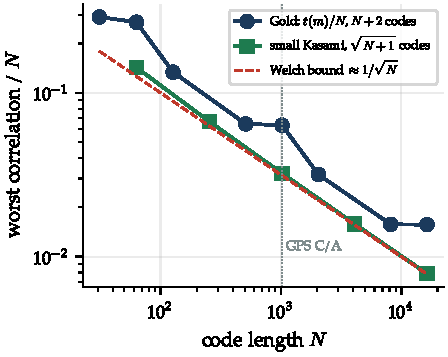
\includegraphics[width=0.5\linewidth]{figs/ch18_family_bounds}
\caption{How good can a code family be? The worst-case correlation of Gold
and small Kasami families against the Welch bound. Kasami codes sit on the bound but come in small
families; Gold codes are about $\sqrt2$ to 2 times worse but offer $N+2$ codes---1025 for the GPS
length.}\label{fig:ch18_family_bounds}\end{figure}

Random sequences have correlations of order $\sqrt N$ on average, but with occasional larger
excursions. The goal is to guarantee a maximum close to $\sqrt N$; Figure~\ref{fig:ch18_family_bounds}
shows how close the two classic families come.

\term{Gold codes} (Robert Gold, 1967) do this with trivial hardware. Take two m-sequences
$u$ and $v$ of the same degree $m$ that form a \emph{preferred pair}, meaning their
cross-correlation takes only the three values $-1$, $-t(m)$ and $t(m)-2$, where
\begin{equation}
t(m)=\begin{cases}2^{(m+1)/2}+1,&m\text{ odd},\\2^{(m+2)/2}+1,&m\text{ even, }m\not\equiv0\pmod4.\end{cases}
\end{equation}
(Preferred pairs can be constructed by decimation: $v_n=u_{qn}$ with $q=3$ for odd $m$.)
The Gold family is $\{u,\;v,\;u\oplus T^kv:\;k=0,\dots,N-1\}$, where $T^k$ is a cyclic
shift: $N+2=2^m+1$ sequences, generated by two LFSRs whose outputs are XORed, the relative
starting state selecting the family member. Every auto- and cross-correlation of the family
takes only the values $\{-1,-t(m),t(m)-2\}$ off the main peak. For $m=10$, $N=1023$ and
$t=65$: the 1025 codes of the family have cross-correlations of $-1$, $-65$ or $+63$, a
worst case of $-24$\,dB relative to the peak. This is the family GPS uses
(Figure~\ref{fig:ch18_codes}).

\term{Kasami codes} do better. The \emph{small Kasami set} for even $m$ takes an m-sequence $u$
and the shorter sequence $w$ obtained by decimating $u$ by $2^{m/2}+1$ (period
$2^{m/2}-1$), and forms $\{u,\;u\oplus T^kw\}$: $2^{m/2}$ sequences with maximum correlation
$2^{m/2}+1$, which meets the Welch bound asymptotically. The price is a small family: 32
sequences for $N=1023$. The \emph{large Kasami set} adds a third sequence to obtain a family
larger than Gold's with the same $t(m)$. Kasami sets are the benchmark against which other
families are judged; Gold codes win in practice because their family is large and
their generator is two LFSRs.

\begin{figure}[htbp]\centering
\begin{tikzpicture}[scale=0.88,transform shape,
  nd/.style={draw=navy,fill=navy!6,thick,rounded corners=2pt,font=\sffamily\scriptsize,inner sep=2pt,minimum height=0.55cm},
  bl/.style={nd,fill=gray!15,draw=gray,text=gray},
  us/.style={nd,fill=accent!15,draw=accent,text=accent!80!black},
  level distance=1.25cm]
\node[nd] (r) at (0,0) {$C_{1,0}=(1)$};
\node[us] (a) at (-3.6,-1.2) {$C_{2,0}=(1,1)$};
\node[nd] (b) at (3.6,-1.2) {$C_{2,1}=(1,-1)$};
\node[bl] (a0) at (-5.4,-2.4) {$C_{4,0}$};
\node[bl] (a1) at (-1.8,-2.4) {$C_{4,1}$};
\node[nd] (b0) at (1.8,-2.4) {$C_{4,2}=(1,-1,1,-1)$};
\node[nd] (b1) at (5.4,-2.4) {$C_{4,3}=(1,-1,-1,1)$};
\foreach \x/\n in {-6.3/0,-4.5/1,-2.7/2,-0.9/3}{\node[bl] at (\x,-3.6) {$C_{8,\n}$};}
\node[us] (c4) at (0.9,-3.6) {$C_{8,4}$};
\node[nd] (c5) at (2.7,-3.6) {$C_{8,5}$};
\node[nd] (c6) at (4.5,-3.6) {$C_{8,6}$};
\node[nd] (c7) at (6.3,-3.6) {$C_{8,7}$};
\draw[navy] (r) -- (a); \draw[navy] (r) -- (b);
\draw[gray] (a) -- (a0); \draw[gray] (a) -- (a1);
\draw[navy] (b) -- (b0); \draw[navy] (b) -- (b1);
\draw[gray] (a0) -- (-6.3,-3.3); \draw[gray] (a0) -- (-4.5,-3.3); \draw[gray] (a1) -- (-2.7,-3.3); \draw[gray] (a1) -- (-0.9,-3.3);
\draw[navy] (b0) -- (c4); \draw[navy] (b0) -- (c5); \draw[navy] (b1) -- (c6); \draw[navy] (b1) -- (c7);
\node[font=\sffamily\scriptsize,anchor=west] at (-7.0,-4.4) {SF\,8};
\node[font=\sffamily\scriptsize,text=accent!80!black,align=center] at (0,-4.5)
 {red: codes in use (a fast SF\,2 user and a slow SF\,8 user)\\grey: blocked because their ancestor is in use};
\end{tikzpicture}
\caption{The OVSF code tree. Each code spawns two children of twice the length,
$[C,C]$ and $[C,-C]$. Codes are orthogonal unless one is an ancestor of the other, so a high-rate
user (short code near the root) blocks its entire subtree---half the tree here.}
\label{fig:ch18_ovsf_tree}
\end{figure}

\begin{tryit}[Codes that ignore each other]
Open the \emph{PN, Gold and Kasami codes} experiment of Lab~25. Set \emph{Code family} to
m-sequence and \emph{Shift-register length m} to 7: the cross-correlation of the two codes has ugly
peaks. Switch to Gold and watch the histogram collapse onto just three values; then try Small
Kasami at $m=8$ and compare the ``worst cross-correlation'' readout with the theory bound.
\end{tryit}

\mdcfig{ch18_walsh}{(a) The 64 OVSF codes of spreading factor 64, black $=-1$. (b)
Orthogonal codes are orthogonal only when aligned: with even one chip of misalignment
(as multipath produces), the cross-correlation between OVSF codes is on average about
$1/\sqrt N$, but the worst pairs reach $0.4$--$0.5$ of the peak, worse than Gold codes.
Scrambling with a long PN sequence restores noise-like behaviour.}

\subsection{Orthogonal codes: Walsh--Hadamard and OVSF}

If all users are chip-synchronous, as they are on the downlink from a single base station,
one can do better than low correlation: \emph{zero} correlation. The rows of a
\term{Hadamard matrix} are mutually orthogonal $\pm1$ vectors. Sylvester's construction
builds them recursively:
\begin{equation}
H_1=[1],\qquad H_{2n}=\begin{bmatrix}H_n&H_n\\H_n&-H_n\end{bmatrix}.
\end{equation}
The rows of $H_{64}$ are the 64 \term{Walsh codes} of the IS-95 downlink. They are perfectly
orthogonal when aligned, and a user's correlator rejects all other users' signals from the
same cell completely---in the absence of multipath.

Third-generation systems needed codes of \emph{different} lengths for users with different
data rates. The \term{orthogonal variable spreading factor} (OVSF) codes of WCDMA arrange
Walsh codes in a binary tree (Figure~\ref{fig:ch18_ovsf_tree}): code $C_{n,k}$ of spreading factor
$n$ has two children, $C_{2n,2k}=[C_{n,k},\,C_{n,k}]$ and $C_{2n,2k+1}=[C_{n,k},\,-C_{n,k}]$. Any
two codes are orthogonal provided neither is an ancestor of the other. A high-rate user takes a
short code near the root and thereby blocks its whole subtree; the base station's code allocator
manages the tree like a buddy memory allocator.

Orthogonality has a fragility that Figure~\ref{fig:ch18_walsh} makes plain. Shift two Walsh
codes by even one chip relative to each other and their cross-correlation is no longer zero;
for some pairs it becomes large, because Walsh codes are highly structured (several are
periodic square waves). Multipath delays exactly such shifted copies into the receiver. That
is why every CDMA system multiplies the orthogonal channelisation code by a
\term{scrambling code}---a long PN sequence common to all users of a cell---which leaves
aligned orthogonality intact while making the misaligned interference noise-like and
Gold-code-sized.

\mdcpairany{ch18_barker}{The 11-chip Barker sequence of 802.11b has a perfect aperiodic
autocorrelation: a peak of 11 and every sidelobe 0 or $-1$, so a receiver can find each symbol's
start with a single short correlator.}{ch18_orinoco}{An ORiNOCO 802.11b PC card, typical of the
first mass-market Wi-Fi around 2000: 11\,Mchip/s direct-sequence spread spectrum at
2.4\,GHz.}

\begin{inpractice}[The code toolbox in real systems]
\begin{itemize}
\item \textbf{GPS L1 C/A}: Gold codes of length 1023 from two degree-10 LFSRs
(Section~\ref{sec:ch18:gpsca}). Modernised GPS L5 uses length-10\,230 codes built from
two 13-stage registers; L1C uses Weil codes of length 10\,230, a family with better
correlation than truncated Gold codes.
\item \textbf{IS-95/cdma2000}: 64 Walsh codes for downlink channelisation; a pair of
``short'' PN codes of period $2^{15}$ (26.67\,ms) whose phase offset (in steps of 64 chips,
512 offsets) identifies the base station; a ``long'' code of period $2^{42}-1$ (about 41
days at 1.2288\,Mchip/s) whose phase, set by a mask derived from the phone's serial number,
identifies the mobile on the uplink.
\item \textbf{WCDMA/UMTS}: OVSF channelisation codes of spreading factor 4--512; downlink
scrambling by 38\,400-chip segments of Gold codes of length $2^{18}-1$ (512 primary codes in
64 groups, identifying the cell); uplink scrambling by long Gold codes of length $2^{25}-1$
or short codes of length 256 from a quaternary sequence family (3GPP TS 25.213).
\item \textbf{802.11b}: an 11-chip Barker sequence (1 and 2\,Mb/s) and 8-chip complementary
codes (5.5 and 11\,Mb/s).
\item \textbf{LTE and 5G NR}: no CDMA spreading, but the same mathematics: the NR
pseudo-random sequence used for scrambling and reference signals is a length-31 Gold
sequence (3GPP TS 38.211, clause 5.2.1); the primary and secondary synchronisation
signals are built from m-sequences; Zadoff--Chu sequences, with ideal periodic
autocorrelation, are used for random access (Chapter~\ref{ch:sync}).
\end{itemize}
\end{inpractice}

Two further families complete the toolbox. \term{Barker sequences} have aperiodic
autocorrelation sidelobes no larger than 1 and exist only for lengths up to 13; they suit
short one-shot preambles and the 11-chip spreading of 802.11b (Figure~\ref{fig:ch18_barker}).
\term{Zadoff--Chu sequences} are complex, of constant amplitude, and have \emph{zero} periodic
autocorrelation sidelobes; they are used as channel-sounding and synchronisation sequences rather
than as data spreading codes. Both were treated in Chapter~\ref{ch:sync}.

\begin{pitfall}[Linear means predictable]
An LFSR sequence is easy to generate and easy to predict: by the Berlekamp--Massey algorithm,
$2m$ consecutive chips of an m-sequence are enough to find its polynomial and state and
generate every future chip. A code that must resist an intelligent adversary---a military
anti-jam code, the encrypted GPS P(Y) and M-codes, the scrambled timestamp sequence of
802.15.4z UWB ranging---must come from a cryptographic generator (a block cipher in counter
mode, for example), not from an LFSR. The LFSR's job is to be good at correlation, not to
keep secrets.
\end{pitfall}

%======================================================================
\section{Direct-sequence spread spectrum}
\label{sec:ch18:dsss}
%======================================================================

\subsection{Transmitter and receiver}
\mdcfig[0.98]{ch18_lab_e2}{Lab~25's \emph{DSSS against a jammer} experiment. A tone jammer
(left spectrum) towers over the spread signal; after despreading (right) it is smeared flat while
the data collapse into a narrow peak, and the constellation and error count show the link
surviving. Every control in this chapter's \emph{Try it} boxes lives in a window like this.}


Direct sequence is the workhorse: GPS, IS-95, WCDMA and the first Wi-Fi all use it. The idea
fits in one line---multiply by a fast code, then multiply by it again---and the whole of its
magic lives in what that second multiplication does to everything \emph{else} that arrives.

In \term{direct-sequence spread spectrum} (DSSS) the data waveform $d(t)=\sum_kb_k\,p_b(t-kT_b)$,
with $b_k=\pm1$, is multiplied by a spreading waveform $c(t)=\sum_nc_n\,p_c(t-nT_c)$ running
$G_p=T_b/T_c$ times faster, and the product modulates a carrier:
\begin{equation}
s(t)=\sqrt{2P}\,d(t)\,c(t)\cos(2\pi f_0t+\theta).
\label{eq:ch18:dsss}
\end{equation}
Because $d(t)c(t)$ is itself a $\pm1$ waveform with chips of duration $T_c$, the signal is
simply BPSK at the chip rate, with the $\sinc^2(fT_c)$ spectrum of
Chapter~\ref{ch:baseband}, $G_p$ times wider than the data spectrum. Quadrature versions
(QPSK spreading with different codes on I and Q, as in IS-95 and WCDMA) and pulse-shaped
chips (IS-95 and WCDMA use root-raised-cosine chip filters, with roll-off 0.22 in WCDMA)
follow the same pattern.

The receiver (Figure~\ref{fig:ch18_dsss_chain}) removes the carrier, multiplies by a locally
generated replica $c(t-\hat\tau)$ aligned with the received code, and integrates over each
bit. Because $c^2(t)=1$, an aligned replica undoes the spreading exactly:
$d(t)c(t)\cdot c(t)=d(t)$. This \term{despreading} collapses the wanted signal back to the
data bandwidth. Everything else that arrives with it---noise, interference, other users,
multipath echoes at other delays---is multiplied by $c(t)$ for the first time and is
\emph{spread}. The integrate-and-dump filter that follows passes only the data bandwidth,
about $1/T_b$, and rejects the spread-out interference outside it.

\begin{figure}[htbp]\centering
\begin{tikzpicture}[
  blk/.style={draw=navy,fill=navy!6,thick,minimum height=0.85cm,minimum width=1.05cm,align=center,font=\sffamily\scriptsize},
  mul/.style={draw=navy,circle,thick,minimum size=0.5cm,inner sep=0pt,font=\small},
  arr/.style={-{Stealth[length=2mm]},thick,navy}]
\node[blk] (src) {Data\\$b_k=\pm1$\\$R_b=1/T_b$};
\node[mul,right=0.45cm of src] (m1) {$\times$};
\node[mul,right=0.75cm of m1] (m2) {$\times$};
\node[blk,right=0.55cm of m2,fill=accent!6,draw=accent] (ch) {Channel\\$+$ jammer\\$+$ noise};
\node[mul,right=0.55cm of ch] (m3) {$\times$};
\node[mul,right=0.75cm of m3] (m4) {$\times$};
\node[blk,right=0.45cm of m4] (int) {$\int_0^{T_b}$\\dump};
\node[blk,right=0.35cm of int] (dec) {Decide\\$\hat b_k$};
\node[blk,below=0.55cm of m1] (pn1) {PN code\\$c(t)$};
\node[blk,below=0.55cm of m2] (lo1) {Carrier\\$f_0$};
\node[blk,below=0.55cm of m3] (lo2) {Carrier\\recovery};
\node[blk,below=0.55cm of m4] (pn2) {PN code\\$c(t-\hat\tau)$};
\node[blk,below=0.45cm of pn2,fill=green!6,draw=green!50!black] (sync) {Code acquisition\\and tracking};
\draw[arr] (src) -- (m1);
\draw[arr] (m1) -- (m2); \draw[arr] (m2) -- node[above,font=\scriptsize]{$s(t)$} (ch);
\draw[arr] (ch) -- node[above,font=\scriptsize]{$r(t)$} (m3); \draw[arr] (m3) -- (m4);
\draw[arr] (m4) -- (int); \draw[arr] (int) -- (dec);
\draw[arr] (pn1) -- (m1); \draw[arr] (lo1) -- (m2); \draw[arr] (lo2) -- (m3); \draw[arr] (pn2) -- (m4);
\draw[arr,green!50!black] (sync) -- (pn2);
\draw[arr,green!50!black] (int.south) |- (sync.east);
\node[font=\sffamily\scriptsize,text=navy,above=0.3cm of m1,xshift=0.6cm] {transmitter: spread};
\node[font=\sffamily\scriptsize,text=navy,above=0.3cm of m3,xshift=0.6cm] {receiver: despread};
\end{tikzpicture}
\caption{A direct-sequence spread-spectrum link. The data are multiplied by a pseudo-noise
code $G_p$ times faster than the data, then modulated onto a carrier. The receiver removes
the carrier, multiplies by a synchronised replica of the code and integrates over each bit.
Code synchronisation---first acquisition, then tracking---is the hardest part of the
receiver (Sections~\ref{sec:ch18:acq} and~\ref{sec:ch18:tracking}).}
\label{fig:ch18_dsss_chain}
\end{figure}

\subsection{Spreading does not help against white noise}
\label{sec:ch18:awgn}

Before we celebrate, an honest warning: against plain thermal noise, spreading buys exactly
nothing. Here is why, in one short calculation. Work at complex baseband with one sample per chip.
The received chips of one bit are
\begin{equation}
r_n=\sqrt{E_c}\,b\,c_n+i_n+w_n,\qquad n=0,\dots,G_p-1,
\end{equation}
where $E_c=E_b/G_p$ is the energy per chip, $w_n$ is white noise of variance $N_0$ and $i_n$
is interference. The despreader forms
\begin{equation}
z=\sum_{n=0}^{G_p-1}c_nr_n=G_p\sqrt{E_c}\,b+\sum_nc_ni_n+\sum_nc_nw_n.
\label{eq:ch18:despread}
\end{equation}
The wanted term adds coherently: its amplitude grows as $G_p$ and its power as $G_p^2$.
The noise term is a sum of $G_p$ independent terms of variance $N_0$ (multiplying white
Gaussian noise by $\pm1$ changes nothing), so its variance is $G_pN_0$. The SNR is
\begin{equation}
\frac{G_p^2E_c}{G_pN_0}=\frac{G_pE_c}{N_0}=\frac{E_b}{N_0},
\end{equation}
exactly that of the unspread signal. Spreading moved the signal energy over a wider band,
but white noise was already everywhere, so the correlator collects the same noise per unit
of signal energy as it would have without spreading. The bit error probability of DSSS-BPSK
in AWGN is $\Q(\sqrt{2E_b/N_0})$, as always. White noise is the one ``interferer'' that cannot be
diluted, because it is already as diluted as it can be.

\subsection{Narrowband interference rejection}
\label{sec:ch18:jamming}

Now the good news. Let the interference be a narrowband jammer of power $J$---say a tone
$i_n=\sqrt J\,e^{j(2\pi\nu n+\phi)}$, ten times stronger than our whole signal. An ordinary BPSK
receiver would be flattened. What does the despreader make of it?

\begin{deeper}[The jammer after despreading]
Treat the code as a sequence of independent, equally
likely $\pm1$ chips, as it effectively is for a long code. The interference term
in~\eqref{eq:ch18:despread}, $\sum_nc_ni_n$, then has zero mean and variance
\begin{equation}
\E\Big|\sum_nc_ni_n\Big|^2=\sum_n\sum_m\E[c_nc_m]\,i_ni_m^*=\sum_n|i_n|^2=G_pJ,
\end{equation}
because $\E[c_nc_m]=0$ for $n\ne m$. Whatever the jammer's waveform, the despreader turns it
into a noise-like term whose power has grown only by $G_p$, while the signal power has grown
by $G_p^2$.
\end{deeper}

With signal power $S=E_c$ per chip sample, the signal-to-interference ratio after
despreading is
\begin{equation}
\text{SIR}_{\text{out}}=\frac{G_p^2E_c}{G_pJ}=G_p\,\frac{S}{J}.
\label{eq:ch18:sirout}
\end{equation}
Equivalently, define the jammer's equivalent noise density $J_0=J/W$ spread over the
signal bandwidth $W=1/T_c$; then
\begin{equation}
\frac{E_b}{J_0}=\frac{ST_b}{J/W}=\frac{S}{J}\cdot\frac{W}{R}=G_p\,\frac{S}{J}.
\label{eq:ch18:ebj0}
\end{equation}
In words: the jammer is cut down by the processing gain. A jammer 10\,dB stronger than the signal,
facing 20\,dB of processing gain, sees its 10\,dB advantage turned into a 10\,dB deficit.

In the frequency domain (Figure~\ref{fig:ch18_jammer_spectra}), multiplying the tone by
$c(t)$ convolves its line spectrum with the code's $\sinc^2$ spectrum, smearing the jammer's
power over $\pm R_c$; the data filter of bandwidth $R_b$ passes only the fraction $1/G_p$ of
it. The receiver's despreader is the jammer's spreader.

\mdcfig{ch18_jammer_spectra}{DSSS rejection of a narrowband jammer (simulated, $G_p=63$,
$J/S=10$\,dB, long PN code). (a) Spreading widens the data spectrum by $G_p$ and lowers its
density by the same factor. (b) At the receiver a tone jammer 10\,dB stronger than the whole
signal towers over it. (c) Despreading collapses the signal back to the data bandwidth and
spreads the jammer over $\pm R_c$; inside the data filter the signal is now about 8\,dB
($G_p-J/S=18-10$\,dB) above the jammer.}

If the jammer and noise together are treated as Gaussian---a good approximation after
despreading a long code, by the central limit theorem---the bit error probability is
\begin{equation}
P_b\approx\Q\!\left(\sqrt{\frac{2E_b}{N_0+J_0}}\right)=\Q\!\left(\sqrt{\frac{2}{(E_b/N_0)^{-1}+(G_pS/J)^{-1}}}\right).
\label{eq:ch18:pbjam}
\end{equation}
Figure~\ref{fig:ch18_dsss_ber} compares this with simulation for $G_p=100$. Each curve
floors at the BER set by $E_b/J_0=G_pS/J$: with $J/S=10$\,dB the floor is at
$\Q(\sqrt{2\times10})\approx4\times10^{-6}$, whereas an unspread BPSK signal would be
destroyed by a jammer 10\,dB stronger than itself.

\begin{figure}[htbp]\centering
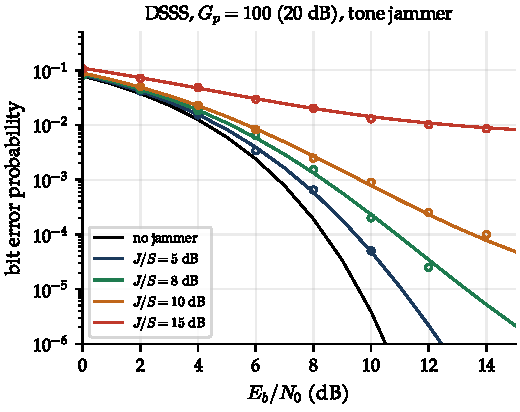
\includegraphics[width=0.49\linewidth]{figs/ch18_dsss_ber}\hfill
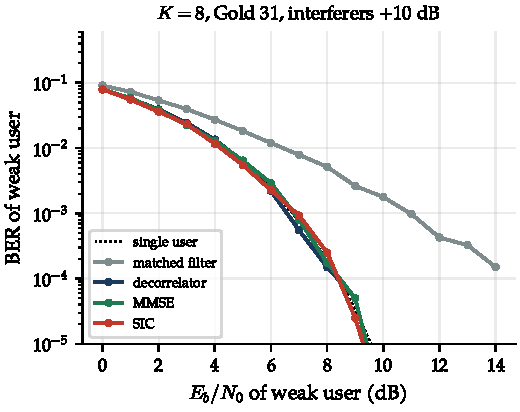
\includegraphics[width=0.49\linewidth]{figs/ch18_mud}
\caption{Left: bit error probability of DSSS-BPSK with $G_p=100$ (20\,dB) against a tone jammer
at several jammer-to-signal ratios; lines are the Gaussian approximation~\eqref{eq:ch18:pbjam},
circles simulation with a long random code. The jamming margin of this link is about
10\,dB. Right: multiuser detection (Section~\ref{sec:ch18:mud}) for a weak user among seven
synchronous interferers each 10\,dB stronger, with Gold codes of length 31.}
\label{fig:ch18_dsss_ber}
\end{figure}

\begin{tryit}[Beat the jammer]
In Lab~25's \emph{DSSS against a jammer} experiment (Figure~\ref{fig:ch18_lab_e2}), set \emph{Processing gain} to 15 and drag
\emph{Jammer-to-signal ratio J/S} up until the bit errors explode. Now change the processing gain to
255 without touching the jammer: the despread spectrum shows the jammer flattened into a carpet and
the errors vanish. Find the largest J/S each processing gain survives---that is its jamming
margin.
\end{tryit}

\subsection{Jamming margin}

The \term{jamming margin} is the jammer-to-signal ratio the link can tolerate while still
meeting its error-rate target:
\begin{equation}
M_J=G_p-\left(\frac{E_b}{J_0}\right)_{\text{req}}-L_{\text{sys}}\quad\text{(dB)},
\label{eq:ch18:mj}
\end{equation}
where $L_{\text{sys}}$ collects implementation losses. A link with 30\,dB of processing gain
that needs $E_b/J_0=10$\,dB with 2\,dB of losses has an 18\,dB jamming margin: the jammer's
received power must exceed the signal's by more than 18\,dB to break the link. Channel
coding increases the margin by lowering the required $E_b/J_0$, and since the processing
gain is fixed by bandwidth, coding gain is the cheapest jamming margin there is.

A clever jammer does not spread its power evenly. A \emph{pulsed} jammer transmits at power
$J/\rho$ for a fraction $\rho$ of the time---like a heckler who stays quiet most of the evening
and then bellows at the punchline. When it is on, the receiver sees $E_b/J_0$
reduced by the factor $\rho$; when it is off, there is no jamming at all. For uncoded DS-BPSK
the jammer's best choice is $\rho\approx0.71/(E_b/J_0)$, which produces
\begin{equation}
P_b\approx\frac{0.083}{E_b/J_0},
\end{equation}
a BER that falls only inversely with $E_b/J_0$ instead of exponentially: at
$E_b/J_0=20$\,dB, about $8\times10^{-4}$ instead of a number too small to measure
(Figure~\ref{fig:ch18_jam_strategies}a).
Partial-band jamming of frequency hopping has the same effect (Section~\ref{sec:ch18:fhss}).
The cure is forward error correction with interleaving over the jamming pulses, which turns
the few badly jammed symbols into correctable errors or erasures and restores exponential
behaviour. Every military spread-spectrum system is therefore also a coded system.

\mdcfig{ch18_jam_strategies}{Smart jammers concentrate their power. (a) A pulsed jammer against
uncoded DS-BPSK: switched on a fraction $\rho$ of the time at power $J/\rho$, it turns the
waterfall into a straight line; the worst-case $\rho$ gives $P_b\approx0.083/(E_b/J_0)$. (b) The
same game against frequency hopping with non-coherent FSK: a partial-band jammer covering a fraction
$\rho$ of the band gives, at worst, $P_b\approx0.37/(E_b/J_0)$. Coding with interleaving
restores the waterfall.}

\begin{worked}[How deep below the noise is a GPS signal?]
The GPS L1 C/A signal has a specified minimum received power of $-158.5$\,dBW
($-128.5$\,dBm) at the output of a 3\,dBi linearly polarised antenna (IS-GPS-200); take
$S=-130$\,dBm to allow for a modest antenna. A patch antenna looking at the cold sky has an
antenna temperature of roughly 100\,K, and the receiver has a 2\,dB noise figure
(170\,K), so $T_{\text{sys}}\approx270$\,K and
\[
N_0=kT_{\text{sys}}=-228.6+10\log_{10}270=-204.3\,\text{dBW/Hz}=-174.3\,\text{dBm/Hz}.
\]
The carrier-to-noise-density ratio is $C/N_0=-130+174.3=44.3$\,dB-Hz. In a
2\,MHz front-end bandwidth the noise power is $-174.3+63=-111.3$\,dBm, so the SNR before
despreading is about $-19$\,dB. The signal is invisible on a spectrum analyser.

Correlating over one code period, $T=1$\,ms, collects the signal coherently and the noise
in a bandwidth of about $1/T=1$\,kHz: the post-correlation SNR is
$(C/N_0)\,T$, or $44.3-30=14.3$\,dB. The 33\,dB improvement over the front-end SNR is the
processing gain of one code period, $10\log_{10}(2\,\text{MHz}\times1\,\text{ms})$. Integrating over a
whole 20\,ms data bit gives $E_b/N_0=44.3-10\log_{10}50=27.3$\,dB, far more than the few
decibels the navigation data need (Figure~\ref{fig:ch18_power_ladder} puts these levels on one
scale). GPS has abundant margin for its data; the margin is
spent instead on acquisition, tracking, penetration into buildings and resistance to
interference.
\end{worked}

\mdcfig[0.9]{ch18_power_ladder}{How weak is weak? Received powers on one scale. The GPS signal
arrives about 17\,dB below the thermal noise in its 2\,MHz band---like hearing a whisper across a
football stadium during a concert. After one millisecond of correlation the noise that matters
is only the noise in about 1\,kHz, and the signal stands clear of it.}

\subsection{Low probability of detection and multipath}

Two further consequences of~\eqref{eq:ch18:despread} deserve a paragraph each.

An eavesdropper without the code can only look for excess energy. The optimum detector for
an unknown noise-like signal is the \term{radiometer}, which measures power in a bandwidth
$W$ over a time $T$. The fluctuation of its noise-only output falls as $1/\sqrt{WT}$, so to
detect a signal of SNR $\gamma\ll1$ it needs roughly $WT\gtrsim(d'/\gamma)^2$, where $d'$ is a
detection index of a few. For a signal 20\,dB below the noise, $WT$ must exceed about $10^5$,
and the radiometer must know the noise level to better than $\gamma$, which is hard in
practice. A \emph{cyclostationary} detector can do better by exploiting the chip-rate and
carrier periodicities that every real DSSS signal has, which is why military LPI waveforms
use long, cryptographically generated codes and disguise their chip rate.

A signal that arrives over two paths separated by more than a chip produces two correlation
peaks, one per path. The correlator aligned with one path treats the other as interference
and suppresses it by roughly $G_p$. A spread-spectrum receiver can therefore
\emph{resolve} multipath into its components and, with several correlators, one per path,
collect the energy of all of them. Section~\ref{sec:ch18:rake} develops this Rake receiver.

\begin{inpractice}[802.11b: Barker codes and CCK]
The first widely deployed Wi-Fi was spread spectrum (Figure~\ref{fig:ch18_orinoco}).
IEEE~802.11 (1997) and 802.11b (1999) occupy channels about 22\,MHz wide in the 2.4\,GHz band at
11\,Mchip/s. At 1 and 2\,Mb/s, each DBPSK or DQPSK symbol is spread by the 11-chip Barker sequence
$+1,-1,+1,+1,-1,+1,+1,+1,-1,-1,-1$ (Figure~\ref{fig:ch18_barker}), a processing gain of 10.4\,dB.
The choice was partly regulatory: the FCC's Part~15 rules for the 2.4\,GHz ISM band then required
spread-spectrum systems to have at least 10\,dB of processing gain. For 5.5 and 11\,Mb/s, 802.11b
used \emph{complementary code keying} (CCK): each symbol is one of 16 or 256 complex 8-chip
code words at 1.375\,Msymbol/s, so the chip rate and spectrum stay the same while each
symbol carries 4 or 8 bits. CCK has almost no processing gain in the anti-jam sense; it is
really a block code with good correlation properties. In 2002 the FCC dropped the
processing-gain requirement in favour of rules that any digital modulation could meet,
which opened the band to the OFDM of 802.11g (Chapter~\ref{ch:wifi}). Wi-Fi chips still
decode the 1\,Mb/s Barker mode, because some management frames may use it.
\end{inpractice}

%======================================================================
\mdcfig{ch18_fhss}{Bluetooth hopping at 1600 hops/s over 79 channels; 25\,ms shown. (a)
Hopping over the whole band collides with a Wi-Fi network on channel 6 on roughly a quarter
of the hops (red). (b) Adaptive frequency hopping removes the 22 channels under the Wi-Fi
signal from the hop set, and the collisions disappear.}

\section{Frequency hopping}
\label{sec:ch18:fhss}
%======================================================================

Direct sequence smears the signal across the whole band at once. Frequency hopping takes the
opposite approach: it stays narrowband, but it never stays put.

\begin{analogy}[Jumping between radio stations]
Imagine two friends who want a private chat on a crowded walkie-talkie band. They agree on a
secret list of channels and a rhythm: every few hundredths of a second both jump to the next
channel on the list. An eavesdropper tuned to one channel hears a fragment of a word, then
silence. A troublemaker blasting noise on one channel spoils only the moments the friends happen
to land there. The analogy captures what hopping buys---and its weakness: unlike direct
sequence, hopping gives no protection at all for the fraction of time you land on a jammed
channel. Its protection is statistical.
\end{analogy}

In \term{frequency-hopping spread spectrum} (FHSS), the carrier frequency jumps among $N_h$
channels in a pseudo-random pattern known to the receiver, which hops its local oscillator in
synchronism. At any instant the signal is an ordinary narrowband signal, usually FSK
demodulated non-coherently, because maintaining carrier phase across hops is hard. The
spread bandwidth is $W_{ss}\approx N_hW_d$, where $W_d$ is the bandwidth of one hop, and the
processing gain is $G_p=W_{ss}/W_d=N_h$ for contiguous channels.

Hopping is classified by its speed relative to the symbol rate:
\begin{description}[style=nextline,leftmargin=1.2em,font=\sffamily\bfseries\small\color{navy}]
\item[Slow hopping.] Several symbols per hop. Simple and efficient; a jammer that finds the
current channel can destroy all the symbols of a hop, so coding and interleaving across
hops are essential. Bluetooth, GSM's optional frequency hopping and most tactical radios.
\item[Fast hopping.] Several hops per symbol. Each symbol is spread over several frequencies,
which gives frequency diversity within the symbol and defeats \emph{follower} jammers,
which must detect the frequency and retransmit on it before the hop ends. Harder to
build: the synthesiser must settle in a fraction of a symbol.
\end{description}

\mdcpairany{ch18_bt_chip}{A single-chip Bluetooth transceiver (Broadcom BCM20730) from a wireless
keyboard. Inside a few square millimetres: a synthesiser that retunes 1600 times a second, a GFSK
modem and the hop-sequence generator.}{ch18_sincgars}{A SINCGARS combat net radio. The display
reads ``Single Channel or Frequency Hopping Mode, 30--87.975\,MHz'': it hops among 25\,kHz
channels across the whole military VHF band.}

\subsection{Partial-band jamming}

Frequency hopping has no correlator gain against a jammer that sits on the channel currently
in use: that hop is simply lost. Its protection is statistical. A jammer of total power $J$
spread over a fraction $\rho$ of the hopping band has density $J_0/\rho$ there, and hits a
fraction $\rho$ of the hops. For non-coherent binary FSK, whose error probability in noise
is $\tfrac12e^{-E_b/2N_0}$, the jammed BER (ignoring thermal noise) is
\begin{equation}
P_b=\frac{\rho}{2}\exp\!\left(-\frac{\rho E_b}{2J_0}\right),
\end{equation}
and the jammer's best choice, $\rho=2/(E_b/J_0)$ (when that is less than 1), gives
\begin{equation}
P_b=\frac{e^{-1}}{E_b/J_0}\approx\frac{0.37}{E_b/J_0}.
\end{equation}
As with pulsed jamming of DSSS, the error rate falls only inversely with signal energy
(Figure~\ref{fig:ch18_jam_strategies}b).
Coding with interleaving across hops, and diversity (several hops per bit, combined),
restores exponential behaviour. The choice between DSSS and FHSS is thus not about
processing gain, which both have, but about practicalities: FHSS can spread over hundreds
of megahertz using non-contiguous channels and needs no fast chip-rate processing, while
DSSS gives coherent detection, multipath resolution and precise timing.

\begin{tryit}[Outwit a partial-band jammer]
In Lab~25's \emph{Frequency hopping} experiment choose \emph{Interference}: Partial-band jammer.
Sweep \emph{Fraction of the band jammed $\rho$} at a fixed $E_b/J_0$ of 20\,dB and find the
$\rho$ that does the most damage (it should be near $2/(E_b/J_0)=0.02$). Then raise
\emph{Hops per bit} to 3 or 5 and watch diversity take the jammer's advantage away.
\end{tryit}

\subsection{Bluetooth and adaptive hopping}

Bluetooth Classic (Basic Rate) divides the 2.4\,GHz ISM band into 79 channels of 1\,MHz,
from 2402 to 2480\,MHz, and hops once per 625\,$\mu$s time slot: 1600 hops per second (fewer
when multi-slot packets are used). The hop sequence is derived from the address and clock of
the central device of the piconet, so each piconet hops differently and piconets collide
only occasionally. All of this fits in one small chip (Figure~\ref{fig:ch18_bt_chip}). The modulation is GFSK at
1\,Mb/s, with $\pi/4$-DQPSK and 8DPSK for the
2 and 3\,Mb/s Enhanced Data Rate modes.

Hopping blindly over the whole band means that a Wi-Fi network on a 20--22\,MHz channel
spoils more than a quarter of the hops (Figure~\ref{fig:ch18_fhss}a). \term{Adaptive frequency
hopping} (AFH), introduced in Bluetooth~1.2 (2003), lets the central device classify
channels as good or bad from measured packet errors and exclude the bad ones, down to a
minimum of 20 channels, remapping their slots onto good channels. Bluetooth Low Energy uses
40 channels of 2\,MHz; three are fixed advertising channels placed in the gaps around the
common Wi-Fi channels 1, 6 and 11 (Figure~\ref{fig:ch18_ism_map}), and the other 37 carry
connections, which hop once per connection event using a channel map that excludes bad channels
(Chapter~\ref{ch:wifi}).

\mdcfig{ch18_ism_map}{The crowded 2.4\,GHz band. Wi-Fi's three non-overlapping channels 1, 6 and 11
each cover about 22\,MHz. Bluetooth Low Energy's 40 channels of 2\,MHz include three advertising
channels (red) tucked into the gaps between them, so that devices can always find each other even
in a busy office.}

\begin{inpractice}[Military hoppers]
Frequency hopping dominates military tactical radio because it can spread over bandwidths
far wider than any practical DSSS chip rate and because hopping synthesisers are cheap.
The US Army's SINCGARS VHF radio (Figure~\ref{fig:ch18_sincgars}, fielded from the late 1980s)
hops over 25\,kHz channels between 30 and 88\,MHz at roughly 100 hops per second, carrying
digitised voice and data. Link~16 (JTIDS/MIDS), the tactical data link of NATO aircraft and ships,
combines several ideas of this chapter: each 5-bit symbol is sent as one of 32 cyclic shifts of a
32-chip sequence, protected by a Reed--Solomon code, as a 6.4\,$\mu$s pulse that hops, pulse by
pulse, among 51 frequencies between 969 and 1206\,MHz (avoiding the 1030 and 1090\,MHz
secondary-radar channels), at roughly 77\,000 pulses per second. At that rate a follower
jammer must sit within a few kilometres of the path to react in time. Civil GSM also used
slow hopping (once per 4.615\,ms TDMA frame, about 217 hops/s), not for secrecy but to
average interference and fading across frequencies.
\end{inpractice}

%======================================================================
\mdcfig{ch18_access_grid}{Three ways to share a channel. (a) Frequency division and (b) time
division carve the time--frequency plane into private tiles. (c) Code division lets every user
fill the whole plane at once; the receiver tells them apart by correlating with the right code.}

\section{Code-division multiple access}
\label{sec:ch18:cdma}
%======================================================================

Picture a party where every couple speaks a different language: English in one corner, Japanese
in another, Swahili by the window. Everyone talks at once, in the same room, at the same time.
You follow your own conversation because the other languages are just babble to your ear---and
the party works as long as nobody shouts and the total din stays below what everyone can talk
over. That is \term{code-division multiple access} (CDMA), with codes for languages.

In CDMA many users transmit in the same band at the same time, each spread by its own code. Each
receiver correlates with the code it wants; the others pass through the correlator as
interference reduced by roughly $G_p$. Unlike FDMA and TDMA (Chapter~\ref{ch:multipleaccess}),
there is no hard limit on the number of users: each new user adds a little interference to
everyone else, and the system degrades gracefully until the interference is too high.

\subsection{Multiple-access interference}
Figure~\ref{fig:ch18_access_grid} sets CDMA beside its rivals. FDMA gives each user a slice of
the band, TDMA a slice of time; CDMA gives every user the whole band all the time and separates
them by code, like layers stacked on top of each other.


Consider $K$ users with codes $c^{(k)}$, received with powers $P_k$ and delays $\tau_k$. The
correlator for user 1 produces
\begin{equation}
z_1=G_p\sqrt{E_{c,1}}\,b_1+\sum_{k=2}^K\sqrt{E_{c,k}}\,b_k\,\rho_{1k}(\tau_k-\tau_1)+\nu,
\end{equation}
where $\rho_{1k}(\tau)$ is the cross-correlation of the two codes at the relative delay $\tau$
(including the effect of data transitions within the window). If the users are
\emph{synchronous} and the codes orthogonal, $\rho_{1k}=0$ and the interference vanishes:
this is the CDMA downlink from one base station, using Walsh codes. On the uplink, mobiles
at different distances arrive with arbitrary delays, orthogonality is impossible, and the
\term{multiple-access interference} (MAI) is a sum of many small random terms.

For long random codes, the \term{standard Gaussian approximation} treats the MAI as Gaussian
noise. With rectangular chips and random relative delays, each interferer of equal power
contributes a variance of $2/(3G_p)$ of the wanted signal's power (the $2/3$ comes from
averaging the chip-overlap triangle over the random chip phase), which gives Pursley's
classic result
\begin{equation}
P_b\approx\Q\!\left(\left[\frac{K-1}{3G_p}+\frac{N_0}{2E_b}\right]^{-1/2}\right).
\label{eq:ch18:sga}
\end{equation}
Read it as a sentence: each additional user adds to the effective noise as if it were a jammer of
the same power as the wanted signal, cut down by the processing gain. Ignoring thermal noise, the
effective $E_b/I_0$, where $I_0$ is the interference density, is about $G_p/(K-1)$, up to the
chip-shape factor. Nearly all of CDMA system design follows from this one ratio.

\mdcfig{ch18_nearfar_cartoon}{The near--far problem in one picture. Two phones transmit the same
power, but with fourth-power path loss the near one arrives about 49\,dB louder---far more than
any processing gain can absorb. Power control turns the near phone down until both arrive at the
same level.}

\mdcfig{ch18_nearfar}{(a) Near--far: bit error rate of a weak user with a conventional
correlator (Gold codes of length 63, random relative code phases, $E_b/N_0=8$\,dB; the dotted
line is the single-user BER) as the other users' power rises above it. A few
decibels of excess power from a handful of users already costs an order of magnitude.
(b, c) Closed-loop power control at 800 updates per second with 1\,dB steps on a Rayleigh
channel at 1.9\,GHz. At 3\,km/h the transmit power mirrors the fading and the received
power stays within about 1\,dB of target; at 60\,km/h the loop cannot keep up.}

\subsection{The near--far problem and power control}

Back at the party: what if one guest is standing right next to you, shouting? Never mind that he
speaks Finnish; at that volume he drowns out the distant whisper you are trying to follow. This
is the \term{near--far problem} (Figure~\ref{fig:ch18_nearfar_cartoon}), and in a cell it is
brutal. Equation~\eqref{eq:ch18:sga} assumed equal received powers. But a mobile near the
base station may have a path loss 60--80\,dB smaller than one at the cell edge. Its signal
arrives that much stronger, and after despreading it is still $G_p$ divided into a
much larger number. A 21\,dB processing gain cannot cope with a 60\,dB power difference
(Figure~\ref{fig:ch18_nearfar}a). It was the main technical objection to cellular CDMA in the
late 1980s.

The solution is \term{power control}: every mobile adjusts its transmit power so that all
signals arrive at the base station with the same power, the minimum needed for the target
quality. Everybody at the party agrees to speak just loudly enough to be heard, and no louder.
IS-95 uses three nested loops:
\begin{itemize}
\item \textbf{Open loop}: the mobile measures the received downlink power and sets its transmit
power so that the two sum to a constant (in dB). Fast and coarse, it handles the distance
and shadowing components, which are roughly the same on both links, but not fast fading,
because uplink and downlink are on frequencies 45\,MHz apart and fade independently.
\item \textbf{Closed loop}: the base station measures each mobile's received $E_b/I_0$ every
1.25\,ms and sends a single power-control bit, punctured into the downlink traffic channel,
telling the mobile to step its power up or down by 1\,dB. This 800\,Hz loop tracks fading
at pedestrian speeds (Figure~\ref{fig:ch18_nearfar}b). WCDMA runs the same loop at
1500\,Hz, once per slot.
\item \textbf{Outer loop}: the base station adjusts each mobile's $E_b/I_0$ target, slowly,
to hold the frame error rate at its target (typically 1\%), because the $E_b/I_0$ needed for
a given error rate depends on speed and multipath.
\end{itemize}
At vehicular speeds the fades come faster than an 800\,Hz loop with one-step, one-decibel
corrections can follow (Figure~\ref{fig:ch18_nearfar}c), and the residual fading must be
handled by interleaving, coding and Rake diversity. Power control needs a dynamic range of
about 80\,dB at the mobile. It is also why a CDMA phone (Figure~\ref{fig:ch18_cdma_phone}) is frugal: in good conditions it
transmits only milliwatts.

\begin{tryit}[Shout, then whisper]
In Lab~25's \emph{CDMA: near--far and multiuser detection} experiment
(Figure~\ref{fig:ch18_lab_e5}), keep the \emph{Detector} on
Matched filter and drag \emph{Power excess of the other users} from 0 to 20\,dB: the weak user's
constellation dissolves. Now tick \emph{Perfect power control}---everyone arrives at the same
level and the cloud snaps back. Finally untick it and try the Decorrelator instead.
\end{tryit}

\mdcpairany{ch18_cdma_vs_amps}{The worked example as a bar chart: pole capacity of an IS-95 cell
as each ingredient is added, against the six analogue channels AMPS fits into the same
1.25\,MHz.}{ch18_cdma_phone}{A cdmaOne (IS-95) handset taken apart. The metal partitions shield
the RF sections; somewhere on that board a 1.2288\,Mchip/s Rake receiver and an 80\,dB power-control
range are doing the work of this section.}

\subsection{Capacity of a CDMA cell}

How many people can talk at the party before the din wins? The capacity argument of Gilhousen,
Jacobs, Viterbi and colleagues (1991), which convinced the industry, runs as follows. With perfect
power control, each of $N$ users in a cell is received with power $S$. The interference seen by
any one of them is that of the other $N-1$, plus interference from users in neighbouring cells,
which are power-controlled by their own base stations and arrive attenuated; write it as a
fraction $f$ of the own-cell interference. Three features of the system reduce the interference
further:
\begin{itemize}
\item \textbf{Voice activity}: a speaker talks about 40\% of the time, and the IS-95 vocoder
reduces its rate (and the transmitter its power) during pauses, so each user's average
interference is multiplied by the \emph{voice activity factor} $\nu\approx0.4$.
\item \textbf{Sectorisation}: three 120$^\circ$ antennas at the base station each see only
about a third of the interferers; in practice the gain is $G_s\approx2.5$ rather than 3,
because of overlapping antenna patterns.
\item \textbf{Universal frequency reuse}: every cell uses the same carrier (reuse factor 1),
which is already reflected in $f$.
\end{itemize}
The bit energy to interference density ratio is then
\begin{equation}
\frac{E_b}{I_0}=\frac{S/R}{\big[(N-1)\nu S(1+f)/G_s\big]/W+N_0}.
\end{equation}
Neglecting thermal noise and solving for $N$:
\begin{equation}
N\approx1+\frac{W/R}{E_b/I_0}\cdot\frac{G_s}{\nu\,(1+f)}.
\label{eq:ch18:capacity}
\end{equation}
In words: capacity is the processing gain divided by the $E_b/I_0$ each user needs, boosted by
silence and sectors, and taxed by the neighbours. Compare FDMA or TDMA, whose capacity is the
number of channels divided by the reuse factor (7 in AMPS). CDMA's capacity is set instead by the
required $E_b/I_0$, which is why the battle for CDMA capacity was fought with better vocoders,
Rake receivers, coding and power control.

\mdcfig{ch18_capacity}{(a) Uplink pole capacity of an IS-95 cell from~\eqref{eq:ch18:capacity},
showing how each ingredient changes the number of users. (b) Soft capacity: with Poisson call
arrivals, random voice activity and fluctuating other-cell interference, the probability that
the total interference exceeds the budget rises smoothly with load, rather than abruptly at a
fixed number of channels. Operators trade a slightly higher outage probability for more users
at busy hours.}

\begin{worked}[IS-95 uplink capacity]
IS-95 uses $W=1.2288$\,Mchip/s and $R=9.6$\,kb/s, so $W/R=128$ (21.1\,dB). With the
convolutional code, interleaving and Rake reception, the uplink needs roughly
$E_b/I_0=7$\,dB (a factor of 5.0) for a 1\% frame error rate. A single isolated omni cell
with continuously active users would carry
\[
N=1+128/5.0\approx26\text{ users}.
\]
Voice activity ($\nu=0.4$) multiplies the interference-limited term by 2.5, giving 65.
Other-cell interference with $f=0.55$, a typical value for a hexagonal layout with
fourth-power path loss, divides it by 1.55, giving 42. Three sectors with $G_s=2.55$ multiply
it again, giving about 105 users per cell, or 35 per sector, on a 1.25\,MHz carrier
(Figures~\ref{fig:ch18_capacity}a and~\ref{fig:ch18_cdma_vs_amps}). An AMPS system
(Chapter~\ref{ch:cellular}) with 30\,kHz channels and a seven-cell reuse pattern puts
$1250/30/7\approx6$ analogue voice channels per cell into the same spectrum. Gilhousen and
colleagues claimed a capacity gain over analogue of roughly an order of magnitude or more. Real
networks, which run at perhaps 50--75\% of this pole capacity to keep the noise rise in check and
suffer imperfect power control, achieved less, but a gain of several times over AMPS and about two
to three times over the digital TDMA of IS-54 was widely reported.
\end{worked}

\begin{figure}[htbp]\centering
\begin{tikzpicture}[
  bs/.style={draw=navy,thick,fill=navy!8,minimum width=1.1cm,minimum height=0.7cm,font=\sffamily\scriptsize,align=center},
  arr/.style={-{Stealth[length=2mm]},thick}]
\node[bs] (A) at (0,0) {cell A};
\node[bs] (B) at (9,0) {cell B};
\draw[navy!30,thick,dashed] (0,0) circle (2.6cm);
\draw[green!40!black!30,thick,dashed] (9,0) circle (2.6cm);
\foreach \x/\l in {2.0/1,4.5/2,7.0/3}{\node[draw=accent,fill=accent!15,thick,minimum width=0.35cm,minimum height=0.6cm] (m\l) at (\x,-1.6) {};}
\draw[arr,navy] (A) -- (m1); \draw[arr,navy] (A) -- (m2); \draw[arr,green!40!black] (B) -- (m2); \draw[arr,green!40!black] (B) -- (m3);
\node[font=\sffamily\scriptsize,align=center] at (2.0,-2.4) {active set: A};
\node[font=\sffamily\scriptsize,align=center,text=accent] at (4.5,-2.55) {active set: A and B\\Rake combines both;\\obeys either's ``power down''};
\node[font=\sffamily\scriptsize,align=center] at (7.0,-2.4) {active set: B};
\draw[-{Stealth},gray,thick] (1.2,-3.3) -- node[below,font=\sffamily\scriptsize]{mobile moves from A to B: make before break} (7.8,-3.3);
\end{tikzpicture}
\caption{Soft handoff. Because every cell uses the same carrier, a mobile between two cells talks
to both at once: its Rake receiver combines both downlinks, and on the uplink the network keeps
the better frame. Cell B is added to the active set when its pilot rises above T\_ADD and cell A is
dropped when its pilot falls below T\_DROP.}
\label{fig:ch18_soft_handoff}
\end{figure}

The capacity formula hides a subtlety that operators came to value: \term{soft capacity}.
An FDMA or TDMA cell with 30 channels blocks the 31st call. A CDMA cell admits another user
at the cost of a little more interference for everyone; capacity is a statistical limit set
by the probability that the instantaneous interference exceeds the budget
(Figure~\ref{fig:ch18_capacity}b). A lightly loaded neighbour contributes less interference,
so a busy cell can borrow capacity from quiet neighbours. The flip side is \emph{cell
breathing}: as load rises, the noise floor rises, the cell edge shrinks and the coverage
area contracts---the party gets louder, so you can no longer hear people at the far end of the
room. The uplink \term{noise rise} $\eta$ of a cell loaded to a fraction $x$ of its
pole capacity is $1/(1-x)$; at 75\% load it is 6\,dB, which must be included in every link
budget (Chapter~\ref{ch:channels}).

\subsection{Soft handoff}

Because every cell uses the same frequency, a mobile can talk to two or three base stations
at once (Figure~\ref{fig:ch18_soft_handoff}). In \term{soft handoff}, the mobile continuously measures the pilot strength $E_c/I_0$
of all nearby cells. When a pilot rises above a threshold (T\_ADD), the network adds that
base station to the mobile's \emph{active set}; when it falls below another (T\_DROP) for
a few seconds, it is removed. On the downlink, the mobile combines the signals from all
members of the active set in its Rake receiver. On the uplink, each base station decodes the
mobile independently and the network selects the best frame. A mobile in soft handoff
obeys a power-down command from \emph{any} base station, so it always transmits the minimum
power needed by the best one. Soft handoff provides macro-diversity against shadowing, a gain
of several decibels at the cell edge, and it removes the ``ping-pong'' and dropped calls of
hard handoff---it is ``make before break'' rather than ``break before make''. Its cost is that
one call occupies channel resources at several base stations; typically 30--50\% of IS-95 calls
were in soft handoff at any time.

\begin{figure}[htbp]\centering
\begin{tikzpicture}[
  blk/.style={draw=navy,fill=navy!6,thick,minimum height=0.7cm,minimum width=1.2cm,align=center,font=\sffamily\scriptsize},
  mul/.style={draw=navy,circle,thick,minimum size=0.48cm,inner sep=0pt,font=\small},
  arr/.style={-{Stealth[length=2mm]},thick,navy}]
\node[blk] (in) {Received\\chips $r_n$};
\node[blk,right=0.9cm of in,yshift=1.2cm] (d1) {Delay $\tau_1$};
\node[blk,right=0.9cm of in] (d2) {Delay $\tau_2$};
\node[blk,right=0.9cm of in,yshift=-1.2cm] (d3) {Delay $\tau_3$};
\foreach \i in {1,2,3}{
  \node[blk,right=0.45cm of d\i] (c\i) {Despread\\$\sum c_n(\cdot)$};
  \node[mul,right=0.45cm of c\i] (w\i) {$\times$};
  \node[font=\scriptsize,above=0.05cm of w\i] {$\hat h_\i^*$};
  \draw[arr] (in.east) -- ++(0.35,0) |- (d\i.west);
  \draw[arr] (d\i) -- (c\i); \draw[arr] (c\i) -- (w\i);
}
\node[draw=navy,circle,thick,minimum size=0.6cm,right=0.8cm of w2] (sum) {$\Sigma$};
\foreach \i in {1,2,3}{\draw[arr] (w\i) -- (sum);}
\node[blk,right=0.45cm of sum] (dec) {Decide\\$\hat b$};
\draw[arr] (sum) -- (dec);
\node[blk,below=0.55cm of d3,xshift=1.0cm,fill=green!6,draw=green!50!black,minimum width=3.4cm] (srch) {Searcher: pilot correlation over\\delay; assigns fingers, estimates $\hat h_l$};
\draw[arr,green!50!black] (in.south) |- (srch.west);
\draw[arr,green!50!black,dashed] (srch.north) -- (d3.south);
\draw[arr,green!50!black,dashed] (srch.east) -| (w3.south);
\end{tikzpicture}
\caption{A three-finger Rake receiver. Each finger despreads the received signal at the delay
of one resolvable path, found by the searcher; the finger outputs are weighted by the
conjugates of the estimated path gains (maximal-ratio combining) and summed. In IS-95 and
WCDMA phones the channel estimates come from the pilot channel, and the same structure
combines signals from different base stations during soft handoff.}
\label{fig:ch18_rake_rx}
\end{figure}

\begin{history}[Qualcomm and the CDMA wars]
In 1985 Irwin Jacobs, Andrew Viterbi and five colleagues founded Qualcomm in San Diego. Jacobs
and Viterbi had previously built Linkabit, a successful military satellite and spread-spectrum
communications company, and Viterbi had invented the Viterbi algorithm
(Chapter~\ref{ch:classiccodes}). Qualcomm's first product was OmniTRACS, a satellite messaging
and positioning system for trucks. In 1988--89 Klein Gilhousen, Jacobs and Viterbi proposed
CDMA for cellular telephony---just as the Cellular Telecommunications Industry Association
had chosen TDMA (IS-54) as the US digital standard.

The reaction from much of the industry was scepticism bordering on hostility. Critics argued
that the near--far problem made CDMA impractical, that power control could not work to the
precision required, and that the capacity claims were fantasy. Qualcomm demonstrated a
working system in San Diego in 1989 and ran field trials with operators, including a
well-publicised trial in New York. The TIA published the CDMA air interface as interim
standard IS-95 in 1993. Hutchison launched the first commercial network in Hong Kong in
1995, and South Korea, which had chosen CDMA as its national standard, launched in early
1996 and became for a time the largest CDMA market in the world. In the US, CDMA was adopted
by Verizon's predecessors and Sprint. The ``CDMA wars'' did not end with a single winner---GSM's
TDMA dominated the world in the 2G era---but all three main 3G standards (WCDMA, cdma2000 and
China's TD-SCDMA) were built on CDMA, and the patents made Qualcomm one of the world's largest
semiconductor and licensing companies.
\end{history}

%======================================================================
\section{The Rake receiver}
\label{sec:ch18:rake}
%======================================================================

In a city, your phone never receives just one copy of the signal. It receives the direct wave,
then an echo off the office block across the street a microsecond later, then another off the
hill behind. To a narrowband receiver those echoes are a curse: they add up with random phases and
the signal fades. To a spread-spectrum receiver they are a gift---extra copies of the same
message, each one separately recognisable because the code's sharp correlation peak tells them
apart.

\mdcfig{ch18_rake}{(a) The searcher's view: the magnitude of the pilot correlation against
delay for a three-path channel at a WCDMA-like chip rate, with fingers assigned to the three
peaks. (b) BER of BPSK with an $L$-finger maximal-ratio Rake in independent Rayleigh paths of
equal power, total received energy fixed; lines from~\eqref{eq:ch18:rakeber}, circles
simulation. The diversity order equals the number of resolvable paths.}

\begin{analogy}[A garden rake gathering the echoes]
Drag a garden rake across a lawn and each tine gathers the leaves in its own strip; together they
collect far more than a single stick could. A Rake receiver gives each strong echo its own
``tine'', a correlator set to exactly that echo's delay, and then sweeps the results together.
Echoes that would have cancelled each other in a simple receiver now add up. The analogy's limit:
real tines are evenly spaced, but a Rake's fingers go wherever the echoes happen to be, and a
searcher keeps moving them as the echoes drift.
\end{analogy}

A wideband signal in a multipath channel arrives as a sum of delayed copies
(Chapter~\ref{ch:channels}),
\begin{equation}
r(t)=\sum_{l=1}^{L}h_l\,s(t-\tau_l)+n(t).
\end{equation}
If the delays differ by more than a chip, a correlator aligned with path $l$ sees that path
coherently and the others as interference suppressed by $G_p$. Each such correlator is a
\term{finger}. The \term{Rake receiver} of Price and Green (1958) assigns a finger to each
strong path, weights the finger outputs and adds them, gathering the energy of all the paths
like the tines of a garden rake gathering leaves (Figure~\ref{fig:ch18_rake_rx}). With finger
outputs $z_l=h_l\sqrt{E_b}\,b+\nu_l$, the optimum combination is \term{maximal-ratio
combining}:
\begin{equation}
z=\sum_{l=1}^Lh_l^*z_l=\sqrt{E_b}\,b\sum_l|h_l|^2+\sum_lh_l^*\nu_l,
\qquad
\gamma_{\text{Rake}}=\frac{E_b}{N_0}\sum_{l=1}^L|h_l|^2=\sum_l\gamma_l.
\label{eq:ch18:mrc}
\end{equation}
The output SNR is the \emph{sum} of the finger SNRs: multipath, which is destructive to a
narrowband receiver, becomes a source of diversity. Strong fingers get big weights, weak ones
small, and the conjugate $h_l^*$ rotates every echo back into phase before they are added.


\mdcfig[0.55]{ch18_rake_snr}{Diversity, seen directly (simulated). The distribution of the
combined SNR for one, two and four equal Rayleigh paths at the same 10\,dB mean. Deep fades below
3\,dB happen 18\% of the time with one finger and about 1\% with four.}

If the $L$ paths fade independently with Rayleigh statistics and equal mean power, the BER of
coherent BPSK with MRC is
\begin{equation}
P_b=\left(\frac{1-\mu}{2}\right)^L\sum_{k=0}^{L-1}\binom{L-1+k}{k}\left(\frac{1+\mu}{2}\right)^k,
\qquad\mu=\sqrt{\frac{\bar\gamma_c}{1+\bar\gamma_c}},
\label{eq:ch18:rakeber}
\end{equation}
where $\bar\gamma_c$ is the mean SNR per path. At high SNR it falls as $\bar\gamma^{-L}$: the
diversity order is the number of resolvable paths. Figure~\ref{fig:ch18_rake} shows the
effect, with the total energy held constant: two fingers save about 15\,dB at a BER of
$10^{-4}$, and four save about 21\,dB, compared with a single Rayleigh path.
Figure~\ref{fig:ch18_rake_snr} shows where that saving comes from: with more fingers the
combined SNR almost never collapses, because all the echoes rarely fade at once.

\begin{tryit}[Rake the echoes]
In Lab~25's \emph{The RAKE receiver}, set \emph{Resolvable paths} to 3 and \emph{RAKE fingers}
to 1: the BER is stuck on the Rayleigh line. Add fingers one at a time and watch the curve steepen.
Then switch \emph{Combining} from Maximal ratio to Equal gain and Selection, and measure what each
shortcut costs in decibels at a BER of $10^{-3}$.
\end{tryit}

Three practical points complete the picture. First, the paths must be resolvable: two
paths closer than about one chip merge into one finger that fades. A 1.2288\,Mchip/s IS-95
signal resolves delays of about 0.8\,$\mu$s (240\,m of path difference), which is enough in
suburban and urban macrocells but not indoors; 3.84\,Mchip/s WCDMA resolves 0.26\,$\mu$s.
Second, the fingers need channel estimates $\hat h_l$, which is why every CDMA downlink has a
continuous pilot channel (Walsh code 0 in IS-95) and the uplinks of the 3G systems added
pilot symbols. Third, the Rake is matched only to the paths, not to the interference: in
heavy multipath on the downlink, the multipath copies destroy the Walsh orthogonality
(Figure~\ref{fig:ch18_walsh}), and a chip-level \emph{equaliser}
(Chapter~\ref{ch:equalization}) that restores it outperforms the Rake. HSDPA terminals use
such equalisers.

\mdcfig[0.55]{ch18_mud_scatter}{What multiuser detection buys (simulated: three misaligned Gold-31
interferers, each 6\,dB stronger than the weak user). The matched filter's output for the weak
user is smeared into several humps by the interferers and straddles the threshold; the decorrelator
removes them and leaves two clean, well-separated peaks.}

\begin{keyidea}[A Rake is a matched filter for the channel]
The Rake combiner, with fingers at every chip delay and weights $h_l^*$, is exactly the filter
matched to the received pulse $\sum_lh_lc(t-\tau_l)$, the matched filter of
Chapter~\ref{ch:baseband} applied to the combined code-and-channel response. Spreading is what
makes this matched filter useful: the code's sharp autocorrelation keeps the fingers from
interfering with one another. OFDM (Chapter~\ref{ch:ofdm}) solves the same multipath problem
in the frequency domain, at lower complexity for wide bandwidths, which is the main reason
4G abandoned CDMA.
\end{keyidea}

%======================================================================
\mdcfig[0.98]{ch18_lab_e5}{Lab~25's \emph{CDMA: near--far and multiuser detection} with six users,
the other five arriving 5\,dB stronger than the weak one. The matched filter's decision statistic
(bottom right) is smeared by multiple-access interference into two humps, and the weak user's
error rate is about 50 times what it would be alone in the cell. Switch the \emph{Detector} menu
to the decorrelator, MMSE or SIC to see them pulled apart.}

\section{Multiuser detection}
\label{sec:ch18:mud}
%======================================================================

The conventional CDMA receiver treats other users' signals as noise. But that is a strange thing
to do at a base station, which knows everyone's code, timing and power! It is like a referee who
can hear every player but insists on listening to one at a time. A receiver that detects them
jointly can do much better. This is \term{multiuser detection} (MUD), the subject of Sergio
Verd\'u's work in the 1980s.

Write the synchronous $K$-user system in vector form. Stack one symbol period of chips:
\begin{equation}
\vect y=\vect S\vect A\vect b+\vect n,
\end{equation}
where the columns of $\vect S$ ($G_p\times K$) are the unit-energy codes, $\vect A$ is the
diagonal matrix of amplitudes, $\vect b$ the vector of symbols and $\vect n$ white noise of
variance $\sigma^2$ per chip. The bank of matched filters produces
$\vect z=\vect S^{\mathsf T}\vect y=\vect R\vect A\vect b+\vect S^{\mathsf T}\vect n$, where
$\vect R=\vect S^{\mathsf T}\vect S$ is the code cross-correlation matrix. Then:
\begin{description}[style=nextline,leftmargin=1.2em,font=\sffamily\bfseries\small\color{navy}]
\item[Conventional detector.] $\hat{\vect b}=\operatorname{sgn}(\vect z)$. Ignores $\vect R$;
suffers from MAI and the near--far problem.
\item[Optimum detector.] Maximum-likelihood over all $2^K$ symbol vectors (Verd\'u, 1986).
Exponential in $K$; a benchmark, not a product.
\item[Decorrelator.] $\hat{\vect b}=\operatorname{sgn}(\vect R^{-1}\vect z)$. Removes the
MAI completely, whatever the interferers' powers---it is \emph{near--far resistant}---at
the cost of enhancing the noise, exactly like the zero-forcing equaliser of
Chapter~\ref{ch:equalization}.
\item[MMSE detector.] $\hat{\vect b}=\operatorname{sgn}\big((\vect R+\sigma^2\vect
A^{-2})^{-1}\vect z\big)$. Balances MAI suppression against noise enhancement; it tends to
the decorrelator at high SNR and to the conventional detector at low SNR.
\item[Successive interference cancellation (SIC).] Detect the strongest user, regenerate its
signal, subtract it, and repeat with the next strongest. Simple and effective when the powers
are unequal, which is exactly the near--far case; errors in early stages propagate. At the party,
it is like politely asking the loudest guest to repeat himself, writing down what he said, and
mentally deleting him so you can hear the next.
\end{description}
Figure~\ref{fig:ch18_mud_scatter} shows the difference directly.

In Figure~\ref{fig:ch18_dsss_ber} (right), seven interferers 10\,dB stronger than the wanted
user leave the conventional detector two orders of magnitude worse at 10\,dB, while the
decorrelator, MMSE and SIC receivers are close to the single-user bound.

\begin{table}[htbp]\centering\small
\caption{CDMA cellular air interfaces compared (main parameters; later releases added many
options).}
\label{tab:ch18:cdma}
\begin{tabularx}{\linewidth}{@{}l X X X@{}}
\toprule
& IS-95 (cdmaOne) & cdma2000 1x / EV-DO & WCDMA (UMTS) / HSPA\\
\midrule
Chip rate & 1.2288\,Mchip/s & 1.2288\,Mchip/s & 3.84\,Mchip/s\\
Carrier spacing & 1.25\,MHz & 1.25\,MHz & 5\,MHz\\
Base-station sync & GPS-synchronous & GPS-synchronous & asynchronous\\
Cell identity & short-PN code offset (512) & short-PN code offset & 512 scrambling codes\\
Channelisation & 64 Walsh codes & Walsh codes, variable length & OVSF, SF 4--512\\
Uplink modulation & 64-ary Walsh orthogonal, non-coherent & BPSK with pilot (coherent) & BPSK, I/Q multiplexed data/control\\
Power control & 800\,Hz & 800\,Hz & 1500\,Hz\\
Frame & 20\,ms & 20\,ms; EV-DO 1.67\,ms slots & 10\,ms (15 slots); HSPA 2\,ms\\
Coding & convolutional & convolutional, turbo & convolutional, turbo\\
Peak data rate (downlink) & 14.4\,kb/s & 153\,kb/s (1x); 2.4--3.1\,Mb/s (EV-DO) & 2\,Mb/s (R99); 14.4\,Mb/s (HSDPA) and beyond\\
\bottomrule
\end{tabularx}
\end{table}

\begin{figure}[htbp]\centering
\begin{tikzpicture}[
  st/.style={draw=navy,thick,fill=navy!6,rounded corners=2pt,minimum height=1.25cm,text width=3.3cm,align=center,font=\sffamily\scriptsize},
  arr/.style={-{Stealth[length=2.2mm]},thick,navy}]
\node[st] (a) at (0,0) {\textbf{Step 1: slot timing}\\correlate with the primary sync code, the same in every cell};
\node[st,fill=green!8,draw=green!50!black] (b) at (4.3,0) {\textbf{Step 2: frame timing and code group}\\read the secondary sync code pattern (64 groups)};
\node[st,fill=accent!8,draw=accent] (c) at (8.6,0) {\textbf{Step 3: scrambling code}\\try the 8 codes of the group on the pilot channel};
\draw[arr] (a) -- (b); \draw[arr] (b) -- (c);
\node[font=\sffamily\scriptsize,text=navy!70] at (0,-1.0) {666.7\,$\mu$s slot found};
\node[font=\sffamily\scriptsize,text=green!40!black] at (4.3,-1.0) {10\,ms frame, 1 of 64 groups};
\node[font=\sffamily\scriptsize,text=accent] at (8.6,-1.0) {1 of 512 cells identified};
\end{tikzpicture}
\caption{How a WCDMA phone finds a cell without GPS-synchronised base stations: a three-step search
that narrows 512 possible scrambling codes, at unknown timing, to one, by solving for slot timing,
then frame timing and code group, then the code itself.}
\label{fig:ch18_wcdma_search}
\end{figure}

\begin{inpractice}[Where multiuser detection went]
Full multiuser detection was too complex for the IS-95 and early WCDMA base stations, but
its ideas spread. WCDMA and cdma2000 base stations later added interference cancellation for
high-rate uplink users; the GSM-era ``single antenna interference cancellation'' and
LTE's interference-rejection combining use the MMSE idea across antennas rather than codes;
and SIC is the decoding rule behind non-orthogonal multiple access (NOMA), which superposes
users in power and separates them at the receiver (Chapter~\ref{ch:multipleaccess}). MIMO
detection (Chapter~\ref{ch:mimo}) is the same mathematics with antennas in place of codes:
$\vect y=\vect H\vect x+\vect n$, solved by zero forcing, MMSE or successive cancellation.
\end{inpractice}

%======================================================================
\section{CDMA in third-generation cellular}
\label{sec:ch18:3g}
%======================================================================

By the late 1990s the CDMA wars had been won, at least for 3G: the ITU's IMT-2000 standards were
all CDMA. Their parameters are compared in Table~\ref{tab:ch18:cdma}; their history and network
architecture are in Chapter~\ref{ch:cellular}.

\paragraph{WCDMA.} The European and Japanese 3G standard, specified by 3GPP from 1999, uses
3.84\,Mchip/s in 5\,MHz carriers with root-raised-cosine chips of roll-off 0.22. Data are
spread by an OVSF channelisation code and then scrambled by a cell-specific Gold code
(downlink) or a user-specific code (uplink), as in TS~25.213. The spreading factor sets the
rate: SF~4 carries 960\,ksymbol/s, SF~256 carries 15\,ksymbol/s. Base stations are not
synchronised, so a phone finds a cell with a three-step search
(Figure~\ref{fig:ch18_wcdma_search}): slot timing from the primary
synchronisation code (identical in all cells), frame timing and the scrambling-code group
from the secondary synchronisation codes, then the scrambling code itself by correlating with
the eight candidates of the group on the pilot channel. Release~5's HSDPA (2002) moved
towards the 4G design: a shared downlink channel using up to 15 codes of SF~16, 16-QAM
(later 64-QAM and MIMO), 2\,ms frames, fast scheduling at the base station and hybrid ARQ.

\paragraph{cdma2000.} The evolution of IS-95 kept its 1.2288\,Mchip/s chip rate and
GPS-synchronised base stations, added coherent uplink detection with a pilot, turbo codes and
variable-length Walsh codes. \emph{EV-DO} (1xEV-DO, ``evolution--data optimised'') turned the
downlink into a time-multiplexed channel transmitted at full power to one user at a time,
with the rate chosen from the user's channel quality report every 1.67\,ms slot---the first
widely deployed opportunistic scheduler, an idea that became central in LTE.

\begin{pitfall}[GPS-synchronised networks and their single point of failure]
IS-95 and cdma2000 base stations identify themselves by the phase of a common short PN
code, which works only if every base station knows absolute time to within a few
microseconds. Every cdmaOne and cdma2000 base station therefore had a GPS receiver, and
CDMA networks were among the first critical infrastructure to depend on GNSS. A base station
that lost GPS ran on a holdover oscillator for hours to days before its timing drifted
too far. Section~\ref{sec:ch18:vulnerability} returns to the dependence of modern networks on
GNSS time, which has only grown with 4G and 5G TDD (Chapter~\ref{ch:sync}).
\end{pitfall}

%======================================================================
\section{Chirp spread spectrum and ultra-wideband}
\label{sec:ch18:css}
%======================================================================

Two more ways to spend bandwidth have found enormous modern markets: chirps, which let a
battery-powered sensor reach a gateway kilometres away, and ultra-short pulses, which let your
phone find your keys to within a few centimetres.

\mdcpairany{ch18_chirp}{Pulse compression. A chirp sweeping a bandwidth $B$ over a time $T$ (top)
emerges from its matched filter as a pulse about $1/B$ wide (bottom): all the energy of the long
chirp, the timing sharpness of a short pulse.}{ch18_lora_tradeoff}{LoRa's trade at 125\,kHz with the
rate-4/5 code: each step up in spreading factor roughly doubles the time on air of a 20-byte packet
(bars, bit rates printed above) and buys about 2.5\,dB of sensitivity (red, approximate).}

\subsection{Chirps and LoRa}

A \term{chirp} is a sinusoid whose frequency sweeps linearly across a bandwidth $B$ in a time
$T$---the ``whoop'' of a slide whistle. Its matched filter compresses it into a pulse of width
about $1/B$, a gain of $BT$ (Figure~\ref{fig:ch18_chirp}); radar engineers have used this
\emph{pulse compression} since the 1950s to obtain the range resolution of a short pulse with the
energy of a long one. A chirp is also remarkably robust to Doppler and to oscillator offsets: a
frequency offset merely shifts the compressed peak slightly in time.

\term{LoRa}, a proprietary physical layer developed by the French start-up Cycleo and acquired by
Semtech in 2012, uses chirps for low-power, long-range IoT links (Chapter~\ref{ch:wifi}). A
symbol is an up-chirp of $2^{SF}$ chips across a bandwidth $B$ (125, 250 or 500\,kHz),
cyclically shifted in frequency by one of $2^{SF}$ amounts; the \emph{spreading factor}
$SF=7,\dots,12$ sets the number of bits per symbol. The demodulator multiplies by a
down-chirp (``dechirping''), which turns each symbol into a constant tone whose frequency is
the shift, and takes an FFT of size $2^{SF}$: the peak bin is the symbol
(Figure~\ref{fig:ch18_css_uwb}a,b). This is non-coherent $M$-ary orthogonal signalling with
$M=2^{SF}$, and like all orthogonal signalling (Chapter~\ref{ch:modulation}) it trades
bandwidth for power efficiency. The symbol time is $2^{SF}/B$ and the bit rate
$SF\cdot B/2^{SF}$ times the code rate: at SF\,12 and 125\,kHz, 366\,b/s before coding (293\,b/s
with the rate-4/5 code), and the link works at an SNR of about $-20$\,dB in the channel bandwidth,
giving sensitivities near $-137$\,dBm. Each step in SF roughly doubles the time on air and buys
about 2.5\,dB (Figure~\ref{fig:ch18_lora_tradeoff}).

\mdcfig{ch18_css_uwb}{(a) A LoRa SF7 frame: preamble up-chirps followed by data symbols, each a
cyclically shifted chirp. (b) Dechirping and a 128-point FFT recover symbol 37 at an SNR of
$-10$\,dB in the channel bandwidth. (c) A Gaussian monocycle and a carrier-modulated
802.15.4z pulse (channel 5). (d) Their spectra, scaled to the FCC indoor limit of
$-41.3$\,dBm/MHz: the baseband monocycle violates the stricter limits below 3.1\,GHz,
whereas the modulated pulse sits comfortably inside the UWB band.}

\subsection{Ultra-wideband impulse radio}

At the other extreme, \term{ultra-wideband} (UWB) radio spreads by using very short pulses.
The FCC's 2002 rules defined UWB as a signal with a bandwidth of at least 500\,MHz or a
fractional bandwidth of at least 20\%, and allowed it to transmit, unlicensed, between 3.1
and 10.6\,GHz at an average EIRP density of no more than $-41.3$\,dBm/MHz---the same limit as
unintentional emissions from any electronic device. Over 500\,MHz that is about $-14$\,dBm,
less than 0.05\,mW. UWB lives \emph{under} everyone else's noise floor, a ghost in the spectrum.

\mdcpairany{ch18_lora_gw}{An outdoor LoRaWAN gateway for the 868\,MHz band. One such box, with a
mast-mounted antenna, can collect readings from thousands of meters and sensors over several
kilometres.}{ch18_airtag}{A UWB tag on a key ring. Item finders and digital car keys use 802.15.4z
ultra-wideband ranging to locate a device to within roughly ten centimetres.}

The original impulse-radio idea (Win and Scholtz, 1990s) used baseband pulses such as
Gaussian monocycles, time-hopped to allow multiple access. Such pulses have energy at low
frequencies, where the masks are strict (Figure~\ref{fig:ch18_css_uwb}c,d), so practical
systems use pulses modulated onto a carrier. IEEE 802.15.4a (2007) and 802.15.4z (2020)
define \emph{high-rate pulse} (HRP) UWB with channels about 500\,MHz wide (channel 5 at
6.5\,GHz and channel 9 at 8\,GHz are the common ones), bursts of pulses at a mean pulse
repetition frequency of tens of megahertz, and a preamble of ternary sequences with perfect
periodic autocorrelation.

Its killer application is ranging. Two devices exchange messages and timestamp their
arrival (\emph{two-way ranging}); the round-trip time, minus the known reply delay, gives the
distance. With 500\,MHz of bandwidth the leading edge of the channel impulse response can be
found to within a few centimetres, and, crucially, the first path can be separated from later
reflections. 802.15.4z added the \emph{scrambled timestamp sequence} (STS), a
cryptographically generated pulse sequence that an attacker cannot predict, to stop
distance-reduction attacks in which a relay or a spoofer makes a car key appear closer than
it is. Apple's U1 chip (iPhone~11, 2019), Samsung's and Google's phones, and the Car
Connectivity Consortium's Digital Key~3.0 use HRP UWB for precise device finding and
keyless car entry (Figure~\ref{fig:ch18_airtag}). LoRa's niche is the opposite one: a single
gateway (Figure~\ref{fig:ch18_lora_gw}) collecting tiny readings from far away.

\begin{worked}[Ranging resolution from bandwidth]
A UWB pulse with 500\,MHz bandwidth has a duration of roughly 2\,ns, corresponding to
$c\times2\,\text{ns}=60$\,cm. Two paths closer than about this distance merge. But the
\emph{accuracy} with which the arrival time of a single clean path can be measured is
set by the SNR as well as the bandwidth. The Cram\'er--Rao bound for delay
(Chapter~\ref{ch:sync}) is $\sigma_\tau\ge1/(2\pi\beta\sqrt{2E/N_0})$, where $\beta$ is the RMS
bandwidth. With $\beta\approx150$\,MHz (for a pulse whose spectrum fills 500\,MHz) and an
accumulated $E/N_0$ of 30\,dB over the preamble, $\sigma_\tau\ge1/(2\pi\times1.5\times10^8\times
44.7)\approx24$\,ps, or about 7\,mm. Real systems achieve roughly 5--10\,cm, limited by
clock drift between the two devices, antenna group delay, body shadowing and multipath that
arrives within a pulse width of the direct path. GNSS faces exactly the same trade-offs, with
a 1\,MHz chip and a metre-level answer.
\end{worked}

%======================================================================
\mdcpairany{ch18_transit_sat}{A Transit navigation satellite (Transit 5-A, National Air and Space
Museum). Transit located submarines from the Doppler curve of a single low satellite passing
overhead---the idea born from listening to Sputnik.}{ch18_transit_rx}{An AN/BRN-3 Transit receiver
of the kind carried by US submarines: a cabinet of electronics to do what a chip in your phone now
does far better.}

\section{Satellite navigation: the principle}
\label{sec:ch18:gnss}
%======================================================================

Stand in a field on a clear night and look up. Somewhere above you, about thirty GPS satellites are
each shouting the same thing over and over: ``This is satellite number seven. When this message
left me, it was exactly 10:15:03.000000000, and I was \emph{here}.'' Your receiver hears the
message arrive a little later---about 70 milliseconds later. Multiply the delay by the speed of
light and you know how far away that satellite is. Do it with several satellites at once and you
know where you are. Satellite navigation is, at heart, triangulating with clocks.

A \term{global navigation satellite system} (GNSS) is a constellation of satellites, each
carrying an atomic clock and broadcasting a spread-spectrum signal whose code phase and
data tell the receiver precisely when it was sent and where the satellite was. The receiver
measures when each signal arrives. The difference, times the speed of light, is the range
to the satellite---except that the receiver's own clock is a cheap crystal, so every
measured range contains the same unknown clock error. Four or more such measurements
determine the three coordinates of the receiver and its clock offset. The rest of this
chapter develops that idea: the geometry, the signals, the receiver that turns $10^{-16}$\,W
into a range measurement good to a metre, and the corrections that turn a metre into a
centimetre.

\begin{figure}[htbp]\centering
\begin{minipage}[t]{0.36\linewidth}\centering
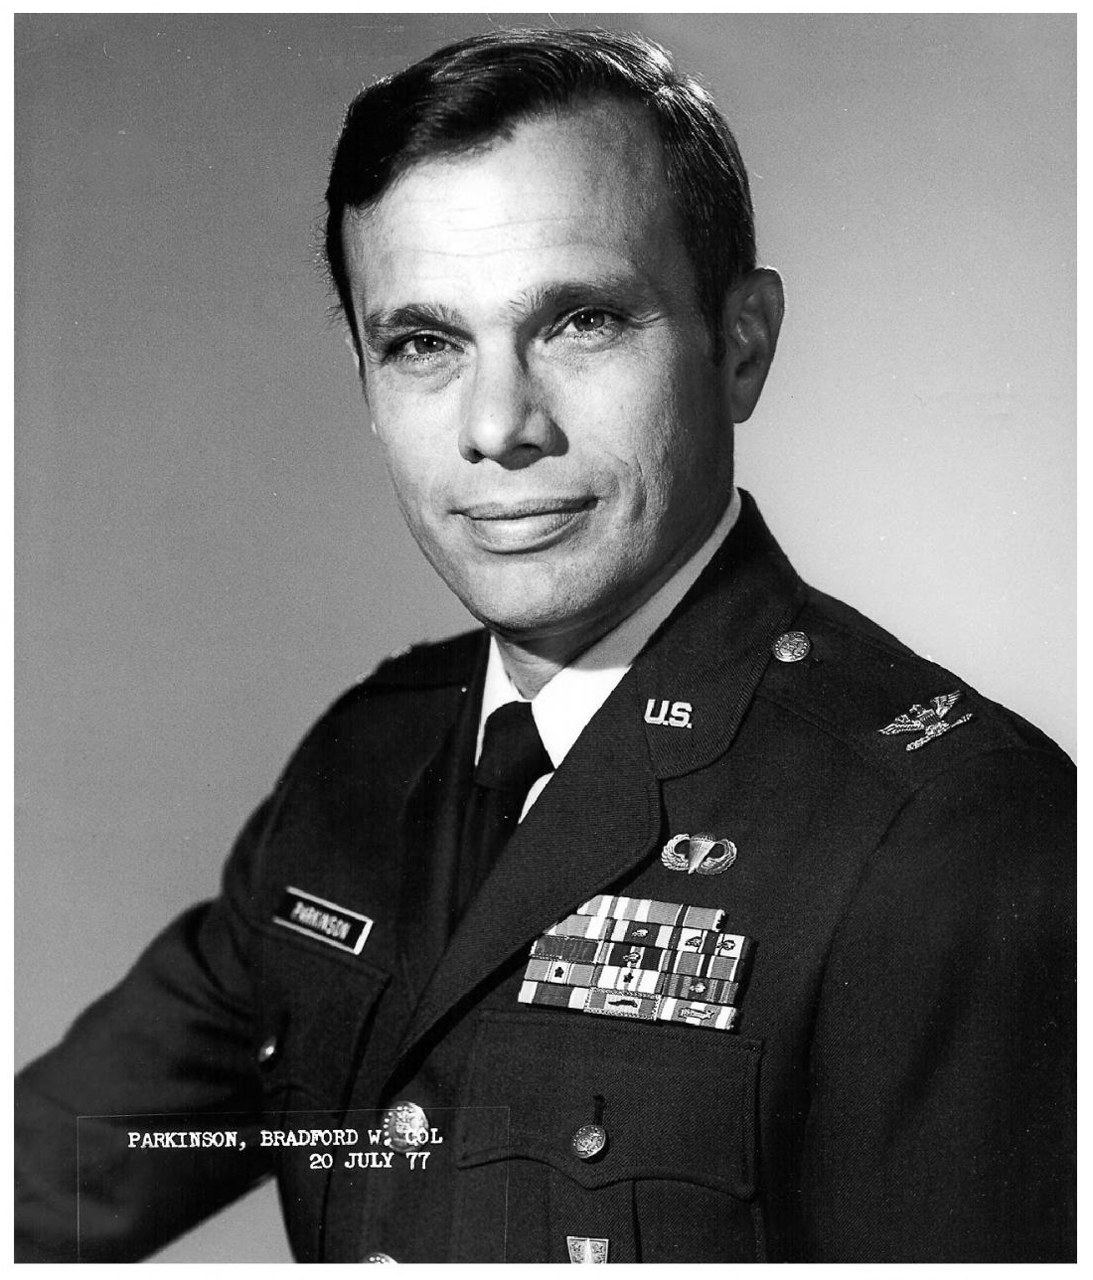
\includegraphics[width=\linewidth]{figs/photos/ch18_parkinson}
\caption{Colonel Bradford Parkinson, chief architect of GPS, in his 1977 official
portrait.\mdccredit{ch18_parkinson}}
\label{fig:ch18_parkinson}
\end{minipage}\hfill
\begin{minipage}[t]{0.6\linewidth}\centering
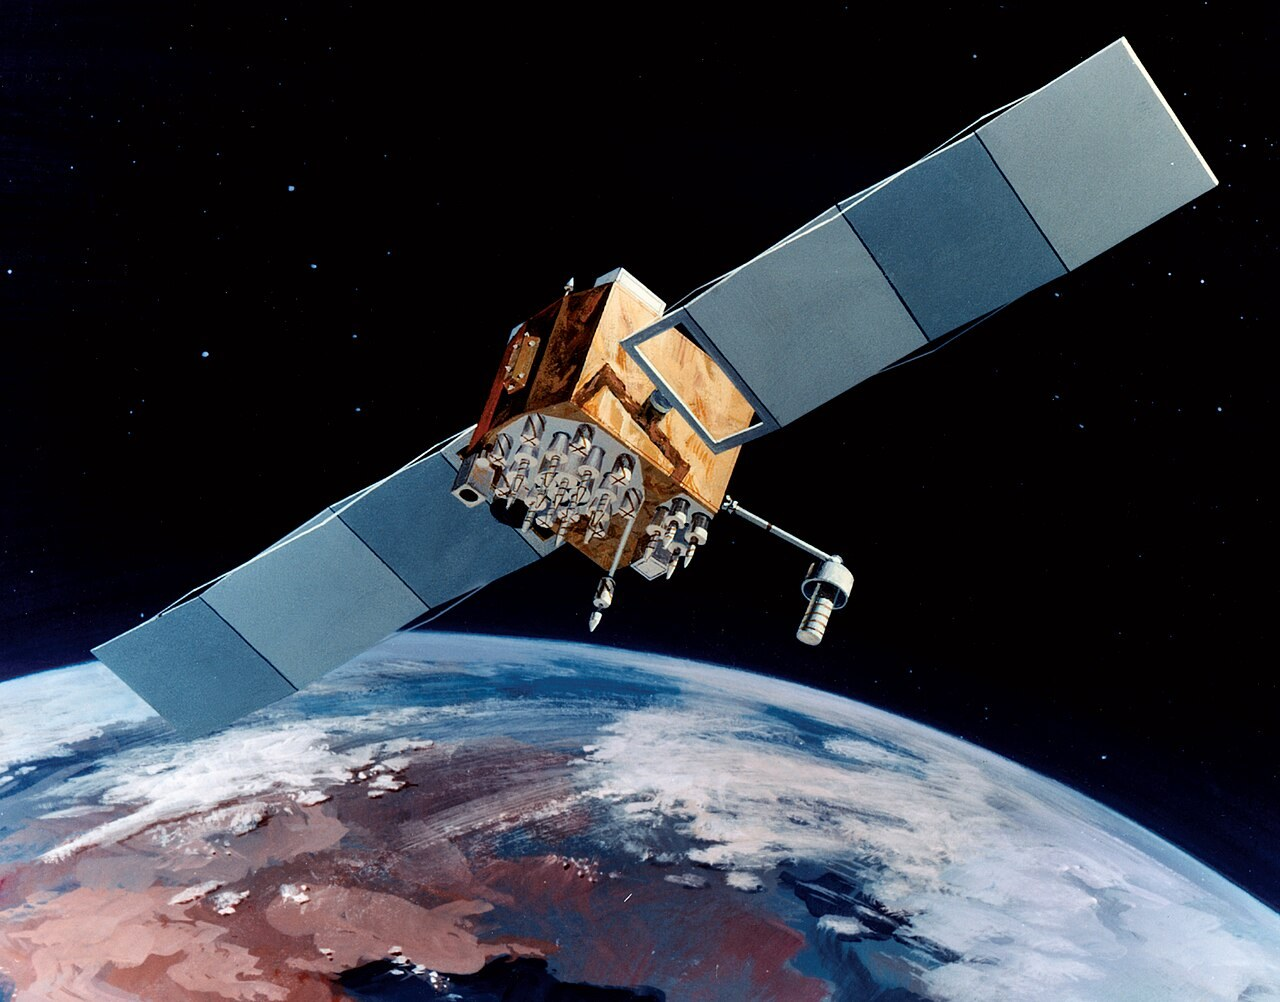
\includegraphics[width=\linewidth]{figs/photos/ch18_gps_iif}
\caption{A GPS Block IIF satellite in orbit (US Air Force artwork). The helix array on the
Earth-facing panel radiates the L-band navigation signals; the satellite carries atomic clocks
and circles the Earth twice a day at 20\,200\,km.\mdccredit{ch18_gps_iif}}
\label{fig:ch18_gps_iif}
\end{minipage}
\end{figure}

\begin{analogy}[Thunder and lightning, run backwards]
You know the trick: count the seconds between the flash and the thunder, and every three seconds
means about a kilometre. GPS is the same trick with the speed of light instead of sound, and
with the satellite telling you exactly when the ``flash'' happened. The catch is the clock.
Light covers 30\,cm in a nanosecond, so a receiver clock that is wrong by a single microsecond
puts you 300\,m off. No pocket device carries an atomic clock---so GPS turns the problem around and
lets the receiver \emph{solve} for its own clock error, using one extra satellite.
\end{analogy}

\begin{history}[From Sputnik's beeps to the Labor Day meeting]
Days after the launch of Sputnik~1 in October 1957, William Guier and George Weiffenbach of
the Johns Hopkins Applied Physics Laboratory found that they could determine the satellite's
orbit from the Doppler shift of its 20\,MHz beacon received at a single known site. Their
colleague Frank McClure turned the problem around: if the orbit were known, the Doppler
curve would locate the receiver. The result was \emph{Transit}, the Navy Navigation Satellite
System (Figures~\ref{fig:ch18_transit_sat} and~\ref{fig:ch18_transit_rx}), developed to fix the positions of ballistic-missile
submarines and operational from 1964. Transit gave a two-dimensional fix good to a few hundred
metres, but only when one of its handful of low satellites passed overhead, sometimes hours apart.
Meanwhile the Naval Research Laboratory's \emph{Timation} programme, led by Roger Easton, flew
precise clocks in orbit, and the Air Force's Project~621B studied pseudo-noise ranging signals.

In 1973 Colonel Bradford Parkinson (Figure~\ref{fig:ch18_parkinson}), newly in charge of the Air
Force's navigation programme, gathered a small group of officers and engineers in the Pentagon over
the Labor Day weekend and merged the competing ideas into one design: satellites in medium Earth
orbit carrying atomic clocks (from Timation), spread-spectrum ranging signals (from 621B), and a
receiver that solves for its clock offset along with its position. The Defense Systems
Acquisition Review Council approved the programme, NAVSTAR GPS, in December 1973. The first
Block~I satellite was launched on 22 February 1978. Full operational capability was declared
in 1995. Its descendants, such as the Block IIF satellite of Figure~\ref{fig:ch18_gps_iif}, still
follow Parkinson's design.
\end{history}

\mdcfig{ch18_trilat_concept}{Ranging with clocks, in two dimensions. (a) With a perfect clock, the
range circles around three satellites meet at a single point: you. (b) A receiver clock that runs
fast makes every measured range too long by the same amount; the circles no longer meet but
enclose a small ``triangle of doubt''. Shrinking every radius by one common amount until they meet
again is exactly what solving for the clock bias $b$ does.}

\subsection{The pseudorange equation}

Let satellite $k$ be at position $\vect s_k$ (known from its broadcast \emph{ephemeris}) when it
transmits at time $t_k$ by its clock. The signal arrives at the user at time $t_u$ by the
user's clock. The \term{pseudorange} is the measured transit time times the speed of light,
\begin{equation}
\rho_k=c\,(t_u-t_k)=\|\vect s_k-\vect u\|+b+c\,\delta t_{\text{sat},k}^{\text{err}}+I_k+T_k+\varepsilon_k,
\label{eq:ch18:pseudorange}
\end{equation}
where $\vect u$ is the user's position, $b=c\,\delta t_u$ is the user clock bias in metres,
and the remaining terms are the residual satellite clock error, the ionospheric and
tropospheric delays and everything else (multipath, receiver noise). It is called a
\emph{pseudo}range because it is the true range plus junk---mostly the receiver's clock error.
After the corrections of Section~\ref{sec:ch18:errors} are applied, the model is
\begin{equation}
\rho_k=\|\vect s_k-\vect u\|+b+\varepsilon_k,\qquad k=1,\dots,K.
\label{eq:ch18:prmodel}
\end{equation}
There are four unknowns: $u_x,u_y,u_z,b$. Hence the famous requirement of four satellites.
Geometrically (Figures~\ref{fig:ch18_trilat_concept} and~\ref{fig:ch18_trilateration}), each true
range defines a sphere around a satellite, and the user is where the spheres intersect; the clock
bias inflates every sphere by the same unknown amount, and the fourth satellite fixes it. A
receiver with a perfect clock would need three, and one that knows its height (a ship, say) can use
the Earth's surface as one of the spheres.

\begin{figure}[htbp]\centering
\begin{tikzpicture}
% ---- (a) overall geometry
\begin{scope}
\fill[navy!6] (-3.0,-0.45) rectangle (3.0,0);
\draw[navy!60,thick] (-3.0,0) -- (3.0,0);
\node[font=\sffamily\tiny,text=navy!70] at (2.2,-0.25) {Earth's surface};
\coordinate (U) at (0,0);
\foreach \a/\n in {140/1,95/2,60/3,25/4}{
  \coordinate (S\n) at (\a:3.6);
  \draw[accent!70,dashed] (U) -- (S\n);
  \fill[navy] (S\n) circle (2.2pt);
  \node[font=\sffamily\scriptsize,anchor=south] at ([yshift=2pt]S\n) {sat.~\n};
}
\fill[green!50!black] (U) circle (2.4pt);
\node[font=\sffamily\scriptsize,text=green!40!black,anchor=north] at (0,-0.05) {user};
\draw[navy!70] (-0.55,-0.55) rectangle (0.55,0.55);
\node[font=\sffamily\scriptsize] at (0,-0.85) {(a) four satellites in view};
\end{scope}
% ---- (b) zoom on the user
\begin{scope}[xshift=7.2cm,yshift=1.4cm]
\draw[navy!70] (-2.3,-1.9) rectangle (2.3,2.0);
\clip (-2.3,-2.0) rectangle (2.3,2.0);
\foreach \a/\n in {140/1,95/2,60/3,25/4}{
  % true range: line through the user, perpendicular to the satellite direction
  \draw[navy!60] ($(0,0)+(\a+90:1.7)$) -- ($(0,0)+(\a-90:1.7)$);
  % pseudorange: the same line pushed 0.75 away from the satellite
  \draw[accent,thick] ($(\a+180:0.75)+(\a+90:1.7)$) -- ($(\a+180:0.75)+(\a-90:1.7)$);
  \draw[-{Stealth[length=1.5mm]},navy!50] (0,0) -- (\a:0.9) node[font=\tiny,text=navy,fill=white,inner sep=1pt] {\n};
}
\fill[green!50!black] (0,0) circle (2.4pt);
\end{scope}
\node[font=\sffamily\scriptsize] at (7.2,-0.85) {(b) close to the user};
\node[font=\sffamily\scriptsize,text=navy!70,anchor=west] at (9.6,2.4) {true ranges $r_k$:};
\node[font=\sffamily\scriptsize,text=navy!70,anchor=west] at (9.6,2.05) {meet at the user};
\node[font=\sffamily\scriptsize,text=accent,anchor=west] at (9.6,1.3) {pseudoranges $\rho_k$:};
\node[font=\sffamily\scriptsize,text=accent,anchor=west] at (9.6,0.95) {all longer by $b$,};
\node[font=\sffamily\scriptsize,text=accent,anchor=west] at (9.6,0.6) {no common point};
\end{tikzpicture}
\caption{The geometry of a GNSS fix (not to scale). (a) Four satellites in view; the arrows in (b)
point towards them. (b) Close to the user, each range sphere is nearly a plane perpendicular to
the satellite direction. The true ranges $r_k$ (thin lines) all pass through the user. The
measured pseudoranges (thick lines) are all longer by the same clock bias $b$, so they do not meet
at a point; the receiver finds the position and the single bias that make them consistent. In
reality the satellites are about 20\,000\,km up and the ranges are spheres.}
\label{fig:ch18_trilateration}
\end{figure}

\subsection{Solving for position and time}

Equation~\eqref{eq:ch18:prmodel} is non-linear in $\vect u$, but it is smooth, and the standard
solution is the engineer's favourite trick: guess, straighten the problem out around the guess,
solve the straight version, and repeat. Linearise about a guess $\vect x_0=(\vect u_0,b_0)$. Let
$r_{k,0}=\|\vect s_k-\vect u_0\|$ and let $\vect e_k=(\vect s_k-\vect u_0)/r_{k,0}$ be the unit
vector from the guess to satellite $k$. To first order,
\begin{equation}
\rho_k\approx r_{k,0}-\vect e_k^{\mathsf T}(\vect u-\vect u_0)+b.
\end{equation}
Stacking the $K$ measurements, with $\Delta\rho_k=\rho_k-r_{k,0}-b_0$ and
$\Delta\vect x=\vect x-\vect x_0$,
\begin{equation}
\Delta\boldsymbol\rho=\vect G\,\Delta\vect x+\boldsymbol\varepsilon,\qquad
\vect G=\begin{bmatrix}-\vect e_1^{\mathsf T}&1\\-\vect e_2^{\mathsf T}&1\\\vdots&\vdots\\-\vect e_K^{\mathsf T}&1\end{bmatrix}.
\label{eq:ch18:linear}
\end{equation}
With $K\ge4$, the least-squares solution is
\begin{equation}
\Delta\hat{\vect x}=(\vect G^{\mathsf T}\vect G)^{-1}\vect G^{\mathsf T}\Delta\boldsymbol\rho,
\label{eq:ch18:ls}
\end{equation}
and the receiver updates $\vect x_0\leftarrow\vect x_0+\Delta\hat{\vect x}$ and repeats. This is
the Gauss--Newton method. It converges in a handful of iterations even from the centre of the
Earth, because the satellites are far away and the problem is only mildly non-linear. When the
measurements have different accuracies (low-elevation satellites are noisier), a weighted
least-squares solution with $\vect W=\operatorname{diag}(1/\sigma_k^2)$ is used, and in a moving
receiver a Kalman filter (Chapter~\ref{ch:sync}) replaces the snapshot solution, carrying the
position, velocity and clock states from one epoch to the next.

\begin{worked}[A position fix from four satellites]
A receiver in Ottawa (latitude $45.4215^\circ$\,N, longitude $75.6972^\circ$\,W, height 70\,m;
ECEF $\vect u=(1107.854,\,-4345.395,\,4520.400)$\,km) sees four satellites whose ECEF
positions, rounded to the kilometre, are
\begin{center}\small
\begin{tabular}{@{}c r r r r r r@{}}
\toprule
Sat. & $x$ (km) & $y$ (km) & $z$ (km) & az. & el. & $\rho_k$ (m)\\
\midrule
1 & 18\,788 & $-18\,772$ & $-98$ & 140$^\circ$ & 24$^\circ$ & 23\,366\,841.1\\
2 & $-20\,202$ & $-13\,309$ & 10\,963 & 275$^\circ$ & 17$^\circ$ & 24\,084\,232.6\\
3 & 16\,313 & $-9\,282$ & 18\,793 & 74$^\circ$ & 49$^\circ$ & 21\,515\,671.2\\
4 & 9\,331 & $-16\,171$ & 18\,890 & 85$^\circ$ & 76$^\circ$ & 20\,430\,773.1\\
\bottomrule
\end{tabular}
\end{center}
The pseudoranges include a receiver clock bias of 85\,000\,m (a clock error of 283.5\,$\mu$s,
typical of a receiver that has just switched on). Start the iteration~\eqref{eq:ch18:ls} at the
Earth's centre with $b_0=0$. The distance from the true position after each iteration is:
\begin{center}\small
\begin{tabular}{@{}c c c c c c@{}}
\toprule
Iteration & 0 & 1 & 2 & 3 & 4\\
\midrule
Position error & 6367\,km & 1448\,km & 65.3\,km & 133\,m & 2\,cm\\
Clock bias estimate & 0 & 1519\,km & 148.9\,km & 85.134\,km & 85.000\,km\\
\bottomrule
\end{tabular}
\end{center}
Convergence is quadratic once the guess is close: the error falls from 65\,km to 133\,m to
2\,cm, and the 2\,cm that remains is only the rounding of the tabulated pseudoranges to
0.1\,m. With noise-free pseudoranges the answer is exact. With noisy ones the answer inherits the
noise, amplified by the geometry: for this set of satellites $\text{PDOP}=4.1$, so a 1\,m
pseudorange error per satellite gives about 4\,m of position error. The calculation is in
\lab{spread.solve\_position} and in the lab.
\end{worked}

\subsection{Dilution of precision}

Suppose you want to pin down your position by asking friends how far away they are. If your
friends are standing in a tight cluster to the north, their answers barely help you distinguish
``a bit further east'' from ``a bit further west''; if they stand all around you, every direction
is pinned. Satellites are the same, and \term{dilution of precision} (DOP) is the number that
measures it. Figure~\ref{fig:ch18_dop_concept} shows the idea with two range measurements, each
uncertain by $\pm\sigma$: crossing at a wide angle they pin you in a small diamond; at a narrow
angle the diamond is long and thin.

\mdcfig{ch18_dop_concept}{Why geometry matters. Each band is one range measurement with its
uncertainty. (a) Two satellites in very different directions: the bands cross at a right angle and
the possible positions form a small diamond. (b) Two satellites in nearly the same direction: the
same measurement errors leave a long, thin diamond. DOP is the factor by which geometry stretches
the range error into a position error.}

If the pseudorange errors are independent with equal variance $\sigma_{\text{UERE}}^2$ (the
\emph{user equivalent range error}), the covariance of the least-squares
solution~\eqref{eq:ch18:ls} is
\begin{equation}
\operatorname{cov}(\Delta\hat{\vect x})=\sigma_{\text{UERE}}^2\,(\vect G^{\mathsf T}\vect G)^{-1}=\sigma_{\text{UERE}}^2\,\vect Q.
\end{equation}
The matrix $\vect Q$ depends only on the geometry. Expressed in local east--north--up
coordinates, its diagonal elements define the dilution of precision:
\begin{equation}
\begin{gathered}
\text{HDOP}=\sqrt{Q_{EE}+Q_{NN}},\qquad\text{VDOP}=\sqrt{Q_{UU}},\\
\text{PDOP}=\sqrt{Q_{EE}+Q_{NN}+Q_{UU}},\qquad\text{TDOP}=\sqrt{Q_{bb}},
\end{gathered}
\end{equation}
and $\text{GDOP}=\sqrt{\operatorname{tr}\vect Q}$. The position error is roughly
\begin{equation}
\sigma_{\text{position}}\approx\text{PDOP}\times\sigma_{\text{UERE}}.
\end{equation}
Good geometry has satellites spread around the sky with at least one high and several low;
bad geometry has them bunched together, so that the unit vectors $\vect e_k$ are nearly
parallel and $\vect G^{\mathsf T}\vect G$ is nearly singular (Figure~\ref{fig:ch18_position}).
Vertical accuracy is always worse than horizontal (VDOP $>$ HDOP), because satellites below
the horizon cannot be seen: all the $\vect e_k$ have positive up-components, so height and
clock bias are partially confounded. In an open-sky location with today's multi-GNSS
constellations, a receiver tracks 30 or more satellites and PDOP is often near 1; in an urban
canyon, with only a slice of sky visible, DOPs of 5--20 are common. Because the satellites move,
the geometry---and the DOP---changes through the day (Figure~\ref{fig:ch18_constellation}).

\mdcfig{ch18_position}{Geometry matters. (a) Satellites spread over the sky, one near the
zenith: PDOP 1.9. (b) Six satellites bunched in the north-east: PDOP 12. (c) Horizontal fixes
from 400 noisy measurement sets ($\sigma_{\text{UERE}}=3$\,m) with each geometry; the poor
geometry stretches the error cloud along the direction the satellites cannot constrain.}

\begin{tryit}[Friends in a cluster]
Open Lab~25's \emph{Position fix and DOP} (Figure~\ref{fig:ch18_lab_e8}). With \emph{Sky} set to ``Good: spread over the sky'',
note the PDOP readout and the size of the 400-fix cloud. Switch to ``Poor: clustered'' and then to
``Urban canyon (high only)'' without touching \emph{Pseudorange error $\sigma$}: the cloud stretches
by the PDOP ratio. Drag \emph{Receiver clock error} anywhere you like---the solver recovers it every
time, and the convergence plot shows Gauss--Newton arriving in four or five steps.
\end{tryit}

\mdcfig{ch18_constellation}{(a) Sky tracks of the satellites of an idealised 24-satellite GPS
constellation over six hours as seen from 45$^\circ$\,N (dots mark the end of each track).
(b) The number of satellites above 10$^\circ$ elevation and the PDOP and HDOP over a day. The
real GPS constellation has about 31 satellites in unevenly spaced slots, and a multi-GNSS
receiver sees three to four times as many satellites, which makes DOP spikes like these rare.}

\subsection{Time, coordinates and relativity}

The satellites' positions are given in an Earth-centred, Earth-fixed (ECEF) frame, WGS-84 for
GPS, and the receiver converts its ECEF answer to latitude, longitude and height above the
WGS-84 ellipsoid. Two subtleties arise from the fact that the frame rotates. During the
roughly 70\,ms the signal is in flight, the Earth turns, carrying the receiver up to about
30\,m eastwards. The receiver must therefore rotate each satellite's position by
$\Omega_E\,\tau_k$ about the polar axis (the \emph{Sagnac} or Earth-rotation correction)
before solving. Omitting it produces errors of tens of metres.

\term{GPS time} is a continuous atomic time scale that began at midnight UTC on 6 January
1980. It has no leap seconds, so it differs from UTC by the number of leap seconds inserted
since 1980---18\,s since 2017---a number the navigation message broadcasts. Galileo, BeiDou
and GLONASS keep their own system times, and the offsets between them are broadcast or
estimated as an extra unknown in a multi-constellation fix (one clock unknown per system,
so a multi-GNSS solution needs a satellite for each extra unknown).

\mdcpairany{ch18_relativity}{Einstein in the sky (computed from the formulas in the text).
(a) Weaker gravity makes a GPS satellite clock gain about 45.7\,$\mu$s a day; its orbital speed
makes it lose about 7.2. (b) Left uncorrected, the net 38\,$\mu$s/day would grow into a range error
of about 11.5\,km in a single day.}{ch18_hmaser}{A passive hydrogen maser, the master clock of a
Galileo satellite. Clocks like this, drifting by roughly a nanosecond a day, are why the
relativistic offsets must be---and can be---corrected.}

Satellite clocks also need relativity---and this is not a footnote, it is a daily kilometre-sized
effect (Figure~\ref{fig:ch18_relativity}). A clock in a GPS orbit (radius about 26\,560\,km) sits
higher in the Earth's gravitational potential than one on the ground and so runs \emph{fast},
by the general-relativistic fractional amount
\begin{equation}
\frac{\Delta f}{f}\bigg|_{\text{GR}}=\frac{GM_E}{c^2}\left(\frac1{R_E}-\frac1a\right)\approx5.3\times10^{-10},
\end{equation}
about $+45.7\,\mu$s per day. It also moves at about 3.87\,km/s, so by special relativity it runs
\emph{slow} by $v^2/2c^2\approx8.3\times10^{-11}$, about $-7.2\,\mu$s per day. The net effect is
$+38.4\,\mu$s per day, or $4.45\times10^{-10}$. Uncorrected, it would accumulate a range error
of $38.4\,\mu\text{s}\times c\approx11.5$\,km per day. GPS corrects most of it in hardware:
the satellite clocks' nominal 10.23\,MHz frequency is set to 10.229\,999\,995\,43\,MHz before
launch, so that it appears as exactly 10.23\,MHz on the ground---a correction that only makes
sense because the onboard clocks (Figure~\ref{fig:ch18_hmaser}) are stable enough to show it. A remaining periodic term,
caused by the small eccentricity of the orbit, is corrected by the receiver as
$\Delta t_r=F\,e\sqrt{a}\,\sin E_k$, with $F=-4.442807633\times10^{-10}$\,s/m$^{1/2}$ (IS-GPS-200);
for $e=0.01$ its amplitude is about 23\,ns, or 7\,m. GPS is a working, everyday confirmation of
both of Einstein's theories.

\mdcphoto[0.5]{ch18_etrex}{A handheld GPS and GLONASS receiver. The screen shows the receiver's own
sky plot and a bar of $C/N_0$ for each satellite tracked---the same quantities this section
computes. Devices like this became affordable consumer products after Selective Availability was
switched off in 2000.}

\begin{history}[KAL007, Selective Availability and the civilian GPS]
GPS was built as a military system, with a coarse civil signal as a by-product. On 1~September
1983 Korean Air Lines flight 007, which had strayed into Soviet airspace through a navigation
error, was shot down, killing all 269 people aboard. Two weeks later the Reagan
administration announced that GPS would be made available for civil aviation once complete.
Civil users were, however, deliberately limited by \emph{Selective Availability} (SA), a
classified dithering of the satellite clocks and ephemerides that degraded the civil
horizontal accuracy to about 100\,m (95\%). Civil engineers responded with differential GPS
(Section~\ref{sec:ch18:augmentation}), which removed SA's errors almost completely and made
it largely pointless. At midnight on 1--2 May 2000, by a decision of President Clinton, SA
was set to zero; overnight the accuracy of every civil receiver improved about tenfold, to
roughly 10\,m, and the consumer GPS industry took off (Figure~\ref{fig:ch18_etrex}). In 2007 the
US government announced that the GPS III satellites would be built without the SA capability at
all.
\end{history}

%======================================================================
\section{GNSS signals}
\label{sec:ch18:signals}
%======================================================================

What exactly does a GPS satellite shout? Every frequency, every code chip and every data bit
it sends is locked to one atomic oscillator, and the design choices made in the 1970s---a
1.023\,Mchip/s code, a 50\,b/s message---still shape every receiver on Earth.

\subsection{GPS L1 C/A: the original civil signal}
\label{sec:ch18:gpsca}

Every frequency in a GPS satellite is derived from one atomic oscillator at
$f_0=10.23$\,MHz. The L1 carrier is $154f_0=1575.42$\,MHz and L2 is $120f_0=1227.60$\,MHz. The
civil \term{C/A code} (coarse/acquisition) runs at $f_0/10=1.023$\,Mchip/s, so one chip lasts
977.5\,ns, or 293\,m of range. Each satellite has its own 1023-chip Gold code, repeating every
millisecond. The code is generated by two 10-stage LFSRs (Figure~\ref{fig:ch18_cagen}),
\begin{equation}
G_1:\;1+x^3+x^{10},\qquad G_2:\;1+x^2+x^3+x^6+x^8+x^9+x^{10},
\end{equation}
both started at all ones at each code epoch. The C/A chip is $G_1\oplus G_2'$, where $G_2'$ is
the modulo-2 sum of two selected stages of $G_2$ (the \emph{phase selector}), which is
equivalent to a delayed copy of the $G_2$ sequence. Each satellite (each PRN number) has its
own pair of taps; PRN~1 uses stages 2 and 6, PRN~2 stages 3 and 7, and so on (IS-GPS-200, Table
3-Ia). The first ten chips of PRN~1 are \texttt{1100100000}, which IS-GPS-200 lists in octal as
1440 as a check for implementers. The 32 codes have periodic cross-correlations taking only
the values $-1$, $-65$ and $63$ (Figure~\ref{fig:ch18_codes}).

\begin{figure}[htbp]\centering
\begin{tikzpicture}[cell/.style={draw=navy,fill=navy!6,minimum size=0.48cm,font=\sffamily\tiny,inner sep=0pt},
  xo/.style={draw=accent,circle,thick,minimum size=0.36cm,inner sep=0pt,font=\scriptsize},
  arr/.style={-{Stealth[length=1.6mm]},navy}]
\foreach \i in {1,...,10}{\node[cell] (a\i) at (0.55*\i,1.6) {\i}; \node[cell] (b\i) at (0.55*\i,0) {\i};}
\node[font=\sffamily\scriptsize,anchor=east] at (0.15,1.6) {$G_1$};
\node[font=\sffamily\scriptsize,anchor=east] at (0.15,0) {$G_2$};
% G1 feedback 3,10
\node[xo] (fa) at (2.2,2.35) {$+$};
\draw[navy] (a3.north) |- (fa.west); \draw[navy] (a10.north) |- (fa.east);
\draw[arr] (fa.north) -- ++(0,0.2) -| ([xshift=-0.35cm]a1.west) -- (a1.west);
% G2 feedback 2,3,6,8,9,10
\node[xo] (fb) at (3.3,-0.85) {$+$};
\foreach \j in {2,3,6,8,9,10}{\draw[navy] (b\j.south) -- ++(0,-0.25) -- ++(0,0);}
\draw[navy] ([yshift=-0.25cm]b2.south) -- ([yshift=-0.25cm]b10.south);
\draw[navy] (fb.north) -- ++(0,0.1);
\draw[arr] (fb.south) -- ++(0,-0.25) -| ([xshift=-0.35cm]b1.west) -- (b1.west);
% phase selector
\node[xo] (ps) at (3.3,0.8) {$+$};
\draw[green!50!black] (b2.north) |- (ps.west); \draw[green!50!black] (b6.north) |- (ps.east);
\node[font=\sffamily\tiny,text=green!40!black,align=center] at (4.9,0.8) {phase selector\\(PRN 1: 2, 6)};
% output
\node[xo] (out) at (7.0,0.8) {$+$};
\draw[navy] (a10.east) -| (out.north);
\draw[navy] (ps.south) |- (3.3,0.45) -| (out.south);
\draw[arr] (out.east) -- ++(0.6,0) node[right,font=\sffamily\scriptsize,align=left] {C/A code\\1.023 Mchip/s};
\node[font=\sffamily\scriptsize,text=navy!70] at (8.05,-0.5) {clock: 1.023 MHz};
\end{tikzpicture}
\caption{The GPS C/A code generator. Two 10-stage shift registers with fixed feedback produce
the $G_1$ and $G_2$ m-sequences; the C/A chip is $G_1$'s output XORed with the sum of two
satellite-specific stages of $G_2$, which selects one member of a Gold family. Both registers
reset to all ones every 1023 chips (1\,ms). \lab{commlib.spread.gps\_ca\_code} implements it
in a dozen lines.}
\label{fig:ch18_cagen}
\end{figure}

The C/A code is modulo-2 added to the 50\,b/s \term{navigation message}
(Figure~\ref{fig:ch18_navmsg}). Each data bit spans exactly 20 code periods, and bit edges coincide
with code epochs. The message is organised in 1500-bit frames of five 300-bit subframes, each
lasting 6\,s and made of ten 30-bit words with (32,26) Hamming-type parity. Each subframe begins
with a telemetry word containing an 8-bit preamble (\texttt{10001011}) and a handover word
containing the time of week. Subframe~1 carries the satellite clock correction and health;
subframes 2 and 3 the satellite's own precise orbit, the \term{ephemeris}, as Keplerian elements
with perturbation terms, valid for about four hours; subframes 4 and 5 rotate through 25 pages of
\term{almanac} (coarse orbits of all satellites), ionospheric model coefficients and UTC
parameters, so the full message takes 12.5 minutes. A receiver needs about 18--30\,s of clean
signal to collect a satellite's ephemeris, which is why an unaided cold start takes that long and
why assisted GNSS (Section~\ref{sec:ch18:acq}) delivers the ephemeris over the cellular network
instead.

\begin{figure}[htbp]\centering
\begin{tikzpicture}[
  sf/.style={draw=navy,thick,minimum height=0.75cm,minimum width=2.25cm,align=center,font=\sffamily\scriptsize},
  wd/.style={draw=navy!70,minimum height=0.55cm,minimum width=1.08cm,align=center,font=\sffamily\tiny}]
\node[sf,fill=accent!12] (s1) at (0,0) {Subframe 1\\clock, health};
\node[sf,fill=green!12] (s2) at (2.3,0) {Subframe 2\\ephemeris I};
\node[sf,fill=green!12] (s3) at (4.6,0) {Subframe 3\\ephemeris II};
\node[sf,fill=orange!12] (s4) at (6.9,0) {Subframe 4\\almanac, iono, UTC};
\node[sf,fill=orange!12] (s5) at (9.2,0) {Subframe 5\\almanac};
\node[font=\sffamily\scriptsize,text=navy] at (4.6,0.75) {one frame: 1500 bits, 30\,s at 50\,b/s};
\draw[navy!50,dashed] (s2.south west) -- (-1.1,-1.0);
\draw[navy!50,dashed] (s2.south east) -- (10.3,-1.0);
\node[wd,fill=accent!10] (w1) at (-0.55,-1.3) {TLM\\preamble};
\node[wd,fill=accent!10] (w2) at (0.55,-1.3) {HOW\\time of week};
\foreach \k in {3,...,10}{\node[wd,fill=navy!5] at (0.55+1.1*\k-2.2,-1.3) {word \k};}
\node[font=\sffamily\scriptsize,text=navy] at (4.6,-1.95) {one subframe: 10 words of 30 bits (24 data + 6 parity) = 6\,s};
\node[font=\sffamily\scriptsize,text=green!40!black] at (4.6,-2.4) {one bit = 20\,ms = 20 repetitions of the 1023-chip C/A code};
\end{tikzpicture}
\caption{The legacy GPS navigation message. Five 6-second subframes make a 30-second frame;
each subframe starts with a telemetry word (with the preamble \texttt{10001011}) and a handover word
carrying the time of week. Subframes 1--3 repeat every frame, so a receiver can read a satellite's
clock and ephemeris in about 18--30\,s; subframes 4 and 5 cycle through 25 pages, so the whole
almanac takes 12.5 minutes.}
\label{fig:ch18_navmsg}
\end{figure}

The signal is BPSK: $s(t)=\sqrt{2P}\,c(t)\,d(t)\cos(2\pi f_{L1}t)$, in quadrature with the
military P(Y) code. Its spectrum is the $\sinc^2$ of BPSK at 1.023\,Mchip/s, with a main lobe
2.046\,MHz wide (Figure~\ref{fig:ch18_gnss_spectra}b), notated BPSK(1) or BPSK-R(1) in the GNSS
literature, the number counting multiples of 1.023\,MHz.

\mdcfig{ch18_gnss_spectra}{(a) Where the GNSS signals live: the upper L band
(1559--1610\,MHz) and the lower L band (1164--1215\,MHz) are allocated to radionavigation
satellite services and protected for aeronautical use, while 1215--1300\,MHz is shared with
radars; widths are approximate main-lobe or allocated bandwidths. (b) Spectra of signals
centred at 1575.42\,MHz: the C/A code's BPSK(1), the military P(Y) code's BPSK(10), the
BOC(1,1) and MBOC civil signals, and the split M code BOC(10,5).}

\subsection{The military code and the modernised signals}

The \emph{precision} code P runs at 10.23\,Mchip/s on both L1 and L2, with a period of one
week. Since 1994 it has been encrypted into the Y code (``anti-spoofing''), with an
encryption sequence of roughly 500\,kchip/s, so only authorised receivers can use it directly.
Its ten-times-wider bandwidth gives ten times sharper correlation, which is why civil
surveyors went to great lengths to exploit P(Y) on L2 without the key, by
\emph{semi-codeless} tracking that correlates the L1 and L2 P(Y) signals with each other.

GPS modernisation, from the early 2000s onwards, added three civil signals and a new military
one, each improving on C/A:
\begin{description}[style=nextline,leftmargin=1.2em,font=\sffamily\bfseries\small\color{navy}]
\item[L2C (1227.60\,MHz).] Two codes time-multiplexed chip by chip at 511.5\,kchip/s each: a
moderate code of 10\,230 chips (20\,ms) carrying data, and a long dataless \emph{pilot} code of
767\,250 chips (1.5\,s). With a pilot, the receiver can integrate coherently for as long as its
oscillator allows and track with a true PLL rather than a Costas loop, gaining about 6\,dB in
tracking threshold. L2C gave civil users a second frequency for ionospheric correction.
\item[L5 (1176.45\,MHz).] In a band protected for aeronautical radionavigation, at
10.23\,Mchip/s with 10\,230-chip codes, a data channel and a pilot channel in quadrature, the
data protected by a convolutional code and short Neuman--Hofman overlay codes that speed up
bit synchronisation. The safety-of-life signal for aviation, and the second frequency of
dual-frequency smartphones.
\item[L1C (1575.42\,MHz).] Designed in cooperation with Europe to be interoperable with Galileo
E1 (and, as it turned out, with China's later BeiDou B1C): 10\,230-chip Weil codes at
1.023\,Mchip/s, 75\% of the power in a pilot, LDPC-coded data, and the multiplexed binary offset
carrier (MBOC) spectrum described next.
\item[M code.] A new encrypted military signal on L1 and L2 using BOC(10,5) modulation, whose
spectrum (Figure~\ref{fig:ch18_gnss_spectra}b) has its energy at $\pm10$\,MHz from the
carrier, away from the civil signals in the centre, so that civil signals can be jammed
locally without jamming M code, and the reverse.
\end{description}

\mdcpairany{ch18_gps_iii}{A GPS Block III satellite (US Air Force artwork). Block III brought the
fourth civil signal, L1C, and higher-power military M code, and was built without the Selective
Availability capability.}{ch18_galileo}{A Galileo Full Operational Capability satellite being
prepared for acoustic testing at ESA's ESTEC centre. Each Galileo satellite carries passive
hydrogen masers and rubidium clocks.}

\subsection{Binary offset carrier modulation}

How do you fit new signals into a band that is already occupied, without stepping on the old
ones? Move their energy to the sides. A \term{binary offset carrier} signal BOC($m,n$) multiplies
the spreading code (chip rate $n\times1.023$\,MHz) by a square-wave subcarrier at
$m\times1.023$\,MHz. The square wave shifts the code spectrum to $\pm m\times1.023$\,MHz, splitting
it into two lobes like a parting crowd.

\Needspace{8\baselineskip}
\begin{deeper}[The BOC spectrum]
For sine-phased BOC with an even number $k=2m/n$ of subcarrier half-periods per chip, the
unit-power PSD is
\begin{equation}
S_{\text{BOC}}(f)=f_c\left[\frac{\sin(\pi f/f_c)\,\tan\!\big(\pi f/(2f_s)\big)}{\pi f}\right]^2,
\end{equation}
with $f_c$ the chip rate and $f_s$ the subcarrier frequency. The $\sin(\pi f/f_c)/(\pi f)$ factor
is the familiar BPSK $\sinc$; the $\tan$ factor is the square-wave subcarrier, which vanishes at
$f=0$ and pushes the energy out to $\pm f_s$.
\end{deeper}

\mdcfig[0.55]{ch18_boc_acf}{The price of a split spectrum (simulated). BOC(1,1) has a correlation
peak about three times steeper than the C/A code's BPSK(1) triangle, which sharpens code tracking,
but it also has negative side peaks of half height at $\pm0.5$\,chip on which a careless loop can
lock.}

Two benefits follow. The split spectrum shares the band with the BPSK signals already there while
overlapping them little. And the signal's RMS bandwidth, its \emph{Gabor bandwidth}, is larger than
that of BPSK at the same chip rate, which sharpens the correlation peak and improves code-tracking
accuracy and multipath resistance for the same receiver bandwidth (Chapter~\ref{ch:sync}: timing
accuracy scales with RMS bandwidth). The cost is a correlation function with side
peaks---BOC(1,1) has negative side peaks of half the main-peak height at $\pm0.5$\,chip---on which
a careless tracking loop can lock (Figure~\ref{fig:ch18_boc_acf}). The interoperable L1C/E1/B1C signals use MBOC, a mixture of
BOC(1,1) with a little BOC(6,1) (1/11 of the power) that adds high-frequency energy for the
receivers wide enough to use it.

\subsection{The other constellations}

GPS is no longer alone in the sky. Four global systems and two regional ones now broadcast
(Table~\ref{tab:ch18:gnss}). Multi-constellation receivers combine them all, which has transformed
availability in cities: a smartphone in the 2020s routinely tracks 30--40 satellites, from
modernised GPS (Figure~\ref{fig:ch18_gps_iii}) and Galileo (Figure~\ref{fig:ch18_galileo}) as well
as the others.

\begin{table}[htbp]\centering\small
\caption{Satellite navigation systems (approximate figures; constellations are still being
replenished and modernised).}
\label{tab:ch18:gnss}
\begin{tabularx}{\linewidth}{@{}>{\raggedright\arraybackslash}p{1.6cm} >{\raggedright\arraybackslash}p{1.1cm} >{\raggedright\arraybackslash}p{3.4cm} >{\raggedright\arraybackslash}X@{}}
\toprule
System & Operator & Orbits & Signals and notes\\
\midrule
GPS & USA & $\sim$31 MEO, 20\,200\,km, 55$^\circ$, 6 planes & L1 C/A, L1C, L2C, L5, P(Y), M; CDMA\\
GLONASS & Russia & $\sim$24 MEO, 19\,100\,km, 64.8$^\circ$, 3 planes & FDMA: G1 $1602+0.5625k$\,MHz, G2 $1246+0.4375k$\,MHz ($k=-7\ldots6$), 511\,kchip/s m-sequence; newer CDMA signals (L3OC)\\
Galileo & EU & $\sim$24--30 MEO, 23\,222\,km, 56$^\circ$, 3 planes & E1 OS (CBOC), E5a/E5b (AltBOC, 1191.795\,MHz), E6 (High Accuracy Service); OSNMA authentication; passive hydrogen masers\\
BeiDou (BDS-3) & China & MEO plus GEO and inclined geosynchronous (IGSO) & B1I, B1C, B2a, B2b, B3I; global service from 2020; regional short-message service\\
QZSS & Japan & IGSO ``quasi-zenith'' plus GEO & GPS-compatible L1, L2C, L5, L1C; L6 centimetre-level augmentation (CLAS)\\
NavIC & India & GEO and IGSO & L5 and S band (2492.028\,MHz); regional\\
\bottomrule
\end{tabularx}
\end{table}

GLONASS is the odd one out: until recently it used frequency division, giving each satellite
the same m-sequence on a different frequency channel, with antipodal satellites in the same
plane sharing a channel. FDMA is robust against narrowband interference but costs receiver
complexity, since each channel has slightly different group delay through the front-end
filters, a bias that must be calibrated. QZSS places satellites in highly inclined
geosynchronous orbits so that one is always near the zenith over Japan, where tall buildings
hide low satellites.

%======================================================================
\section{The GNSS receiver}
\label{sec:ch18:receiver}
%======================================================================

Now for the machine that does the impossible every second of every day: hears thirty signals,
each far below the noise, sorts them out by their codes, and times each one to a few nanoseconds.
Figure~\ref{fig:ch18_gnss_rx} shows the architecture of a modern GNSS receiver. Almost all of
it after the analogue-to-digital converter is software or programmable hardware, and the
reader can build a working one from the figure script and the lab.

\begin{figure}[htbp]\centering
\begin{tikzpicture}[
  blk/.style={draw=navy,fill=navy!6,thick,minimum height=0.8cm,minimum width=1.25cm,align=center,font=\sffamily\scriptsize},
  dsp/.style={blk,fill=green!6,draw=green!50!black},
  sw/.style={blk,fill=accent!6,draw=accent},
  arr/.style={-{Stealth[length=2mm]},thick,navy}]
\node[blk] (ant) {RHCP\\antenna};
\node[blk,right=0.3cm of ant] (lna) {LNA\\NF 1--2\,dB};
\node[blk,right=0.3cm of lna] (flt) {SAW/BAW\\filter};
\node[blk,right=0.3cm of flt] (mix) {Mixer to\\IF or zero-IF};
\node[blk,right=0.3cm of mix] (adc) {ADC 2--8 bits\\$f_s$ 2--50\,MHz};
\node[blk,below=0.45cm of mix] (tcxo) {TCXO\\synthesiser};
\draw[arr] (ant) -- (lna); \draw[arr] (lna) -- (flt); \draw[arr] (flt) -- (mix); \draw[arr] (mix) -- (adc);
\draw[arr] (tcxo) -- (mix); \draw[arr] (tcxo) -| (adc);
\node[dsp,below=1.6cm of flt,minimum width=2.0cm] (acq) {Acquisition\\FFT code search\\over Doppler};
\node[dsp,right=0.5cm of acq,minimum width=3.2cm,minimum height=1.25cm] (trk) {Tracking channels (one per signal)\\carrier NCO, code NCO, E/P/L correlators\\DLL, Costas PLL / FLL};
\node[sw,right=0.5cm of trk] (nav) {Data: bit/frame\\sync, ephemeris};
\node[sw,below=0.45cm of trk,minimum width=3.2cm] (pvt) {Measurements: pseudorange,\\Doppler, carrier phase, $C/N_0$};
\node[sw,right=0.5cm of pvt] (sol) {PVT solution\\least squares /\\Kalman filter};
\draw[arr] (adc.south) |- ([yshift=0.3cm]acq.north) -- (acq.north);
\draw[arr] (adc.south) |- ([yshift=0.3cm]trk.north) -- (trk.north);
\draw[arr] (acq) -- node[above,font=\tiny]{$\hat f_D,\hat\tau$} (trk);
\draw[arr] (trk) -- (nav); \draw[arr] (trk) -- (pvt); \draw[arr] (pvt) -- (sol); \draw[arr] (nav) -- (sol);
\node[blk,left=0.5cm of pvt,font=\sffamily\scriptsize,fill=white,draw=navy!50,dashed] (aid) {Assistance (A-GNSS):\\time, ephemeris,\\approx.\ position};
\draw[arr,dashed] (aid) -- (acq);
\draw[arr,dashed] (sol.south) -- ++(0,-0.35) -| node[pos=0.25,below,font=\tiny]{aiding (vector tracking)} (trk.south west);
\end{tikzpicture}
\caption{Architecture of a GNSS receiver. The RF front end amplifies, filters, downconverts
and digitises the whole band containing the signals; everything after the ADC is digital.
Acquisition finds each satellite's code phase and Doppler; tracking channels follow them and
produce pseudorange, Doppler and carrier-phase measurements and the navigation data; the
navigation processor computes position, velocity and time (PVT). Assistance data from a
network shortens acquisition and the time to first fix.}
\label{fig:ch18_gnss_rx}
\end{figure}

\subsection{The front end}

The antenna is right-hand circularly polarised, matching the satellites, which rejects
reflections that have flipped to left-hand polarisation on a single bounce. Typical antennas
are ceramic patches with a few dBi of gain toward the zenith and much less toward the
horizon; survey antennas use choke rings to suppress reflections from below
(Figure~\ref{fig:ch18_dgps_ref}). A low-noise amplifier sets the noise figure, often at the
antenna, followed by SAW or BAW filters that reject strong out-of-band signals, notably nearby
cellular transmitters. Because the GNSS signal is far below the noise, the ADC sees essentially
Gaussian noise and needs only a few bits: one-bit sampling costs about 2\,dB of SNR
($10\log_{10}(\pi/2)$), two bits about 0.5\,dB. More bits are used when interference must be
handled, since a strong interferer captures a one-bit quantiser completely. Receivers with an
automatic gain control set the ADC level from the noise, and the AGC level itself is a sensitive
jamming detector.

\mdcfig{ch18_acquisition}{(a) Acquisition search space for a synthetic signal: the
correlation power over code phase and Doppler, from four 1\,ms coherent FFT searches added
non-coherently, for a satellite at 44\,dB-Hz in noise; the single peak stands about 25 times
above the median. (b) Detection probability per cell versus $C/N_0$ for a false-alarm
probability of $10^{-6}$ per cell and 1.5\,dB of straddle losses, for coherent integration
times of 1 and 10\,ms and various numbers of non-coherent sums.}

\subsection{Acquisition: the delay--Doppler search}
\label{sec:ch18:acq}

Before tracking a satellite, the receiver must find it---and it is looking for a needle in a
two-dimensional haystack. It must find two unknowns: the code phase (where in the 1023-chip code
the received signal is) and the Doppler shift. A satellite's line-of-sight velocity relative to a
stationary user reaches roughly $\pm800$\,m/s, which at L1 is about $\pm4$\,kHz; the receiver's
oscillator error and its own motion add more, so a cold search typically covers $\pm5$\,kHz or
more. The receiver correlates the incoming signal with local replicas over a grid of trial code
phases and trial Dopplers, and declares detection when a cell's correlation power exceeds a
threshold (Figure~\ref{fig:ch18_acquisition}a).

The grid spacing is set by the correlation function. In delay, the correlation triangle is
two chips wide, so half-chip steps lose at most about 2.5\,dB: 2046 code cells. In frequency,
a coherent integration of length $T$ attenuates a residual frequency error $\Delta f$ by the
factor $|\sinc(\Delta fT)|$, so bins of about $2/(3T)$ are used: 667\,Hz for $T=1$\,ms (the
classic choice is 500\,Hz), giving about 21 bins for $\pm5$\,kHz. The full search has
roughly $2046\times21\approx43\,000$ cells per satellite.

Three search strategies are used:
\begin{description}[style=nextline,leftmargin=1.2em,font=\sffamily\bfseries\small\color{navy}]
\item[Serial search.] Test one cell at a time with a single correlator: the classic hardware
approach. At 1\,ms per cell, a full search of one satellite takes about 43\,s.
\item[Parallel frequency search.] Correlate at one code phase and take an FFT of the
despread samples to test all Doppler bins at once.
\item[Parallel code-phase search.] Wipe off a trial Doppler, then compute the circular
correlation with the local code for all code phases at once using FFTs:
\begin{equation}
\vect z=\mathrm{IFFT}\big(\mathrm{FFT}(\vect x\,e^{-j2\pi\hat f_Dt})\cdot\mathrm{FFT}(\vect c)^*\big).
\label{eq:ch18:fftacq}
\end{equation}
Because the C/A code is periodic with period 1\,ms, the circular correlation of a 1\,ms block is
exactly the correlation at every lag. One FFT pair per Doppler bin tests all 2046 (or more)
code phases; 21 bins take a few milliseconds of computation. This is how software receivers,
and the lab, do it (\lab{spread.acquire}).
\end{description}
Modern chips go further, with massively parallel correlators---hundreds of thousands of
them---that search many satellites and cells at once in hardware.

\mdcfig[0.98]{ch18_lab_e6}{Lab~25 running its \emph{GPS acquisition} experiment: controls on the
left, the delay--Doppler search grid with PRN~7's peak, a slice through the peak and the detection
curves in the centre, and the explanation and challenges on the right.}

\paragraph{Integration and sensitivity.} At $C/N_0=45$\,dB-Hz one millisecond of coherent
integration gives an SNR of 15\,dB, ample for detection. Indoors, at 25\,dB-Hz, it gives
$-5$\,dB, hopeless. Longer integration is needed, and it runs into three limits. The data bits
flip the sign every 20\,ms at unknown times, so coherent integration on C/A is limited to
20\,ms unless the bits are known (from assistance data, or by using a pilot channel). The
Doppler bin width shrinks as $1/T$, so the number of cells grows. And the receiver
oscillator's phase noise limits coherence to a few hundred milliseconds even with known
data. Beyond the coherent limit, the receiver adds the squared magnitudes of successive
coherent sums (\emph{non-coherent integration}). This works, but incurs a \emph{squaring
loss}: at low SNR, $K$ non-coherent sums gain only about $\sqrt K$ in effective SNR, not $K$.
Figure~\ref{fig:ch18_acquisition}b shows the detection probabilities: 1\,ms coherent
integration needs about 43\,dB-Hz, while one second of 10\,ms coherent sums added
non-coherently reaches about 20\,dB-Hz.

\begin{tryit}[Find a satellite under the noise]
In Lab~25's \emph{GPS acquisition} (Figure~\ref{fig:ch18_lab_e6}), pick ``PRN 21 (38 dB-Hz)'' in \emph{Satellite to search} and
look for its peak on the search grid. Drag \emph{Signal strength change} down to $-10$\,dB (you
have walked indoors): the peak drowns. Raise \emph{Coherent integration} to 10\,ms and
\emph{Non-coherent sums} to 4 and it comes back. Then search for ``PRN 30 (not in view)'' and see
what a false alarm would have to look like.
\end{tryit}

\begin{worked}[Search time and sensitivity]
A smartphone must acquire satellites indoors at 25\,dB-Hz. With 10\,ms coherent integration,
the coherent SNR is $25-20=5$\,dB, and the Doppler bins must be about 67\,Hz wide, so a
$\pm5$\,kHz uncertainty needs 150 bins, and the full grid holds about $2046\times150\approx
3\times10^5$ cells. To reach $P_d=0.9$ at $P_{fa}=10^{-6}$ needs roughly ten non-coherent
sums (Figure~\ref{fig:ch18_acquisition}b), i.e.\ 100\,ms of signal per cell. A single serial
correlator would take $3\times10^4$\,s, about eight hours, per satellite. Two things bring it
down to a few seconds. Massively parallel correlators test every code phase at once
($2046\times$ speed-up). And \emph{assistance} from the cellular network (A-GNSS, in 3GPP's
LTE Positioning Protocol, TS~36.355, and its NR successor) supplies time to within
microseconds to seconds, the approximate position, and the satellites' ephemerides and
predicted Dopplers, shrinking the frequency uncertainty to a few bins and the code
uncertainty to a fraction of the code when fine time is available. Assistance also supplies
the data bits, so that coherent integration can extend past 20\,ms.
\end{worked}

\begin{figure}[htbp]\centering
\begin{tikzpicture}[
  blk/.style={draw=navy,fill=navy!6,thick,minimum height=0.7cm,minimum width=1.2cm,align=center,font=\sffamily\scriptsize},
  mul/.style={draw=navy,circle,thick,minimum size=0.45cm,inner sep=0pt,font=\small},
  arr/.style={-{Stealth[length=1.8mm]},thick,navy}]
\node[blk] (in) {Samples\\$x_n$};
\node[mul,right=0.4cm of in] (mc) {$\times$};
\node[mul,right=1.0cm of mc,yshift=0.9cm] (me) {$\times$};
\node[mul,right=1.0cm of mc] (mp) {$\times$};
\node[mul,right=1.0cm of mc,yshift=-0.9cm] (ml) {$\times$};
\foreach \n/\l in {e/E,p/P,l/L}{
  \node[blk,right=0.35cm of m\n,minimum width=1.0cm] (i\n) {$\sum$ $T$};
  \node[font=\scriptsize,right=0.05cm of i\n] (o\n) {$\l$};
  \draw[arr] (m\n) -- (i\n);
  \draw[arr] (mc.east) -- ++(0.3,0) |- (m\n.west);
}
\draw[arr] (in) -- (mc);
\node[blk,right=1.1cm of ip,yshift=0.6cm,fill=green!6,draw=green!50!black] (dll) {DLL discr.\\$\frac{|E|-|L|}{|E|+|L|}$};
\node[blk,right=1.1cm of ip,yshift=-0.75cm,fill=accent!6,draw=accent] (pll) {Costas discr.\\$\arctan\frac{Q_P}{I_P}$};
\draw[arr] (oe) -- (dll); \draw[arr] (ol) -- (dll); \draw[arr] (op.east) -- (pll);
\node[blk,right=0.4cm of dll,fill=green!6,draw=green!50!black] (fd) {Loop\\filter};
\node[blk,right=0.4cm of pll,fill=accent!6,draw=accent] (fp) {Loop\\filter};
\draw[arr] (dll) -- (fd); \draw[arr] (pll) -- (fp);
\node[blk,below=1.15cm of ml,xshift=0.2cm,fill=green!6,draw=green!50!black] (cnco) {Code NCO and\\E/P/L generator};
\node[blk,below=0.55cm of mc,xshift=-0.15cm,fill=accent!6,draw=accent,yshift=-0.95cm] (pnco) {Carrier\\NCO};
\draw[arr,green!50!black] (fd.south) |- ([yshift=-0.3cm]cnco.east) -- (cnco.east);
\draw[arr,accent] (fp.south) |- ([yshift=-0.75cm]pnco.south) -- (pnco.south);
\draw[arr,accent] (pnco) -- (mc);
\draw[arr,accent,dashed] (fp.south) |- ([yshift=0.15cm]cnco.east) node[pos=0.75,above,font=\tiny]{carrier aiding $\times\frac{1}{1540}$};
\draw[arr,green!50!black] (cnco.north) -- ++(0,0.25) -| (ml.south);
\draw[green!50!black,thick] ([xshift=-0.45cm]cnco.north) -- ++(0,1.8) -| ($(mp.south)+(-0.05,0)$);
\draw[green!50!black,thick] ([xshift=-0.65cm]cnco.north) -- ++(0,2.7) -| ($(me.south)+(-0.05,0)$);
\end{tikzpicture}
\caption{A GNSS tracking channel. The carrier NCO wipes off the Doppler; early, prompt and late
code replicas are correlated with the result. The delay-locked loop steers the code NCO to
balance $|E|$ and $|L|$; the Costas phase-locked loop steers the carrier NCO to put all the
prompt energy in $I_P$, where the navigation bits appear. The carrier loop's frequency,
scaled by $1.023/1575.42=1/1540$, aids the code loop, so the DLL need only track the
slow divergence between code and carrier (mostly ionospheric).}
\label{fig:ch18_tracking_loops}
\end{figure}

\subsection{Tracking: delay-locked and phase-locked loops}
\label{sec:ch18:tracking}

Finding a satellite is half the battle; staying locked onto it is the other half. Once acquired,
each satellite is handed to a tracking channel that keeps a local carrier and a local code aligned
with the incoming signal, using the loop ideas of Chapter~\ref{ch:sync}.
Figure~\ref{fig:ch18_tracking_loops} shows the structure. The incoming samples are multiplied by
the local carrier (a numerically controlled oscillator, NCO, at the estimated Doppler) and then by
three versions of the local code: \emph{prompt} (P), aligned with the estimate, and \emph{early}
(E) and \emph{late} (L), shifted by $\pm d/2$ chips. Each product is integrated over 1--20\,ms,
giving the complex correlator outputs $E=I_E+jQ_E$, $P=I_P+jQ_P$ and $L=I_L+jQ_L$.

\mdcfig{ch18_dll}{(a) The C/A correlation triangle with early, prompt and late samples at
$d=1$ chip, and the rounding caused by a $\pm2$\,MHz front end. (b) Early-minus-late
discriminator S-curves for three correlator spacings: narrower spacing has a smaller linear
region. (c) Multipath error envelopes for a reflection of half the direct amplitude, in
phase (solid) and out of phase (dashed): a narrow correlator ($d=0.1$) cuts the worst-case
error from about 75\,m to about 7\,m, and is immune to reflections delayed by more than
about 1.05 chips.}

\begin{analogy}[Balancing on a ridge]
The correlation peak is a sharp ridge, and the code loop keeps the receiver standing on top of
it. The early and late correlators are two feet, one on each slope. If the early foot is higher
than the late one, the peak is ahead---step forward; if lower, step back. When both feet are at the
same height you are exactly on the ridge. The narrower your stance (a smaller spacing $d$), the more
precisely you can stand, but the easier it is to slip off if the ridge moves suddenly.
\end{analogy}

\paragraph{The delay-locked loop.} For a code error $\tau$ (in chips) and an ideal correlation
triangle $R(\tau)=1-|\tau|$, the early and late correlator magnitudes are $R(\tau-d/2)$ and
$R(\tau+d/2)$. Their difference is zero when the prompt is aligned and changes sign with
$\tau$, so it can steer the code NCO. Common \term{delay-locked loop} discriminators are the
early-minus-late envelope $|E|-|L|$, the early-minus-late power $|E|^2-|L|^2$, the
dot product $\re\{(E-L)P^*\}$, and normalised versions that divide by $|E|+|L|$ to remove the
dependence on signal amplitude. Inside its linear region, $|\tau|<d/2$, the normalised
envelope discriminator scaled by $(1-d/2)$ reads the code error directly in chips; its
\emph{S-curve} (Figure~\ref{fig:ch18_dll}b) shows the linear region and the pull-in range of
$\pm(1+d/2)$ chips. The tracking jitter due to thermal noise for a coherent
early-minus-late-power DLL is approximately
\begin{equation}
\sigma_\tau^2\approx\frac{B_Ld}{2\,C/N_0}\left[1+\frac{2}{(2-d)\,T\,C/N_0}\right]\quad\text{chips}^2,
\label{eq:ch18:dlljitter}
\end{equation}
where $B_L$ is the loop noise bandwidth and $T$ the integration time; the bracket is the
squaring loss, negligible at high $C/N_0$. The jitter falls with the square root of the
correlator spacing $d$. This is the \term{narrow correlator} idea (Van Dierendonck, Fenton and
Ford, 1992): with a front end wide enough to keep the correlation peak sharp (8\,MHz or more
for C/A), spacing $d=0.1$ instead of 1 reduces the noise jitter by a factor of about three and,
more importantly, the multipath error by about ten (Figure~\ref{fig:ch18_dll}c).

\mdcfig{ch18_tracking}{Tracking a synthetic GPS signal at 42\,dB-Hz with the loops of
\lab{commlib.spread.track}: acquisition left the frequency 67\,Hz in error. (a) The
FLL-assisted carrier loop pulls in within about 150\,ms. (b) The code error, measured against
the truth, settles to a few hundredths of a chip. (c) Once the PLL locks, the prompt energy
moves into $I_P$, which shows the 50\,b/s navigation bits, while $Q_P$ carries only noise.
(d) The prompt correlator in the complex plane: a rotating cloud before lock, two BPSK
clusters after. The $C/N_0$ is estimated from the prompt-correlator statistics.}

\paragraph{The carrier loop.} The navigation data bits flip the sign of the prompt every
20\,ms, so a standard PLL would lose lock at each transition. GNSS receivers therefore use a
\term{Costas loop} (Chapter~\ref{ch:sync}) with a discriminator such as $\arctan(Q_P/I_P)$,
which is insensitive to the sign of the data. When locked, the prompt energy sits in $I_P$
and the data bits can be read off its sign (Figure~\ref{fig:ch18_tracking}c,d); this is
coherent demodulation. The thermal-noise phase jitter is
\begin{equation}
\sigma_\phi\approx\sqrt{\frac{B_L}{C/N_0}\left(1+\frac{1}{2T\,C/N_0}\right)}\quad\text{rad},
\end{equation}
and a common rule keeps the total jitter, including oscillator phase noise and the loop's
dynamic stress error, below about 15$^\circ$ for the arctangent Costas loop, whose pull-in
range is $\pm90^\circ$. Pilot channels allow a pure PLL with a $\pm180^\circ$ range, a gain of
several decibels in tracking threshold. Because a PLL has a narrow pull-in range,
receivers first close a \emph{frequency-locked loop}, whose discriminator uses the phase
change between successive prompt samples, and hand over to the PLL once the frequency error
is small (Figure~\ref{fig:ch18_tracking}a).

\mdcfig[0.98]{ch18_lab_e7}{Lab~25's \emph{DLL and PLL tracking} running live: the code error
settling towards zero, the Costas loop's phase error pulling in after a burst of cycle slips, the
prompt correlator collapsing onto two BPSK clusters, and the 50\,b/s navigation bits emerging on
$I_P$.}

\begin{worked}[Tracking precision]
Take $C/N_0=45$\,dB-Hz ($31\,600$\,Hz), a carrier-aided DLL with $B_L=1$\,Hz, $T=20$\,ms and
$d=1$. From~\eqref{eq:ch18:dlljitter}, $\sigma_\tau^2=\frac{1}{2\times31\,600}(1+0.003)=1.59\times
10^{-5}$\,chips$^2$, so $\sigma_\tau=0.0040$\,chips, or 1.2\,m. With $d=0.1$ it is
0.0013\,chips, or 0.37\,m.

Now the carrier. A Costas loop with $B_L=15$\,Hz and $T=1$\,ms has
$\sigma_\phi=\sqrt{(15/31\,600)(1+0.016)}=0.022$\,rad, or 1.3$^\circ$. The L1 wavelength is
19.0\,cm, so the carrier phase is measured to $0.022/(2\pi)\times19.0\approx0.7$\,mm. The
carrier phase is about a thousand times more precise than the code. That is why
centimetre-level positioning (Section~\ref{sec:ch18:rtk}) uses carrier phase, and why its
difficulty is not precision but the unknown integer number of whole cycles.

A third-order PLL with $B_L=18$\,Hz has natural frequency $\omega_0=B_L/0.7845=22.9$\,rad/s
and a steady-state error of $\dddot R/\omega_0^3$ under a line-of-sight jerk $\dddot R$. For
a manoeuvre of 10\,$g$/s ($98$\,m/s$^3$) this is $98/12\,000=8$\,mm, or 15$^\circ$ of carrier
phase---the whole jitter budget. High-dynamics receivers therefore widen the loop, or aid it
with an inertial measurement unit.
\end{worked}

\begin{tryit}[Keep the lock]
Lab~25's \emph{DLL and PLL tracking} runs a live tracking channel
(Figure~\ref{fig:ch18_lab_e7}). Start with the defaults and
watch the constellation collapse onto the $I$ axis. Now drag \emph{C/N0} down towards 25\,dB-Hz
until the PLL slips; recover by narrowing \emph{PLL bandwidth}. Then add
\emph{Line-of-sight acceleration} of a few $g$: the narrow loop now loses lock, and you have
found the bandwidth trade-off of the worked example for yourself. Try \emph{Early--late spacing}
0.1 and compare the code jitter.
\end{tryit}

\subsection{From correlators to pseudoranges}

Once a channel is tracking, the receiver decodes the data: it finds the bit edges (the
20\,ms boundaries where the sign of $I_P$ can change), searches for the 8-bit preamble of the
telemetry word, checks parity to confirm the subframe alignment, and reads the time of week
from the handover word. It now knows, for any instant, which chip of which code epoch of
which bit of which subframe is arriving---that is, the satellite's transmit time $t_k$ to a
small fraction of a chip. The pseudorange follows from~\eqref{eq:ch18:pseudorange}. Before the
data are decoded, the code phase alone gives the transmit time modulo 1\,ms (300\,km),
an ambiguity that assistance data or an approximate position can resolve.
Figure~\ref{fig:ch18_time_ladder} shows the nested clock the receiver reads, from six-second
subframes down to fractions of a chip.

\begin{figure}[htbp]\centering
\begin{tikzpicture}[
  st/.style={draw=navy,thick,fill=navy!6,minimum height=0.62cm,align=center,font=\sffamily\scriptsize,anchor=west},
  note/.style={font=\sffamily\scriptsize,anchor=west,text=navy!80}]
\node[st,minimum width=12.0cm] (a) at (0,0) {subframe: 6\,s --- start found from the preamble, time of week from the handover word};
\node[st,minimum width=9.6cm,fill=green!8,draw=green!50!black] (b) at (1.2,-0.8) {data bit: 20\,ms --- found from bit edges on $I_P$};
\node[st,minimum width=7.2cm,fill=orange!10,draw=orange] (c) at (2.4,-1.6) {code period: 1\,ms (300\,km)};
\node[st,minimum width=4.8cm,fill=accent!8,draw=accent] (d) at (3.6,-2.4) {chip: 977.5\,ns (293\,m)};
\node[st,minimum width=2.4cm,fill=purple!8,draw=purple] (e) at (4.8,-3.2) {DLL: $\approx$0.004 chip};
\node[note] at (7.4,-3.2) {$\approx$4\,ns, about 1\,m};
\node[note] at (8.6,-2.4) {count chips within the code};
\node[note] at (9.8,-1.6) {count code periods within the bit};
\end{tikzpicture}
\caption{Reading the satellite's transmit time is like reading a clock with five hands. The
navigation message gives the coarse hands (subframe and bit), the code epochs and chip count give
the finer ones, and the delay-locked loop interpolates within a chip to a few nanoseconds.}
\label{fig:ch18_time_ladder}
\end{figure}

The tracking loops also produce two more measurements. The carrier NCO frequency is the
\emph{Doppler}, the rate of change of range, from which the receiver solves for its
velocity with the same geometry matrix $\vect G$, to a few centimetres per second. The
accumulated carrier NCO phase is the \emph{carrier-phase} measurement, a millimetre-precise
but ambiguous range.

\begin{pitfall}[The cold start and the 30-second wait]
A receiver with no information about time, position or the satellites must search all
codes, all Dopplers and all satellites, then decode 18--30\,s of navigation data per satellite
before it can compute a position. The resulting \emph{time to first fix} of 30\,s to a minute
is acceptable for a car navigator but not for an emergency call. Two practices hide the wait.
A \emph{hot} start uses time, position and ephemerides saved from the last session; ephemerides
stay valid for about four hours. \emph{Assisted} GNSS delivers them from the network, and lets
the phone compute a fix in a few seconds even indoors, which is how emergency services
regulations---the US FCC's E911 rules and the European AML and eCall systems---get
positions from handsets. Long-term orbit prediction, computed in the cloud or on the phone,
extends the validity of saved data to days.
\end{pitfall}

%======================================================================
\section{Errors and augmentation}
\label{sec:ch18:errors}
%======================================================================

A phone in the open says it knows where you are to about five metres. A surveyor's receiver on a
tripod claims one centimetre. Both are listening to the same satellites. The difference is
entirely in how they deal with the errors hiding in~\eqref{eq:ch18:pseudorange}
(Figure~\ref{fig:ch18_accuracy_ladder}).

\mdcfig{ch18_accuracy_ladder}{The accuracy ladder (approximate 95\% horizontal figures; real values
depend on sky view, antenna and conditions). Each rung removes another error source: dual
frequency removes the ionosphere, differential corrections remove the errors shared with a nearby
station, and carrier-phase methods trade the metre-level code for the millimetre-level carrier.}

\subsection{The error budget}

Each term of~\eqref{eq:ch18:pseudorange} contributes to the user equivalent range error.
Table~\ref{tab:ch18:errors} lists typical values for single-frequency and dual-frequency
users. The broadcast clock and ephemeris errors of the modern GPS constellation are small; for
single-frequency users the ionosphere dominates, and for dual-frequency users the local
effects of multipath and receiver noise.

\begin{table}[htbp]\centering\small
\caption{Typical one-sigma pseudorange error budget for a code-based GPS receiver, open sky
(approximate engineering values; real errors vary with solar activity, elevation, antenna and
environment).}
\label{tab:ch18:errors}
\begin{tabularx}{\linewidth}{@{}X c c@{}}
\toprule
Error source & Single-frequency L1 C/A & Dual-frequency (iono-free)\\
\midrule
Satellite clock and ephemeris (broadcast) & 0.5--1\,m & 0.5--1\,m\\
Ionosphere, after broadcast (Klobuchar) model & 2--7\,m & $<0.1$\,m\\
Troposphere, after model & 0.2--0.5\,m & 0.2--0.5\,m\\
Multipath (open sky; urban much larger) & 0.5--1\,m & 0.5--1\,m ($\times$ noise factor)\\
Receiver noise & 0.2--0.5\,m & 0.5--1.5\,m\\
\midrule
UERE (root-sum-square) & roughly 3--7\,m & roughly 1--2\,m\\
Horizontal error (HDOP $\approx1$, 95\%) & roughly 5--10\,m & roughly 2--3\,m\\
\bottomrule
\end{tabularx}
\end{table}

\subsection{The ionosphere and dual-frequency positioning}

The biggest single error for a phone is the sky itself. The ionosphere, a layer of free electrons
from about 60 to 1000\,km altitude, is dispersive: it delays the code (group delay) and advances
the carrier phase by the same amount,
\begin{equation}
I=\frac{40.3\,\text{TEC}}{f^2}\quad\text{m},
\label{eq:ch18:iono}
\end{equation}
where TEC is the total electron content along the path in electrons/m$^2$, usually expressed in
TEC units ($10^{16}$\,m$^{-2}$). One TECU delays L1 by 0.16\,m. Vertical TEC ranges from a few
TECU at night at solar minimum to over 100 TECU in the afternoon near the geomagnetic equator at
solar maximum, and slant paths at low elevation see up to three times the vertical value.
Ionospheric delays of 5--30\,m are common and reach 100\,m in storms. Single-frequency receivers
use the 8-coefficient \emph{Klobuchar} model broadcast in the GPS message, which removes
roughly half of the delay; Galileo broadcasts coefficients for the more accurate NeQuick model.

Because the delay scales as $1/f^2$ (Figure~\ref{fig:ch18_iono}), measurements on two frequencies
remove it---like judging the thickness of a pane of glass from how differently it bends red and
blue light. With $\rho_i=r+I_1f_1^2/f_i^2$, the \term{ionosphere-free combination}
\begin{equation}
\rho_{\text{IF}}=\frac{f_1^2\rho_1-f_2^2\rho_2}{f_1^2-f_2^2}
\label{eq:ch18:iflc}
\end{equation}
cancels the first-order term exactly (higher-order terms are a few centimetres at most). The
price is noise: for L1 and L2, $\rho_{\text{IF}}=2.546\rho_1-1.546\rho_2$, which amplifies
independent noise by $\sqrt{2.546^2+1.546^2}\approx3.0$; for L1 and L5 the factor is
about 2.6. This was the reason the military P code was on two frequencies from the start, and
the reason civil L2C and L5 were added.

\mdcfig[0.55]{ch18_iono}{The ionosphere is dispersive: its delay falls as $1/f^2$, so L2 and L5
are delayed about 1.6--1.8 times as much as L1. That difference is what dual-frequency receivers
measure and remove.}

\begin{worked}[Removing the ionosphere]
A satellite at low elevation sees a slant TEC of 50\,TECU. From~\eqref{eq:ch18:iono} the L1
delay is $40.3\times50\times10^{16}/(1575.42\times10^6)^2=8.12$\,m, and the L2 delay is
$8.12\times(1575.42/1227.60)^2=8.12\times1.647=13.37$\,m. If the true range is $r$, the
measurements (ignoring other errors) are $\rho_1=r+8.12$ and $\rho_2=r+13.37$\,m. Then
\[
\rho_{\text{IF}}=2.546(r+8.12)-1.546(r+13.37)=r+20.67-20.67=r.
\]
The difference $\rho_2-\rho_1=5.25$\,m also measures the TEC directly:
$\text{TEC}=5.25\,f_1^2f_2^2/\big(40.3(f_1^2-f_2^2)\big)$, which is how networks of GNSS
receivers map the ionosphere worldwide. If each pseudorange has 0.3\,m of independent noise,
the iono-free combination has $0.3\times3.0=0.9$\,m: a 20\,m bias traded for a little noise.
\end{worked}

\mdcpairany{ch18_dgps_ref}{A GNSS reference-station antenna on a fixed pillar. Its position is
surveyed once, precisely; ever after, the difference between what it measures and what it should
measure is broadcast as a correction.}{ch18_mcs}{The operations floor of the GPS master control
station at Schriever Space Force Base, Colorado, where the 2nd Space Operations Squadron computes
and uploads the satellites' clock and orbit predictions.}

\begin{inpractice}[Dual-frequency phones]
Until 2018 consumer receivers were L1-only. In that year Broadcom's BCM47755 chip brought
L1 + L5 (and Galileo E1 + E5a) to smartphones, beginning with the Xiaomi Mi~8, and
dual-frequency GNSS is now common in mid- and high-end phones. The benefits are larger than the
ionosphere correction alone suggests. The 10.23\,Mchip/s L5/E5a signals have ten-times-sharper
correlation peaks, so short-delay multipath in cities, which dominates a phone's error, is
much reduced, and a reflected signal can be separated from a direct one that a C/A receiver
would merge. Android has exposed raw GNSS measurements (pseudoranges, Doppler, carrier phase)
to applications since Android~7 (2016), so phones can be used for experiments in precise
positioning.
\end{inpractice}

\mdcfig[0.55]{ch18_tropo}{The troposphere's delay, about 2.3--2.5\,m at the zenith, grows roughly as
$1/\sin(\text{elevation})$: a satellite 10$^\circ$ above the horizon sees more than five times the
zenith delay. Most of it is the predictable dry part; the wet part is small but hard to model.}

\paragraph{Troposphere.} The neutral atmosphere delays all frequencies equally, so it cannot be
removed by dual-frequency combination. The zenith delay is about 2.3--2.5\,m, of which about
90\% is the predictable ``dry'' part, proportional to surface pressure; the ``wet'' part,
0.05--0.4\,m, depends on water vapour and is hard to model. Delays scale roughly as
$1/\sin(\text{elevation})$ (Figure~\ref{fig:ch18_tropo}), which is why receivers use an elevation
mask of 5--15$^\circ$.
Precise users estimate the wet zenith delay as an extra unknown, and meteorologists use the
estimates from GNSS networks to measure atmospheric water vapour.

\subsection{Differential GNSS and SBAS}
\label{sec:ch18:augmentation}

Here is a simple, powerful idea: if you and a friend ten kilometres away are both looking through
the same patch of sky, you suffer almost the same errors. If your friend knows exactly where she
is, she can tell you how wrong her receiver is, and you can subtract it. Most of the errors in
Table~\ref{tab:ch18:errors}---satellite clock and orbit, ionosphere, troposphere---are nearly the
same for two receivers a few tens of kilometres apart. A reference station at a surveyed position
(Figure~\ref{fig:ch18_dgps_ref}) can compute the error in each pseudorange and broadcast it; a
user who applies the corrections removes the common errors. This \term{differential GNSS}
(DGNSS) reduces errors to about a metre near the reference station, degrading slowly with
distance as the ionosphere and troposphere decorrelate. The RTCM (Radio Technical Commission for
Maritime Services) message formats carry corrections over radio beacons, cellular links and the
internet (the NTRIP protocol).

GPS itself works the same way on a grand scale: monitor stations around the world feed a master
control station (Figure~\ref{fig:ch18_mcs}) that estimates every satellite's clock and orbit and
uploads the predictions that the satellites broadcast. \term{Satellite-based augmentation
systems} (SBAS) do this over a continent. A network of
reference stations feeds master stations that compute corrections for each satellite's clock and
orbit and a grid of ionospheric delays, together with integrity bounds, and uplink them to
geostationary satellites that rebroadcast them on L1 with a GPS-like C/A signal at 250\,b/s
(PRNs 120--158). The US Wide Area Augmentation System (WAAS) was commissioned for aviation in
2003; Europe's EGNOS, Japan's MSAS, India's GAGAN and others followed. SBAS's main product is
not accuracy but \emph{integrity}: a guarantee, to a probability of order $10^{-7}$ per approach,
that the position error is within a computed protection level, which lets aircraft fly
precision approaches down to about 200\,ft above the runway (LPV-200) without an instrument
landing system on the ground. Dual-frequency, multi-constellation SBAS (DFMC, on L5/E5a) is the
next generation.

\subsection{Carrier phase: RTK and PPP}
\label{sec:ch18:rtk}

The tracking worked example found the carrier phase a thousand times more precise than the code.
Think of two rulers. The code is a ruler with no fine markings: you can read the whole length,
but only to about a metre. The carrier is a ruler covered in fine, identical 19\,cm ticks with no
numbers on them: you can read where you are within a tick to a millimetre, but not which tick you
are on (Figure~\ref{fig:ch18_carrier_ruler}). Precise positioning is the art of using the coarse
ruler to count the ticks of the fine one.

\mdcfig{ch18_carrier_ruler}{Two rulers. The code (bottom) gives an unambiguous range good to about
a metre; the carrier (top) gives a millimetre-precise reading within a 19\,cm cycle but does not say
which cycle. RTK and PPP resolve the integer number of cycles $N$, and then enjoy the precision of
the carrier.}

The carrier-phase measurement, expressed in metres, is
\begin{equation}
\Phi_k=r_k+b-I_k+T_k+\lambda N_k+\varepsilon_{\Phi},
\label{eq:ch18:phase}
\end{equation}
where the ionosphere enters with a negative sign (phase advance), $N_k$ is an unknown integer
number of cycles fixed when tracking began, and $\varepsilon_\Phi$ is of millimetre size. If
$N_k$ were known, carrier phase would give millimetre ranges.

\term{Real-time kinematic} (RTK) positioning finds the integers using a nearby base station.
Differencing the measurements of two receivers to the same satellite cancels the satellite
clock and, for short baselines, most of the atmosphere; differencing again between two
satellites cancels the receiver clocks. The \emph{double differences} contain only the
baseline geometry, the integer ambiguities and millimetre noise. The receiver first estimates
the ambiguities as real numbers (the ``float'' solution, with decimetre accuracy), then searches
for the most likely integer vector. Teunissen's LAMBDA method (1995) decorrelates the
ambiguities so that the integer search is fast and reliable. Once the integers are fixed, the
baseline is known to about 1\,cm horizontally and 2\,cm vertically. RTK needs a base within
about 10--20\,km (the ionosphere decorrelates beyond that), or a network of bases that
interpolates corrections (virtual reference stations); dual-frequency, multi-constellation
receivers fix the ambiguities in seconds. RTK is how surveying, construction machine guidance,
precision agriculture and many drones work (Figure~\ref{fig:ch18_rtk_rover}).

\mdcphoto[0.62]{ch18_rtk_rover}{A tripod-mounted survey GNSS receiver at work. With a base station
or a correction network and fixed carrier-phase ambiguities, receivers like this mark positions to
about a centimetre.}

\term{Precise point positioning} (PPP) does without a local base. It uses precise satellite
orbits and clocks computed by a global network (such as the International GNSS Service, IGS, or
commercial services) and models every remaining effect---solid Earth tides, antenna phase
centres, the wind-up of circularly polarised phase as the antenna rotates---to reach a few
centimetres with a single receiver anywhere on Earth. Its weakness is convergence: the float
ambiguities and the tropospheric delay take tens of minutes to settle. PPP-RTK combines the two,
with regional atmospheric corrections that shorten convergence to about a minute. Galileo's free
High Accuracy Service (E6) and QZSS's CLAS (L6) broadcast such corrections from the satellites
themselves.

%======================================================================
\section{GNSS time, vulnerability and resilience}
\label{sec:ch18:vulnerability}
%======================================================================

\subsection{GNSS as a time source}

Ask most people what GPS is for and they will say maps. Ask the engineers who run the world's
networks and many will say: time. A timing receiver at a known, fixed position needs only one
satellite to solve for its clock (the position is known, leaving one unknown), and averages over
all visible satellites to deliver UTC to within about 10--40\,ns. Its one-pulse-per-second output
disciplines a local oscillator (a GPS-disciplined oscillator, Chapter~\ref{ch:sync}). This free,
worldwide, traceable time is now built into everything (Figure~\ref{fig:ch18_timing_users}): TDD
cellular networks, whose base stations must agree on frame timing to within $\pm1.5\,\mu$s
(Chapter~\ref{ch:sync}); the synchronised CDMA networks of Section~\ref{sec:ch18:3g}; power-grid
phasor measurement units, which compare voltage phases across a continent to within about a
microsecond; financial trading systems, which regulators require to timestamp orders to within
100\,$\mu$s of UTC; broadcast single-frequency networks; and data-centre clock synchronisation.
Several national studies have estimated that the loss of GNSS for a few days would cost an
economy billions of dollars, much of it through loss of timing rather than position.

\mdcfig{ch18_timing_users}{GNSS as the world's clock: the time accuracy some users need
(approximate), against what a timing receiver delivers. For comparison, the bottom bar is the
relativistic drift a GPS satellite clock would accumulate in one day if nobody corrected it.}

\subsection{Jamming}

GNSS signals are weak, and their frequencies and codes are public. A jammer needs very little
power. With a narrowband or matched-spectrum jammer of power $J$ at the receiver, the
effective carrier-to-noise density becomes
\begin{equation}
\left(\frac{C}{N_0}\right)_{\text{eff}}=\left[\left(\frac{C}{N_0}\right)^{-1}+\frac{J/S}{Q\,R_c}\right]^{-1},
\label{eq:ch18:jamcn0}
\end{equation}
where $R_c$ is the chip rate and $Q$ is a spectral-separation factor of order 1 (about 1 for a
narrowband jammer on the carrier, 1.5 for a jammer with the same spectrum as the signal, 2 for
broadband noise). This is~\eqref{eq:ch18:ebj0} in GNSS units: the jammer-to-signal ratio, cut down
by the chip rate, acts as extra noise.

\mdcfig[0.55]{ch18_jammer_range}{Effective $C/N_0$ of a receiver at 44\,dB-Hz versus distance from a
jammer in free space, from~\eqref{eq:ch18:jamcn0} with $Q=1$. A 10\,mW device breaks tracking out
to about 3\,km; a 1\,W jammer to tens of kilometres.}

\Needspace{10\baselineskip}
\begin{worked}[How far does a 10\,mW jammer reach?]
A receiver tracking at $C/N_0=44$\,dB-Hz loses lock at about 28\,dB-Hz. Setting
$(C/N_0)_{\text{eff}}=28$\,dB-Hz in~\eqref{eq:ch18:jamcn0} with $Q=1$ and $R_c=1.023\times10^6$:
\[
\frac JS=QR_c\left[10^{-2.8}-10^{-4.4}\right]=1.023\times10^6\times(1.585-0.040)\times10^{-3}\approx1580,
\]
or 32\,dB. The C/A code's processing gain buys a 32\,dB jamming margin for tracking (less for
acquisition). With $S=-128.5$\,dBm, the jammer must deliver less than $-96.5$\,dBm. A
``personal privacy device'' radiating 10\,mW (10\,dBm) from an isotropic antenna produces that
level after a free-space path loss of 106.5\,dB, which at 1575\,MHz is a distance of
\[
d=10^{(106.5-32.44-20\log_{10}1575.42)/20}\text{ km}\approx3.2\text{ km}.
\]
A device costing a few dollars denies GPS over an area of tens of square kilometres in line of
sight (Figure~\ref{fig:ch18_jammer_range}). Real ranges are smaller near the ground because of
terrain and clutter, but jammers of watts or more, and receivers less robust than the one assumed
here, are common.
\end{worked}

Jamming is not hypothetical. Truck drivers' jammers, used to defeat fleet tracking, have
repeatedly disrupted airport GNSS equipment; the episode at Newark airport around 2009--2010, in
which a passing truck's jammer interrupted a ground-based augmentation system, is the textbook
case. Since the early 2020s, wide-area jamming associated with military conflicts has
routinely affected aircraft over the Baltic, the eastern Mediterranean and the Middle East.
Defences include antenna arrays that steer nulls toward jammers (controlled-radiation-pattern
antennas, CRPAs, which can add 30--50\,dB of margin), tight integration with inertial sensors,
narrowband interference excision in the receiver (notch filters or frequency-domain blanking
before the correlators), and multi-frequency, multi-constellation reception.

\subsection{Spoofing}

\mdcfig[0.92]{ch18_spoof_drag}{How a careful spoofer captures a receiver. (a) Its counterfeit
correlation peak appears off to one side. (b) It slides into alignment and rises above the true
signal, so the tracking loop now follows it. (c) It drifts away, dragging the loop---and the
computed position---with it.}

Jamming is shouting; spoofing is lying. A \term{spoofer} transmits counterfeit GNSS signals.
Because the civil codes and message formats are public, a software radio can generate a
self-consistent set of signals for a false position or time. The most dangerous attack first
matches the authentic signals in code phase and Doppler, then raises its power slightly to capture
the victim's tracking loops, and then slowly drags the solution away, so the receiver notices
nothing abrupt (Figure~\ref{fig:ch18_spoof_drag}). In 2013 a team led by Todd Humphreys of the
University of Texas demonstrated this at sea, steering a 65\,m yacht (the \emph{White Rose of
Drachs}) off course with the crew's permission while the bridge displays showed nothing amiss.
Simpler \emph{meaconing}---rebroadcasting recorded or relayed real signals---is also effective and
has been reported in several regions.

Countermeasures include checking consistency with other sensors and with the receiver's own
clock; monitoring signal power, $C/N_0$ and correlation-peak shape for signs of a second signal;
using antenna arrays to check that all the signals come from different directions (a spoofer's
signals all come from one); and cryptographic authentication. Galileo's \emph{Open Service
Navigation Message Authentication} (OSNMA) adds digital signatures to the civil navigation
message, released with a delay, so the receiver can verify that the data came from the system;
GPS is developing a similar scheme (Chimera) and the encrypted military codes already resist
spoofing. Authentication of the data does not by itself prevent a delayed rebroadcast, which
is why receivers combine it with timing and consistency checks.

\mdcfig[0.98]{ch18_lab_e8}{Lab~25's \emph{Position fix and DOP} experiment: the sky plot, the cloud
of 400 noisy fixes, Gauss--Newton converging from the centre of the Earth, and the DOP values for
the chosen geometry.}

\begin{keyidea}[The invisible utility]
GNSS was built to tell soldiers where they are. It has become, almost by accident, the world's
clock. A receiver that costs less than a dollar delivers position to metres and time to tens of
nanoseconds from signals a hundred million times weaker than a mobile phone's, using
nothing but correlation, careful clocks and relativity. Every engineer who depends on it for
timing should ask what happens when it is jammed or spoofed, and provide holdover oscillators,
terrestrial time distribution (PTP over fibre, Chapter~\ref{ch:sync}) or alternative sources such
as eLoran or LEO-satellite timing signals.
\end{keyidea}

%======================================================================
\section{Summary}
\mdcfig[0.98]{ch18_lab_e3}{Lab~25's \emph{Frequency hopping} experiment: Bluetooth hops at 1600 per
second over the 2.4\,GHz band, with the hops that land on a Wi-Fi network (orange) marked in
red---about a quarter of them, as Figure~\ref{fig:ch18_fhss} predicted. The lower plots play the
partial-band jamming game of Figure~\ref{fig:ch18_jam_strategies}b. Switching on adaptive hopping
drives the hit rate to zero.}

%======================================================================

\begin{itemize}
\item Spread spectrum uses a bandwidth $W$ much larger than the data rate $R$, set by a code
known to the receiver. The processing gain $G_p=W/R$ does nothing against white noise but
suppresses narrowband interference, jammers, other users and multipath echoes by about $G_p$,
hides the signal under the noise and allows precise timing.
\item PN sequences come from LFSRs. M-sequences have two-valued periodic autocorrelation; Gold
codes (GPS) and Kasami codes give large families with cross-correlation near the Welch bound;
Walsh/OVSF codes are orthogonal only when aligned, so they are combined with scrambling codes.
\item DSSS despreading turns a jammer of power $J$ into noise with $E_b/J_0=G_pS/J$; the jamming
margin is $G_p-(E_b/J_0)_{\text{req}}-L$. Pulsed and partial-band jammers force BER to fall only
inversely with SNR unless coding and interleaving are used. FHSS achieves its gain
statistically; Bluetooth's adaptive hopping avoids occupied channels.
\item CDMA shares a band by codes. Its capacity is interference limited,
\[N\approx1+\frac{W/R}{E_b/I_0}\cdot\frac{G_s}{\nu(1+f)},\]
and depends on tight power control
(800--1500\,Hz closed loops) to defeat the near--far problem; soft handoff and soft capacity are
its system-level advantages. The Rake receiver turns resolvable multipath into diversity;
multiuser detectors (decorrelator, MMSE, SIC) remove interference that the conventional
receiver treats as noise. WCDMA and cdma2000 carried 3G; OFDM replaced CDMA in 4G.
\item Chirp spread spectrum (LoRa) gives robust, low-rate, long-range links; impulse-radio UWB
gives centimetre ranging with secure timestamps.
\item GNSS positioning solves $\rho_k=\|\vect s_k-\vect u\|+b$ for position and clock bias by
iterated least squares; accuracy is DOP times UERE. Relativity makes satellite clocks gain
38\,$\mu$s per day, corrected in the clock frequency.
\item GPS C/A is BPSK at 1.023\,Mchip/s with 1023-chip Gold codes and 50\,b/s data, received
about 19\,dB below the noise in its bandwidth. Modern signals add pilots, longer codes, higher
chip rates, BOC spectra and more frequencies.
\item The receiver acquires each satellite by a two-dimensional search over code phase and
Doppler (FFT-based in software) and tracks it with an early--late DLL and a Costas PLL aided by an
FLL. The code gives metre-level ranges, the carrier phase millimetre-level ones with an integer
ambiguity.
\item Errors (clock, orbit, ionosphere, troposphere, multipath, noise) are reduced by
dual-frequency combination, differential corrections, SBAS (with integrity), RTK and PPP,
which reach centimetres. GNSS underpins network timing and is vulnerable to jamming and
spoofing; resilient systems plan for its loss.
\end{itemize}

\begin{figure}[H]\centering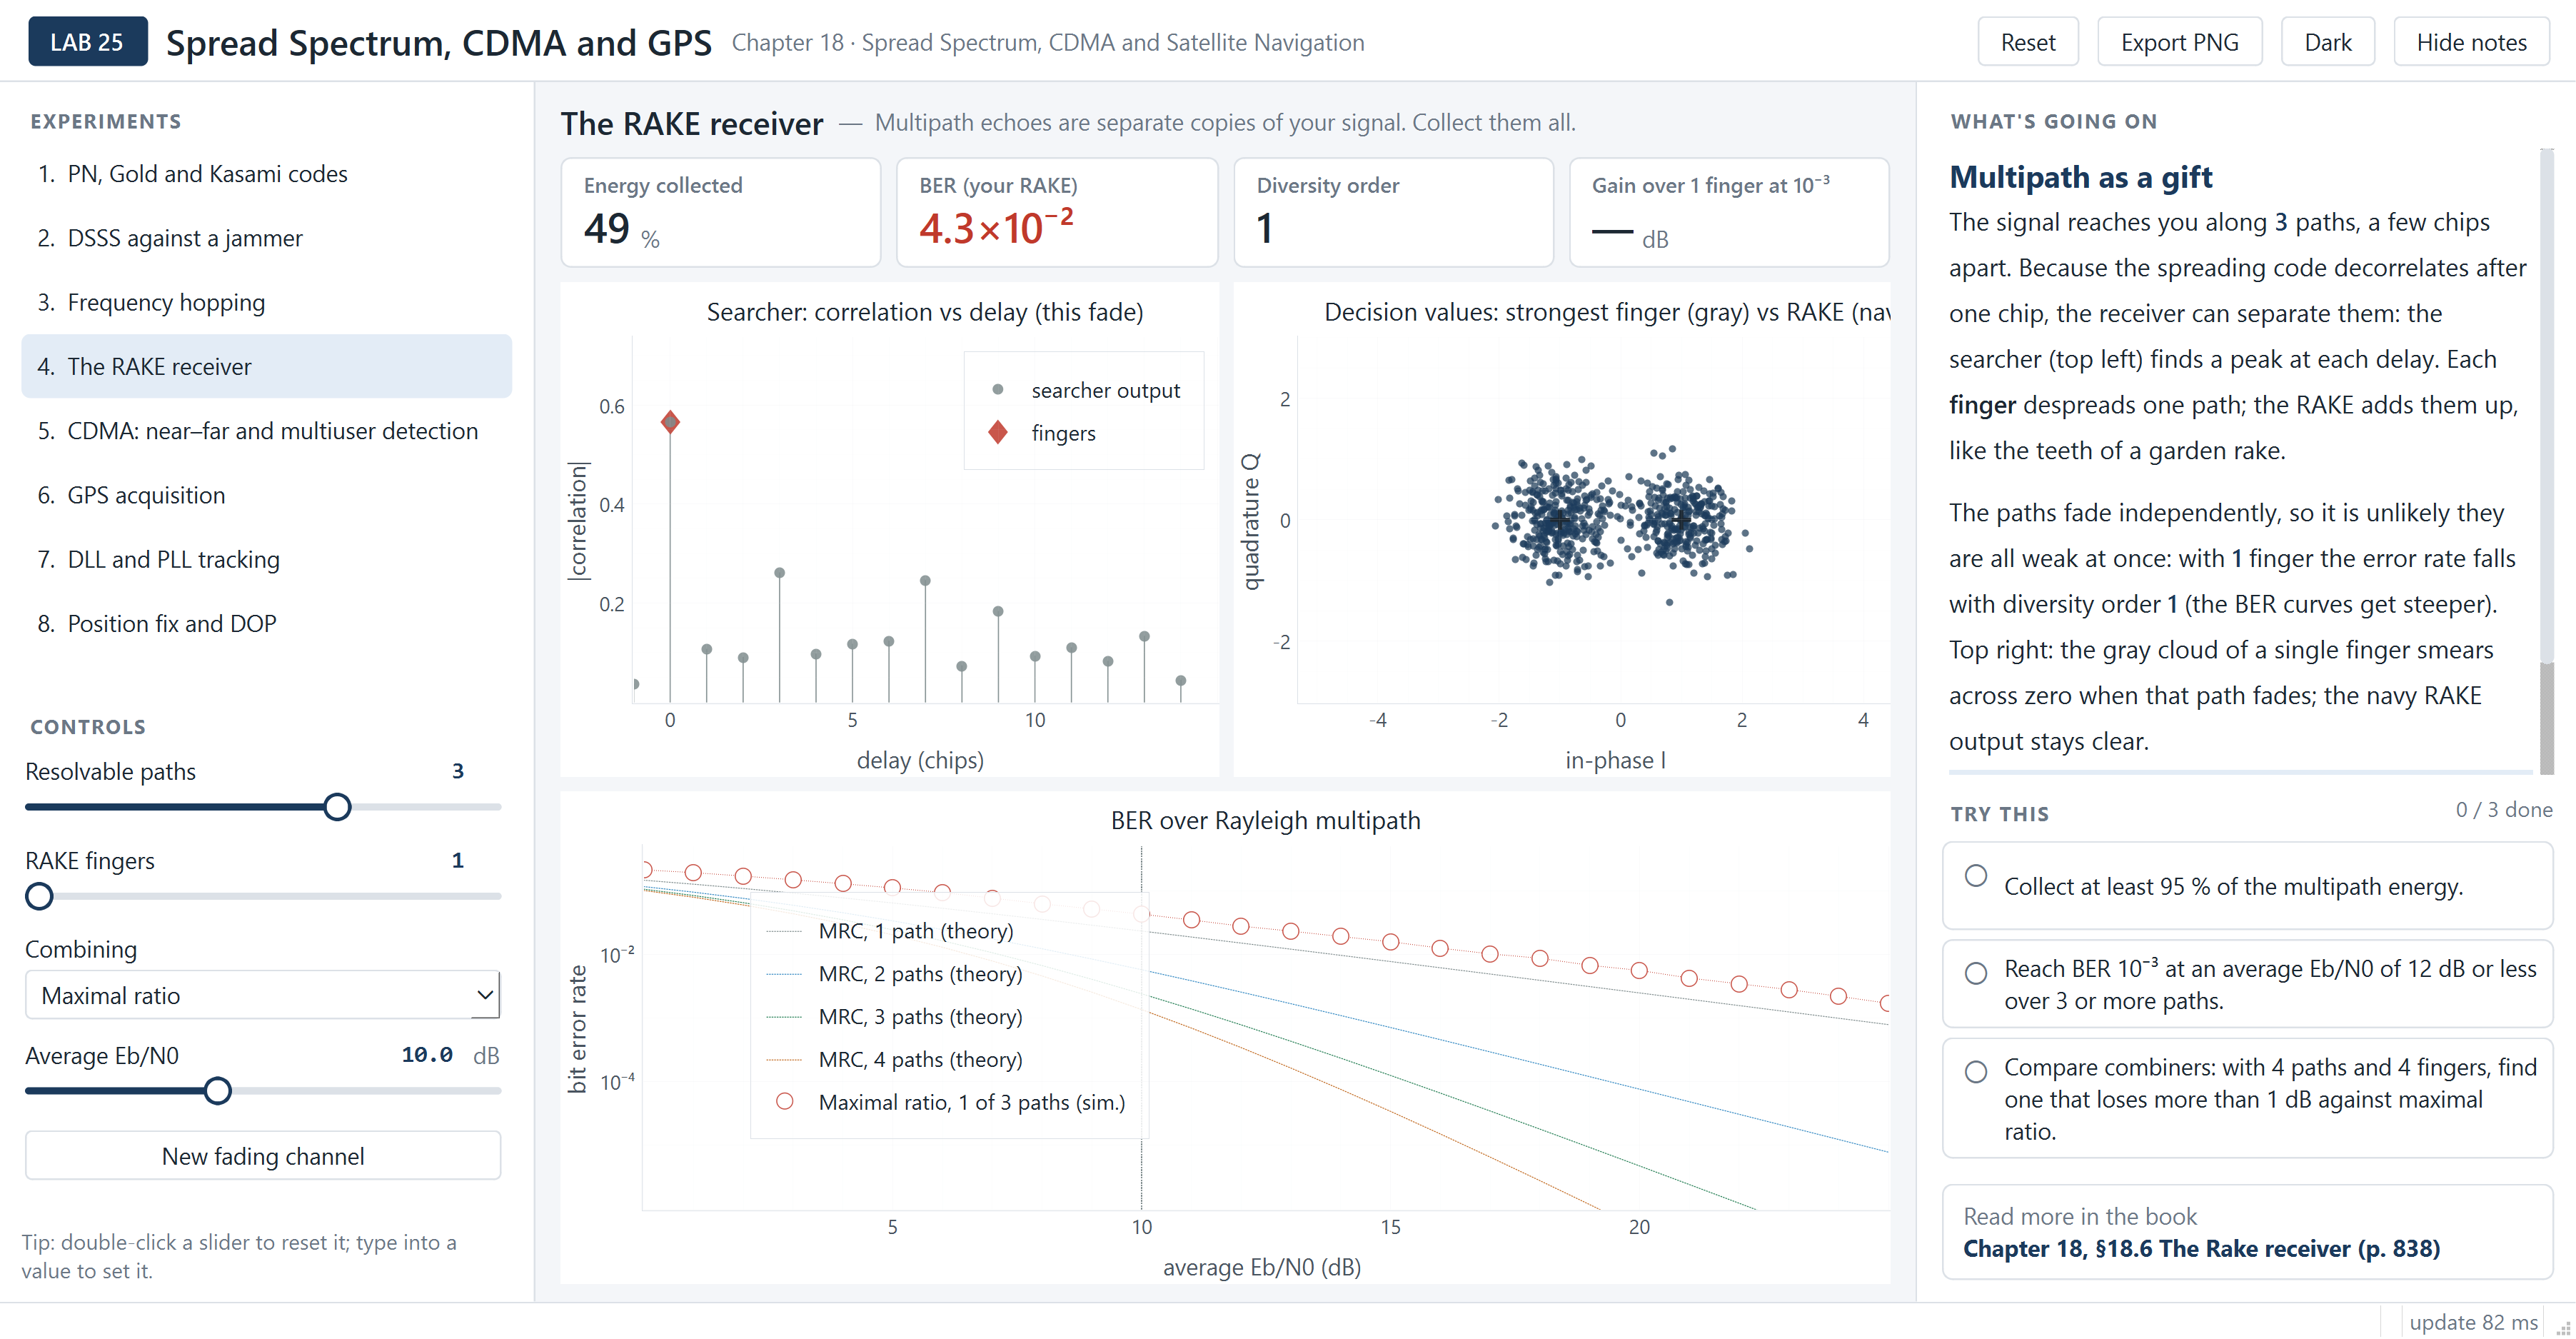
\includegraphics[width=0.72\linewidth]{figs/ch18_lab_e4}
\caption{Lab~25's \emph{The RAKE receiver} with three resolvable paths and a single finger: the
searcher sees three peaks, but one finger collects only about half the energy and the error rate
sits on the single-path Rayleigh line. Add fingers and watch the BER curve steepen.}
\label{fig:ch18_lab_e4}\end{figure}

\begin{labbox}[Spread spectrum, CDMA and a GPS receiver from scratch]
The lab for this chapter is the interactive app
\begin{itemize}
\item \lab{moderncomms-labs/labs/lab25\_spread\_spectrum\_gps.py} (run it with
\lab{python labs/lab25\_spread\_spectrum\_gps.py}).
\end{itemize}
It has eight experiments, each tied to a section of this chapter:
\begin{itemize}
\item \textbf{PN, Gold and Kasami codes} (Section~\ref{sec:ch18:pn}): build LFSR, Gold, Kasami and
GPS C/A codes and check their auto- and cross-correlations against the theory bounds.
\item \textbf{DSSS against a jammer} (Section~\ref{sec:ch18:jamming}): spread and despread BPSK
against a tone or narrowband-noise jammer and measure the jamming margin
(Figures~\ref{fig:ch18_jammer_spectra} and~\ref{fig:ch18_dsss_ber}).
\item \textbf{Frequency hopping} (Section~\ref{sec:ch18:fhss}, Figure~\ref{fig:ch18_lab_e3}): hop
around a Wi-Fi network with and without adaptive hopping, and play against a partial-band jammer
with diversity.
\item \textbf{The RAKE receiver} (Section~\ref{sec:ch18:rake}, Figure~\ref{fig:ch18_lab_e4}): fingers, maximal-ratio, equal-gain
and selection combining on a fading multipath channel.
\item \textbf{CDMA: near--far and multiuser detection} (Section~\ref{sec:ch18:mud}): a small CDMA
uplink with the near--far problem, power control, and the decorrelator, MMSE and SIC detectors.
\item \textbf{GPS acquisition} (Section~\ref{sec:ch18:acq}): the delay--Doppler search of
Figure~\ref{fig:ch18_acquisition} on a synthetic multi-satellite L1 signal buried in noise.
\item \textbf{DLL and PLL tracking} (Section~\ref{sec:ch18:tracking}): a live tracking channel with
an FLL-assisted Costas PLL and an early--late DLL that reads the navigation bits.
\item \textbf{Position fix and DOP} (Section~\ref{sec:ch18:errors}): solve for position and clock
from pseudoranges by Gauss--Newton and watch geometry stretch the error cloud.
\end{itemize}
All the tools are in \lab{moderncomms-labs/commlib/spread.py}, and \lab{book/figscripts/ch18\_figs.py}
generates every data figure in the chapter.
\end{labbox}

\problems
\begin{enumerate}[label=\thechapter.\arabic*]
\item A DSSS system has a chip rate of 10\,Mchip/s and carries 10\,kb/s of data. What is its
processing gain? If the required $E_b/J_0$ is 8\,dB and implementation losses are 2\,dB, what is
the jamming margin? How does a rate-1/2 code with 5\,dB of coding gain change it (assume the
chip rate is fixed)?
\item Find the period, the number of ones and the run-length distribution of the sequence
generated by $x^4+x+1$ from the state 0001. Verify the two-valued autocorrelation. Repeat for
$x^4+x^3+x^2+x+1$ and explain what goes wrong.
\item Prove the shift-and-add property of m-sequences from the linear recurrence, and use it to
derive~\eqref{eq:ch18:mseqacf}. Then show that the PSD of the periodic $\pm1$ chip waveform is
given by~\eqref{eq:ch18:pnpsd}.
\item Using the Welch bound~\eqref{eq:ch18:welch}, compare the maximum correlation of the GPS Gold
family ($N=1023$, $K=1025$) and of the small Kasami set ($N=1023$, $K=32$) with the bound. How
many decibels below the peak is the worst cross-correlation in each case?
\item Construct the OVSF codes of spreading factor 8. A user at SF\,4 is assigned $C_{4,1}$. Which
SF\,8 codes are blocked? Compute the cross-correlation of $C_{8,2}$ and $C_{8,3}$ with a one-chip
offset.
\item Derive the worst-case pulsed-jamming result for DS-BPSK. Show that the bit error
probability $P_b(\rho)=\rho\,\Q\big(\sqrt{2\rho E_b/J_0}\big)$ is maximised at
$\rho\approx0.71/(E_b/J_0)$, which gives $P_b\approx0.083/(E_b/J_0)$.
\item Using~\eqref{eq:ch18:capacity}, estimate the number of users per sector of a WCDMA carrier
carrying 12.2\,kb/s voice at a required $E_b/I_0$ of 5\,dB, with $\nu=0.5$, $f=0.65$ and three
sectors with $G_s=2.5$. Then include the loading: what is the noise rise at 70\% of this pole
capacity, and how much does it shrink the cell radius with a path-loss exponent of 3.5?
\item Two users of a synchronous CDMA system have codes with normalised cross-correlation
$\rho=0.25$ and amplitudes $A_1=1$, $A_2=10$. Find the BER of user 1 at $E_b/N_0=10$\,dB with
(a) the conventional detector (conditioning on user 2's bit), and (b) the decorrelator. Explain
why the decorrelator's result does not depend on $A_2$.
\item Show that maximal-ratio combining maximises the output SNR of a Rake receiver (use
Cauchy--Schwarz) and derive~\eqref{eq:ch18:mrc}. For two paths of mean SNR 10\,dB each, compute
the probability that the combined SNR falls below 3\,dB, and compare with a single path of mean
SNR 13\,dB.
\item A LoRa link uses SF\,10, 125\,kHz and a rate-4/5 code. Find the symbol time, the bit rate
and the time on air of a 20-byte payload (ignore the header and preamble). How many such
packets per hour can one device send under a 1\% duty-cycle limit?
\item Linearise the pseudorange equations and derive~\eqref{eq:ch18:linear}. For four satellites
at azimuths 0$^\circ$, 120$^\circ$ and 240$^\circ$ at 30$^\circ$ elevation plus one at the
zenith, compute HDOP, VDOP and TDOP (work in local east--north--up coordinates).
\item Compute the general- and special-relativistic rate offsets of a Galileo satellite
(semi-major axis 29\,600\,km) and of a geostationary satellite. Express each in microseconds per
day and in the equivalent range error per day.
\item A receiver integrates coherently for $T$ and the residual frequency error is uniform within
$\pm\Delta f/2$. Find the average loss $\E[\sinc^2(fT)]$ for bin widths $\Delta f=1/(2T)$, $2/(3T)$
and $1/T$. Which bin width minimises the total search time for a given detection performance?
\item \emph{(Simulation)} Generate the C/A codes for PRN 1--32 with
\lab{spread.gps\_ca\_code} and verify the first ten chips against the octal values in
IS-GPS-200. Compute all periodic auto- and cross-correlations and confirm that they take only the
values $-1$, $-65$ and $63$ off the peak. Then compute the cross-correlation when one code has a
Doppler offset of 1, 3 and 5\,kHz over 1\,ms, and explain the result.
\item \emph{(Simulation)} Synthesise one second of a four-satellite L1 C/A signal using the
function \lab{spread.gps\_baseband} at $C/N_0$ between 35 and 48\,dB-Hz. Acquire all four satellites,
track them, extract the code phases at a common instant and, given the satellite positions,
solve for the receiver position and clock offset. Repeat with a CW jammer at 1575.42\,MHz plus
3\,kHz and find the J/S at which each satellite is lost.
\end{enumerate}

\furtherreading
\begin{itemize}
\item E.~D.~Kaplan and C.~J.~Hegarty (eds.), \emph{Understanding GPS/GNSS: Principles and
Applications}, 3rd ed., Artech House, 2017. The standard engineering reference on GNSS signals,
receivers, errors and augmentation.
\item P.~Misra and P.~Enge, \emph{Global Positioning System: Signals, Measurements, and
Performance}, 2nd ed., Ganga-Jamuna Press, 2006. The clearest introduction to the measurement
models, DOP, differential and carrier-phase positioning.
\item K.~Borre, D.~M.~Akos, N.~Bertelsen, P.~Rinder and S.~H.~Jensen, \emph{A Software-Defined GPS
and Galileo Receiver: A Single-Frequency Approach}, Birkh\"auser, 2007. A complete MATLAB
software receiver with acquisition, tracking and navigation; the model for the lab.
\item J.~W.~Betz, \emph{Engineering Satellite-Based Navigation and Timing: Global Navigation
Satellite Systems, Signals, and Receivers}, Wiley-IEEE Press, 2016. Signal design (BOC, MBOC),
correlation and receiver processing in depth, by the designer of BOC.
\item B.~W.~Parkinson and J.~J.~Spilker Jr.\ (eds.), \emph{Global Positioning System: Theory and
Applications}, 2 vols., AIAA, 1996. The founders' own account of GPS design.
\item IS-GPS-200 (\emph{NAVSTAR GPS Space Segment/Navigation User Interfaces}), IS-GPS-705 (L5)
and IS-GPS-800 (L1C), current revisions. The interface specifications: code tables, message
formats, received power levels and the user algorithms.
\item A.~J.~Viterbi, \emph{CDMA: Principles of Spread Spectrum Communication}, Addison-Wesley,
1995. CDMA theory by one of its principal architects: capacity, power control, soft handoff.
\item K.~S.~Gilhousen, I.~M.~Jacobs, R.~Padovani, A.~J.~Viterbi, L.~A.~Weaver and C.~E.~Wheatley,
``On the capacity of a cellular CDMA system,'' \emph{IEEE Transactions on Vehicular Technology},
vol.~40, no.~2, 1991. The paper that made the case for cellular CDMA.
\item M.~K.~Simon, J.~K.~Omura, R.~A.~Scholtz and B.~K.~Levitt, \emph{Spread Spectrum
Communications Handbook}, revised ed., McGraw-Hill, 1994. Anti-jam performance, pulsed and
partial-band jamming, and synchronisation, from the military tradition.
\item R.~A.~Scholtz, ``The origins of spread-spectrum communications,'' \emph{IEEE Transactions on
Communications}, vol.~30, no.~5, 1982. The history, from the participants.
\item D.~V.~Sarwate and M.~B.~Pursley, ``Crosscorrelation properties of pseudorandom and related
sequences,'' \emph{Proceedings of the IEEE}, vol.~68, no.~5, 1980. The classic survey of
m-sequences, Gold and Kasami codes.
\item S.~Verd\'u, \emph{Multiuser Detection}, Cambridge University Press, 1998. The definitive
treatment of optimum and linear multiuser detectors.
\end{itemize}
